\documentclass[twoside]{book}

% Packages required by doxygen
\usepackage{calc}
\usepackage{doxygen}
\usepackage{graphicx}
\usepackage[utf8]{inputenc}
\usepackage{makeidx}
\usepackage{multicol}
\usepackage{multirow}
\usepackage{textcomp}
\usepackage[table]{xcolor}

% Font selection
\usepackage[T1]{fontenc}
\usepackage{mathptmx}
\usepackage[scaled=.90]{helvet}
\usepackage{courier}
\usepackage{amssymb}
\usepackage{sectsty}
\renewcommand{\familydefault}{\sfdefault}
\allsectionsfont{%
  \fontseries{bc}\selectfont%
  \color{darkgray}%
}
\renewcommand{\DoxyLabelFont}{%
  \fontseries{bc}\selectfont%
  \color{darkgray}%
}

% Page & text layout
\usepackage{geometry}
\geometry{%
  a4paper,%
  top=2.5cm,%
  bottom=2.5cm,%
  left=2.5cm,%
  right=2.5cm%
}
\tolerance=750
\hfuzz=15pt
\hbadness=750
\setlength{\emergencystretch}{15pt}
\setlength{\parindent}{0cm}
\setlength{\parskip}{0.2cm}
\makeatletter
\renewcommand{\paragraph}{%
  \@startsection{paragraph}{4}{0ex}{-1.0ex}{1.0ex}{%
    \normalfont\normalsize\bfseries\SS@parafont%
  }%
}
\renewcommand{\subparagraph}{%
  \@startsection{subparagraph}{5}{0ex}{-1.0ex}{1.0ex}{%
    \normalfont\normalsize\bfseries\SS@subparafont%
  }%
}
\makeatother

% Headers & footers
\usepackage{fancyhdr}
\pagestyle{fancyplain}
\fancyhead[LE]{\fancyplain{}{\bfseries\thepage}}
\fancyhead[CE]{\fancyplain{}{}}
\fancyhead[RE]{\fancyplain{}{\bfseries\leftmark}}
\fancyhead[LO]{\fancyplain{}{\bfseries\rightmark}}
\fancyhead[CO]{\fancyplain{}{}}
\fancyhead[RO]{\fancyplain{}{\bfseries\thepage}}
\fancyfoot[LE]{\fancyplain{}{}}
\fancyfoot[CE]{\fancyplain{}{}}
\fancyfoot[RE]{\fancyplain{}{\bfseries\scriptsize Generated on Sat Jul 9 2016 16\-:24\-:44 for V\-S\-S-\/\-Vision by Doxygen }}
\fancyfoot[LO]{\fancyplain{}{\bfseries\scriptsize Generated on Sat Jul 9 2016 16\-:24\-:44 for V\-S\-S-\/\-Vision by Doxygen }}
\fancyfoot[CO]{\fancyplain{}{}}
\fancyfoot[RO]{\fancyplain{}{}}
\renewcommand{\footrulewidth}{0.4pt}
\renewcommand{\chaptermark}[1]{%
  \markboth{#1}{}%
}
\renewcommand{\sectionmark}[1]{%
  \markright{\thesection\ #1}%
}

% Indices & bibliography
\usepackage{natbib}
\usepackage[titles]{tocloft}
\setcounter{tocdepth}{3}
\setcounter{secnumdepth}{5}
\makeindex

% Hyperlinks (required, but should be loaded last)
\usepackage{ifpdf}
\ifpdf
  \usepackage[pdftex,pagebackref=true]{hyperref}
\else
  \usepackage[ps2pdf,pagebackref=true]{hyperref}
\fi
\hypersetup{%
  colorlinks=true,%
  linkcolor=blue,%
  citecolor=blue,%
  unicode%
}

% Custom commands
\newcommand{\clearemptydoublepage}{%
  \newpage{\pagestyle{empty}\cleardoublepage}%
}


%===== C O N T E N T S =====

\begin{document}

% Titlepage & ToC
\hypersetup{pageanchor=false}
\pagenumbering{roman}
\begin{titlepage}
\vspace*{7cm}
\begin{center}%
{\Large V\-S\-S-\/\-Vision }\\
\vspace*{1cm}
{\large Generated by Doxygen 1.8.6}\\
\vspace*{0.5cm}
{\small Sat Jul 9 2016 16:24:44}\\
\end{center}
\end{titlepage}
\clearemptydoublepage
\tableofcontents
\clearemptydoublepage
\pagenumbering{arabic}
\hypersetup{pageanchor=true}

%--- Begin generated contents ---
\chapter{Namespace Index}
\section{Namespace List}
Here is a list of all documented namespaces with brief descriptions\-:\begin{DoxyCompactList}
\item\contentsline{section}{\hyperlink{namespacecommon}{common} \\*This namespace is responsible to implement all global functions and custom datatypes used in the software, like\-: E\-N\-U\-M\-S, \hyperlink{structcommon_1_1btVector3}{bt\-Vector3}, \hyperlink{structcommon_1_1Pixel}{Pixel}, \hyperlink{structcommon_1_1TableColor}{Table\-Color}, \hyperlink{structcommon_1_1VisionColor}{Vision\-Color}, \hyperlink{structcommon_1_1ExecConfiguration}{Exec\-Configuration}, \hyperlink{structcommon_1_1Calibration}{Calibration}, \hyperlink{structcommon_1_1Robot}{Robot} and \hyperlink{structcommon_1_1State}{State} }{\pageref{namespacecommon}}{}
\end{DoxyCompactList}

\chapter{Hierarchical Index}
\section{Class Hierarchy}
This inheritance list is sorted roughly, but not completely, alphabetically\+:\begin{DoxyCompactList}
\item \contentsline{section}{common\+:\+:bt\+Vector3}{\pageref{structcommon_1_1btVector3}}{}
\item \contentsline{section}{common\+:\+:Calibration}{\pageref{structcommon_1_1Calibration}}{}
\item \contentsline{section}{common\+:\+:Exec\+Configuration}{\pageref{structcommon_1_1ExecConfiguration}}{}
\item \contentsline{section}{Interface}{\pageref{classInterface}}{}
\item Message\begin{DoxyCompactList}
\item \contentsline{section}{vss\+\_\+command\+:\+:Global\+\_\+\+Commands}{\pageref{classvss__command_1_1Global__Commands}}{}
\item \contentsline{section}{vss\+\_\+command\+:\+:Robot\+\_\+\+Command}{\pageref{classvss__command_1_1Robot__Command}}{}
\item \contentsline{section}{vss\+\_\+state\+:\+:Global\+\_\+\+State}{\pageref{classvss__state_1_1Global__State}}{}
\item \contentsline{section}{vss\+\_\+state\+:\+:Pose}{\pageref{classvss__state_1_1Pose}}{}
\item \contentsline{section}{vss\+\_\+state\+:\+:R\+GB}{\pageref{classvss__state_1_1RGB}}{}
\item \contentsline{section}{vss\+\_\+state\+:\+:Robot\+\_\+\+State}{\pageref{classvss__state_1_1Robot__State}}{}
\end{DoxyCompactList}
\item \contentsline{section}{common\+:\+:Pixel}{\pageref{structcommon_1_1Pixel}}{}
\item Q\+Label\begin{DoxyCompactList}
\item \contentsline{section}{Q\+Custom\+Label}{\pageref{classQCustomLabel}}{}
\end{DoxyCompactList}
\item Q\+Main\+Window\begin{DoxyCompactList}
\item \contentsline{section}{Main\+Window}{\pageref{classMainWindow}}{}
\end{DoxyCompactList}
\item Q\+Thread\begin{DoxyCompactList}
\item \contentsline{section}{calibration}{\pageref{classcalibration}}{}
\item \contentsline{section}{vision}{\pageref{classvision}}{}
\end{DoxyCompactList}
\item \contentsline{section}{common\+:\+:Robot}{\pageref{structcommon_1_1Robot}}{}
\item \contentsline{section}{S\+Q\+Lite}{\pageref{classSQLite}}{}
\item \contentsline{section}{common\+:\+:State}{\pageref{structcommon_1_1State}}{}
\item \contentsline{section}{vss\+\_\+command\+:\+:Static\+Descriptor\+Initializer\+\_\+command\+\_\+2eproto}{\pageref{structvss__command_1_1StaticDescriptorInitializer__command__2eproto}}{}
\item \contentsline{section}{vss\+\_\+state\+:\+:Static\+Descriptor\+Initializer\+\_\+state\+\_\+2eproto}{\pageref{structvss__state_1_1StaticDescriptorInitializer__state__2eproto}}{}
\item \contentsline{section}{common\+:\+:Table\+Color}{\pageref{structcommon_1_1TableColor}}{}
\item \contentsline{section}{common\+:\+:Vision\+Color}{\pageref{structcommon_1_1VisionColor}}{}
\end{DoxyCompactList}

\chapter{Class Index}
\section{Class List}
Here are the classes, structs, unions and interfaces with brief descriptions\+:\begin{DoxyCompactList}
\item\contentsline{section}{\hyperlink{structcommon_1_1btVector3}{common\+::bt\+Vector3} \\*This struct represents a Vector in R$^\wedge$3 }{\pageref{structcommon_1_1btVector3}}{}
\item\contentsline{section}{\hyperlink{classcalibration}{calibration} \\*This class is responsible for calibrate all \hyperlink{structcommon_1_1VisionColor}{common\+::\+Vision\+Color}, cut points and rotation }{\pageref{classcalibration}}{}
\item\contentsline{section}{\hyperlink{structcommon_1_1Calibration}{common\+::\+Calibration} \\*This struct represents a calibration of colors }{\pageref{structcommon_1_1Calibration}}{}
\item\contentsline{section}{\hyperlink{structcommon_1_1ExecConfiguration}{common\+::\+Exec\+Configuration} \\*This struct represents a configuration of colors of objects in workspace }{\pageref{structcommon_1_1ExecConfiguration}}{}
\item\contentsline{section}{\hyperlink{classvss__command_1_1Global__Commands}{vss\+\_\+command\+::\+Global\+\_\+\+Commands} }{\pageref{classvss__command_1_1Global__Commands}}{}
\item\contentsline{section}{\hyperlink{classvss__state_1_1Global__State}{vss\+\_\+state\+::\+Global\+\_\+\+State} }{\pageref{classvss__state_1_1Global__State}}{}
\item\contentsline{section}{\hyperlink{classInterface}{Interface} \\*This class is responsible for handle the communicatio between V\+S\+S-\/\+Vision, V\+S\+S-\/\+Simulator, V\+S\+S-\/\+Viewer and V\+S\+S-\/\+Sample\+Strategy }{\pageref{classInterface}}{}
\item\contentsline{section}{\hyperlink{classMainWindow}{Main\+Window} \\*This class is the main window of the software }{\pageref{classMainWindow}}{}
\item\contentsline{section}{\hyperlink{structcommon_1_1Pixel}{common\+::\+Pixel} \\*This struct represents a \hyperlink{structcommon_1_1Pixel}{Pixel}, can be\+: R\+GB and H\+SV. It\textquotesingle{}s used float because is possible to represent color in systems, like\+: 0 to 1, and 0 to 255 }{\pageref{structcommon_1_1Pixel}}{}
\item\contentsline{section}{\hyperlink{classvss__state_1_1Pose}{vss\+\_\+state\+::\+Pose} }{\pageref{classvss__state_1_1Pose}}{}
\item\contentsline{section}{\hyperlink{classQCustomLabel}{Q\+Custom\+Label} \\*This class is a modification of Q\+Label, \hyperlink{classQCustomLabel}{Q\+Custom\+Label} handle events like\+: mouse click, mouse move, scrool wheel move and etc }{\pageref{classQCustomLabel}}{}
\item\contentsline{section}{\hyperlink{classvss__state_1_1RGB}{vss\+\_\+state\+::\+R\+GB} }{\pageref{classvss__state_1_1RGB}}{}
\item\contentsline{section}{\hyperlink{structcommon_1_1Robot}{common\+::\+Robot} \\*This strcut represets the pose that one robot can handle. Pos and Vel }{\pageref{structcommon_1_1Robot}}{}
\item\contentsline{section}{\hyperlink{classvss__command_1_1Robot__Command}{vss\+\_\+command\+::\+Robot\+\_\+\+Command} }{\pageref{classvss__command_1_1Robot__Command}}{}
\item\contentsline{section}{\hyperlink{classvss__state_1_1Robot__State}{vss\+\_\+state\+::\+Robot\+\_\+\+State} }{\pageref{classvss__state_1_1Robot__State}}{}
\item\contentsline{section}{\hyperlink{classSQLite}{S\+Q\+Lite} \\*This class is responsible for create, read, update and delete \hyperlink{structcommon_1_1Calibration}{common\+::\+Calibration} \textquotesingle{}s and \hyperlink{structcommon_1_1ExecConfiguration}{common\+::\+Exec\+Configuration} \textquotesingle{}s }{\pageref{classSQLite}}{}
\item\contentsline{section}{\hyperlink{structcommon_1_1State}{common\+::\+State} \\*This struct represents the state that the workspace can handle }{\pageref{structcommon_1_1State}}{}
\item\contentsline{section}{\hyperlink{structvss__command_1_1StaticDescriptorInitializer__command__2eproto}{vss\+\_\+command\+::\+Static\+Descriptor\+Initializer\+\_\+command\+\_\+2eproto} }{\pageref{structvss__command_1_1StaticDescriptorInitializer__command__2eproto}}{}
\item\contentsline{section}{\hyperlink{structvss__state_1_1StaticDescriptorInitializer__state__2eproto}{vss\+\_\+state\+::\+Static\+Descriptor\+Initializer\+\_\+state\+\_\+2eproto} }{\pageref{structvss__state_1_1StaticDescriptorInitializer__state__2eproto}}{}
\item\contentsline{section}{\hyperlink{structcommon_1_1TableColor}{common\+::\+Table\+Color} \\*This struct represents all colors in R\+GB that can be used }{\pageref{structcommon_1_1TableColor}}{}
\item\contentsline{section}{\hyperlink{classvision}{vision} \\*This class is responsible for track all objects in field }{\pageref{classvision}}{}
\item\contentsline{section}{\hyperlink{structcommon_1_1VisionColor}{common\+::\+Vision\+Color} \\*This struct represents a Color that can be calibrated\+: made by 2 Pixels that represents a range of color, Bottom \hyperlink{structcommon_1_1Pixel}{Pixel} Limit and Top \hyperlink{structcommon_1_1Pixel}{Pixel} Limit }{\pageref{structcommon_1_1VisionColor}}{}
\end{DoxyCompactList}

\chapter{Namespace Documentation}
\hypertarget{namespacecommon}{}\section{common Namespace Reference}
\label{namespacecommon}\index{common@{common}}


This namespace is responsible to implement all global functions and custom datatypes used in the software, like\+: E\+N\+U\+MS, \hyperlink{structcommon_1_1btVector3}{bt\+Vector3}, \hyperlink{structcommon_1_1Pixel}{Pixel}, \hyperlink{structcommon_1_1TableColor}{Table\+Color}, \hyperlink{structcommon_1_1VisionColor}{Vision\+Color}, \hyperlink{structcommon_1_1ExecConfiguration}{Exec\+Configuration}, \hyperlink{structcommon_1_1Calibration}{Calibration}, \hyperlink{structcommon_1_1Robot}{Robot} and \hyperlink{structcommon_1_1State}{State}.  


\subsection*{Classes}
\begin{DoxyCompactItemize}
\item 
struct \hyperlink{structcommon_1_1btVector3}{bt\+Vector3}
\begin{DoxyCompactList}\small\item\em This struct represents a Vector in R$^\wedge$3. \end{DoxyCompactList}\item 
struct \hyperlink{structcommon_1_1Calibration}{Calibration}
\begin{DoxyCompactList}\small\item\em This struct represents a calibration of colors. \end{DoxyCompactList}\item 
struct \hyperlink{structcommon_1_1ExecConfiguration}{Exec\+Configuration}
\begin{DoxyCompactList}\small\item\em This struct represents a configuration of colors of objects in workspace. \end{DoxyCompactList}\item 
struct \hyperlink{structcommon_1_1Pixel}{Pixel}
\begin{DoxyCompactList}\small\item\em This struct represents a \hyperlink{structcommon_1_1Pixel}{Pixel}, can be\+: R\+GB and H\+SV. It\textquotesingle{}s used float because is possible to represent color in systems, like\+: 0 to 1, and 0 to 255. \end{DoxyCompactList}\item 
struct \hyperlink{structcommon_1_1Robot}{Robot}
\begin{DoxyCompactList}\small\item\em This strcut represets the pose that one robot can handle. Pos and Vel. \end{DoxyCompactList}\item 
struct \hyperlink{structcommon_1_1State}{State}
\begin{DoxyCompactList}\small\item\em This struct represents the state that the workspace can handle. \end{DoxyCompactList}\item 
struct \hyperlink{structcommon_1_1TableColor}{Table\+Color}
\begin{DoxyCompactList}\small\item\em This struct represents all colors in R\+GB that can be used. \end{DoxyCompactList}\item 
struct \hyperlink{structcommon_1_1VisionColor}{Vision\+Color}
\begin{DoxyCompactList}\small\item\em This struct represents a Color that can be calibrated\+: made by 2 Pixels that represents a range of color, Bottom \hyperlink{structcommon_1_1Pixel}{Pixel} Limit and Top \hyperlink{structcommon_1_1Pixel}{Pixel} Limit. \end{DoxyCompactList}\end{DoxyCompactItemize}
\subsection*{Enumerations}
\begin{DoxyCompactItemize}
\item 
enum \{ {\bfseries r} = 0, 
{\bfseries g} = 1, 
{\bfseries b} = 2
 \}\hypertarget{namespacecommon_a491fb143df4d6e143a19de8d5863ef28}{}\label{namespacecommon_a491fb143df4d6e143a19de8d5863ef28}
\begin{DoxyCompactList}\small\item\em This enum implements a abstraction of a R\+GB array. \end{DoxyCompactList}
\item 
enum \{ \\*
{\bfseries rmin} = 0, 
{\bfseries gmin} = 1, 
{\bfseries bmin} = 2, 
{\bfseries rmax} = 3, 
\\*
{\bfseries gmax} = 4, 
{\bfseries bmax} = 5
 \}\hypertarget{namespacecommon_a497fe38f750672b3984a9099aa7b7eed}{}\label{namespacecommon_a497fe38f750672b3984a9099aa7b7eed}
\begin{DoxyCompactList}\small\item\em This enum implements a abstraction of a range of R\+GB array. \end{DoxyCompactList}
\item 
enum \{ {\bfseries h} = 0, 
{\bfseries s} = 1, 
{\bfseries v} = 2
 \}\hypertarget{namespacecommon_ad19e2da0c005a20bb6e218b5393d0994}{}\label{namespacecommon_ad19e2da0c005a20bb6e218b5393d0994}
\begin{DoxyCompactList}\small\item\em This enum implements a abstraction of a H\+SV array. \end{DoxyCompactList}
\item 
enum \{ \\*
{\bfseries hmin} = 0, 
{\bfseries smin} = 1, 
{\bfseries vmin} = 2, 
{\bfseries hmax} = 3, 
\\*
{\bfseries smax} = 4, 
{\bfseries vmax} = 5
 \}\hypertarget{namespacecommon_aca4dbe5edbfb61860448876cc31ea0d6}{}\label{namespacecommon_aca4dbe5edbfb61860448876cc31ea0d6}
\begin{DoxyCompactList}\small\item\em This enum implements a abstraction of a range of H\+SV array. \end{DoxyCompactList}
\item 
enum \{ {\bfseries O\+U\+R\+\_\+\+T\+E\+AM} = 0, 
{\bfseries A\+D\+V\+E\+R\+S\+A\+R\+Y\+\_\+\+T\+E\+AM} = 1
 \}\hypertarget{namespacecommon_a9282a476d6b9d03ef99617079881fa46}{}\label{namespacecommon_a9282a476d6b9d03ef99617079881fa46}
\begin{DoxyCompactList}\small\item\em This enum implements a abstraction of teams. \end{DoxyCompactList}
\item 
enum \{ \\*
{\bfseries O\+R\+A\+N\+GE} = 0, 
{\bfseries B\+L\+UE} = 1, 
{\bfseries Y\+E\+L\+L\+OW} = 2, 
{\bfseries R\+ED} = 3, 
\\*
{\bfseries P\+I\+NK} = 4, 
{\bfseries P\+U\+R\+P\+LE} = 5, 
{\bfseries G\+R\+E\+EN} = 6, 
{\bfseries B\+R\+O\+WN} = 7, 
\\*
{\bfseries R\+O\+T\+A\+T\+I\+ON} = 8, 
{\bfseries C\+UT} = 9
 \}\hypertarget{namespacecommon_a8993f678d3732043cfd91d1ecff7aee9}{}\label{namespacecommon_a8993f678d3732043cfd91d1ecff7aee9}
\begin{DoxyCompactList}\small\item\em ! This enum represents all data that can be calibrated. \end{DoxyCompactList}
\item 
enum \{ {\bfseries S\+Q\+U\+A\+R\+ES} = 0, 
{\bfseries R\+E\+C\+T\+A\+N\+G\+L\+ES} = 1, 
{\bfseries C\+I\+R\+C\+L\+ES} = 2
 \}\hypertarget{namespacecommon_a8714be2ce7f79e894ea222f8b6c6192d}{}\label{namespacecommon_a8714be2ce7f79e894ea222f8b6c6192d}
\begin{DoxyCompactList}\small\item\em This enum represents all types of blob that can be used. \end{DoxyCompactList}
\item 
enum \{ {\bfseries U\+N\+K\+N\+O\+WN} = -\/1
 \}\hypertarget{namespacecommon_a778707b5ddd121964dfde87ca9412cdd}{}\label{namespacecommon_a778707b5ddd121964dfde87ca9412cdd}
\begin{DoxyCompactList}\small\item\em This enum represents all unknown things. \end{DoxyCompactList}
\item 
enum \{ {\bfseries C\+A\+M\+E\+RA} = 0, 
{\bfseries I\+M\+A\+GE} = 1, 
{\bfseries V\+I\+D\+EO} = 2
 \}\hypertarget{namespacecommon_aa3ff310c0126c187a017a24df9b33bb0}{}\label{namespacecommon_aa3ff310c0126c187a017a24df9b33bb0}
\begin{DoxyCompactList}\small\item\em This enum represents all types of input datas. \end{DoxyCompactList}
\item 
enum \{ \\*
{\bfseries B\+A\+LL} = 0, 
{\bfseries T\+E\+A\+M1\+\_\+\+R\+O\+B\+O\+T1} = 1, 
{\bfseries T\+E\+A\+M1\+\_\+\+R\+O\+B\+O\+T2} = 2, 
{\bfseries T\+E\+A\+M1\+\_\+\+R\+O\+B\+O\+T3} = 3, 
\\*
{\bfseries T\+E\+A\+M2\+\_\+\+R\+O\+B\+O\+T1} = 4, 
{\bfseries T\+E\+A\+M2\+\_\+\+R\+O\+B\+O\+T2} = 5, 
{\bfseries T\+E\+A\+M2\+\_\+\+R\+O\+B\+O\+T3} = 6
 \}\hypertarget{namespacecommon_a621a02b7b7574c1037f6e656ad8646e5}{}\label{namespacecommon_a621a02b7b7574c1037f6e656ad8646e5}
\begin{DoxyCompactList}\small\item\em This enum represents all objects in a State. \end{DoxyCompactList}
\end{DoxyCompactItemize}
\subsection*{Functions}
\begin{DoxyCompactItemize}
\item 
void \hyperlink{namespacecommon_aa388eb4aec4a6c1fc25e4af17bcd35b6}{clear\+SS} (stringstream \&ss)\hypertarget{namespacecommon_aa388eb4aec4a6c1fc25e4af17bcd35b6}{}\label{namespacecommon_aa388eb4aec4a6c1fc25e4af17bcd35b6}

\begin{DoxyCompactList}\small\item\em This function clean a stringstream. \end{DoxyCompactList}\item 
string \hyperlink{namespacecommon_ab967afcc3037e24ee78ecf6dd92688d5}{to\+String} (int a)\hypertarget{namespacecommon_ab967afcc3037e24ee78ecf6dd92688d5}{}\label{namespacecommon_ab967afcc3037e24ee78ecf6dd92688d5}

\begin{DoxyCompactList}\small\item\em Get int and convert to string. \end{DoxyCompactList}\item 
string \hyperlink{namespacecommon_aadec8c454eaea8a3f16e153f9770552d}{to\+String} (float a)\hypertarget{namespacecommon_aadec8c454eaea8a3f16e153f9770552d}{}\label{namespacecommon_aadec8c454eaea8a3f16e153f9770552d}

\begin{DoxyCompactList}\small\item\em Get float and convert to string. \end{DoxyCompactList}\item 
string \hyperlink{namespacecommon_ae206634061c636d23c21e2b86e6f4f47}{to\+String} (double a)\hypertarget{namespacecommon_ae206634061c636d23c21e2b86e6f4f47}{}\label{namespacecommon_ae206634061c636d23c21e2b86e6f4f47}

\begin{DoxyCompactList}\small\item\em Get double and convert to string. \end{DoxyCompactList}\item 
string \hyperlink{namespacecommon_aa41a5dacf4897a60f6d4251d57a8404a}{to\+String} (long long int a)\hypertarget{namespacecommon_aa41a5dacf4897a60f6d4251d57a8404a}{}\label{namespacecommon_aa41a5dacf4897a60f6d4251d57a8404a}

\begin{DoxyCompactList}\small\item\em Get long long int and convert to string. \end{DoxyCompactList}\item 
string \hyperlink{namespacecommon_ad4970622daef780374effb8e47cf8134}{to\+String} (bool a)\hypertarget{namespacecommon_ad4970622daef780374effb8e47cf8134}{}\label{namespacecommon_ad4970622daef780374effb8e47cf8134}

\begin{DoxyCompactList}\small\item\em Get boolean and convert to string. \end{DoxyCompactList}\item 
int \hyperlink{namespacecommon_a31cd86456425bdd976cc622c5828e17f}{to\+Int} (string a)\hypertarget{namespacecommon_a31cd86456425bdd976cc622c5828e17f}{}\label{namespacecommon_a31cd86456425bdd976cc622c5828e17f}

\begin{DoxyCompactList}\small\item\em Get string and convert to Int. \end{DoxyCompactList}\item 
float \hyperlink{namespacecommon_affd5ec1cd7889f6e63c8fde2c1db389d}{to\+Float} (string a)\hypertarget{namespacecommon_affd5ec1cd7889f6e63c8fde2c1db389d}{}\label{namespacecommon_affd5ec1cd7889f6e63c8fde2c1db389d}

\begin{DoxyCompactList}\small\item\em Get string and convert to float. \end{DoxyCompactList}\item 
double \hyperlink{namespacecommon_adeca0735c7b49feb339967ada8cde286}{to\+Double} (string a)\hypertarget{namespacecommon_adeca0735c7b49feb339967ada8cde286}{}\label{namespacecommon_adeca0735c7b49feb339967ada8cde286}

\begin{DoxyCompactList}\small\item\em Get string and convert to double. \end{DoxyCompactList}\item 
long long int \hyperlink{namespacecommon_a9f91668221fb6afe69e9f8f517a4fe7c}{to\+Long\+Long\+Int} (string a)\hypertarget{namespacecommon_a9f91668221fb6afe69e9f8f517a4fe7c}{}\label{namespacecommon_a9f91668221fb6afe69e9f8f517a4fe7c}

\begin{DoxyCompactList}\small\item\em Get string and convert to long long int. \end{DoxyCompactList}\item 
bool \hyperlink{namespacecommon_aed690e352783334b551a1c74947cb101}{to\+Bool} (string a)\hypertarget{namespacecommon_aed690e352783334b551a1c74947cb101}{}\label{namespacecommon_aed690e352783334b551a1c74947cb101}

\begin{DoxyCompactList}\small\item\em Get string and convert to bool. \end{DoxyCompactList}\item 
string \hyperlink{namespacecommon_a5899229353a9bcf1570191eb9acea137}{cmd\+Terminal} (string s)\hypertarget{namespacecommon_a5899229353a9bcf1570191eb9acea137}{}\label{namespacecommon_a5899229353a9bcf1570191eb9acea137}

\begin{DoxyCompactList}\small\item\em Send string to terminal and get the returned value. \end{DoxyCompactList}\item 
double \hyperlink{namespacecommon_ac8769b01d13707ef6598888005e643e9}{distance\+Point} (\hyperlink{structcommon_1_1btVector3}{bt\+Vector3}, \hyperlink{structcommon_1_1btVector3}{bt\+Vector3})\hypertarget{namespacecommon_ac8769b01d13707ef6598888005e643e9}{}\label{namespacecommon_ac8769b01d13707ef6598888005e643e9}

\begin{DoxyCompactList}\small\item\em Estimate distance between a set of points. \end{DoxyCompactList}\item 
double \hyperlink{namespacecommon_a0319cc29ee430ecb0ca77d0f95cdc309}{distance\+Point} (Point, Point)\hypertarget{namespacecommon_a0319cc29ee430ecb0ca77d0f95cdc309}{}\label{namespacecommon_a0319cc29ee430ecb0ca77d0f95cdc309}

\begin{DoxyCompactList}\small\item\em Estimate distance between two points. \end{DoxyCompactList}\item 
Point \hyperlink{namespacecommon_a2968370f29c08892258794b87bac33fb}{midpoint} (Point, Point)\hypertarget{namespacecommon_a2968370f29c08892258794b87bac33fb}{}\label{namespacecommon_a2968370f29c08892258794b87bac33fb}

\begin{DoxyCompactList}\small\item\em Estimate midpoint between two points. \end{DoxyCompactList}\item 
Point \hyperlink{namespacecommon_a820e29c932b1f0b6a865772239beeb57}{midpoint} (Rect)\hypertarget{namespacecommon_a820e29c932b1f0b6a865772239beeb57}{}\label{namespacecommon_a820e29c932b1f0b6a865772239beeb57}

\begin{DoxyCompactList}\small\item\em Estimate gravity center in a quadrilateral. \end{DoxyCompactList}\item 
\hyperlink{structcommon_1_1btVector3}{bt\+Vector3} \hyperlink{namespacecommon_a8018da38b6ea9b1dfa514730ad24ab2b}{midpoint} (\hyperlink{structcommon_1_1btVector3}{bt\+Vector3}, \hyperlink{structcommon_1_1btVector3}{bt\+Vector3})\hypertarget{namespacecommon_a8018da38b6ea9b1dfa514730ad24ab2b}{}\label{namespacecommon_a8018da38b6ea9b1dfa514730ad24ab2b}

\begin{DoxyCompactList}\small\item\em Estimate midpoint between a set of points. \end{DoxyCompactList}\item 
float \hyperlink{namespacecommon_a8c1ef8d4ce3fdb3e30af47c9c11bf04a}{angulation} (Point, Point)
\begin{DoxyCompactList}\small\item\em Estimate angle between two straight lines. \end{DoxyCompactList}\item 
double \hyperlink{namespacecommon_ac58a1918510dc4dbc7b65255593df38e}{radian} (Point, Point)\hypertarget{namespacecommon_ac58a1918510dc4dbc7b65255593df38e}{}\label{namespacecommon_ac58a1918510dc4dbc7b65255593df38e}

\begin{DoxyCompactList}\small\item\em Estimate angle between two straight lines in radian. \end{DoxyCompactList}\end{DoxyCompactItemize}


\subsection{Detailed Description}
This namespace is responsible to implement all global functions and custom datatypes used in the software, like\+: E\+N\+U\+MS, \hyperlink{structcommon_1_1btVector3}{bt\+Vector3}, \hyperlink{structcommon_1_1Pixel}{Pixel}, \hyperlink{structcommon_1_1TableColor}{Table\+Color}, \hyperlink{structcommon_1_1VisionColor}{Vision\+Color}, \hyperlink{structcommon_1_1ExecConfiguration}{Exec\+Configuration}, \hyperlink{structcommon_1_1Calibration}{Calibration}, \hyperlink{structcommon_1_1Robot}{Robot} and \hyperlink{structcommon_1_1State}{State}. 

\subsection{Function Documentation}
\index{common@{common}!angulation@{angulation}}
\index{angulation@{angulation}!common@{common}}
\subsubsection[{\texorpdfstring{angulation(\+Point, Point)}{angulation(Point, Point)}}]{\setlength{\rightskip}{0pt plus 5cm}float common\+::angulation (
\begin{DoxyParamCaption}
\item[{Point}]{a, }
\item[{Point}]{b}
\end{DoxyParamCaption}
)}\hypertarget{namespacecommon_a8c1ef8d4ce3fdb3e30af47c9c11bf04a}{}\label{namespacecommon_a8c1ef8d4ce3fdb3e30af47c9c11bf04a}


Estimate angle between two straight lines. 

\subsubsection*{Addendum }\begin{quote}
Estimate angle between two straight lines. One line formed by the two points in the function and the other line is formed by the point in the center of the robot (estimated using \hyperlink{namespacecommon_a2968370f29c08892258794b87bac33fb}{midpoint()} function) and for a point in the pitch where the line must form a ninety degree angle with the pitch side. \end{quote}


\begin{quote}
Estimate angle between two straight lines. One line formed by the two points in the function and the other line is formed by the point in the center of the robot (estimated using \hyperlink{namespacecommon_a2968370f29c08892258794b87bac33fb}{midpoint()} function) and for a point in the pitch where the line must form a ninety degree angle with the pitch side. \end{quote}

\chapter{Class Documentation}
\hypertarget{classvss__state_1_1Ball__State}{\section{vss\-\_\-state\-:\-:Ball\-\_\-\-State Class Reference}
\label{classvss__state_1_1Ball__State}\index{vss\-\_\-state\-::\-Ball\-\_\-\-State@{vss\-\_\-state\-::\-Ball\-\_\-\-State}}
}


Inheritance diagram for vss\-\_\-state\-:\-:Ball\-\_\-\-State\-:
\nopagebreak
\begin{figure}[H]
\begin{center}
\leavevmode
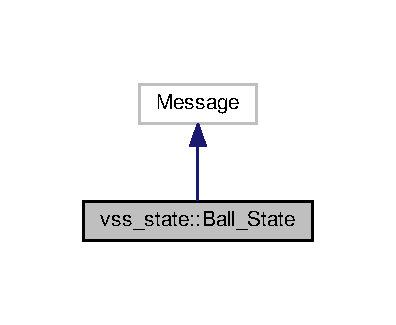
\includegraphics[width=190pt]{classvss__state_1_1Ball__State__inherit__graph}
\end{center}
\end{figure}


Collaboration diagram for vss\-\_\-state\-:\-:Ball\-\_\-\-State\-:
\nopagebreak
\begin{figure}[H]
\begin{center}
\leavevmode
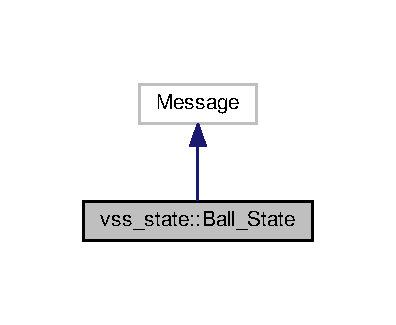
\includegraphics[width=190pt]{classvss__state_1_1Ball__State__coll__graph}
\end{center}
\end{figure}
\subsection*{Public Member Functions}
\begin{DoxyCompactItemize}
\item 
\hypertarget{classvss__state_1_1Ball__State_ac098b9cd5c2c3ddf8e51f0d2dbbf61fa}{{\bfseries Ball\-\_\-\-State} (const \hyperlink{classvss__state_1_1Ball__State}{Ball\-\_\-\-State} \&from)}\label{classvss__state_1_1Ball__State_ac098b9cd5c2c3ddf8e51f0d2dbbf61fa}

\item 
\hypertarget{classvss__state_1_1Ball__State_aa6cd23990f9da364b87df28c633d5935}{\hyperlink{classvss__state_1_1Ball__State}{Ball\-\_\-\-State} \& {\bfseries operator=} (const \hyperlink{classvss__state_1_1Ball__State}{Ball\-\_\-\-State} \&from)}\label{classvss__state_1_1Ball__State_aa6cd23990f9da364b87df28c633d5935}

\item 
\hypertarget{classvss__state_1_1Ball__State_a794e00572c1dadaee441bf94c11d7358}{const \\*
\-::google\-::protobuf\-::\-Unknown\-Field\-Set \& {\bfseries unknown\-\_\-fields} () const }\label{classvss__state_1_1Ball__State_a794e00572c1dadaee441bf94c11d7358}

\item 
\hypertarget{classvss__state_1_1Ball__State_a5d736fb563b0a4291d927a03394309b5}{inline\-::google\-::protobuf\-::\-Unknown\-Field\-Set $\ast$ {\bfseries mutable\-\_\-unknown\-\_\-fields} ()}\label{classvss__state_1_1Ball__State_a5d736fb563b0a4291d927a03394309b5}

\item 
\hypertarget{classvss__state_1_1Ball__State_a0e0face2c7b5e5b53793aa5e218a1623}{void {\bfseries Swap} (\hyperlink{classvss__state_1_1Ball__State}{Ball\-\_\-\-State} $\ast$other)}\label{classvss__state_1_1Ball__State_a0e0face2c7b5e5b53793aa5e218a1623}

\item 
\hypertarget{classvss__state_1_1Ball__State_a8788d4ca0089f7f0c043f5c763fee116}{\hyperlink{classvss__state_1_1Ball__State}{Ball\-\_\-\-State} $\ast$ {\bfseries New} () const }\label{classvss__state_1_1Ball__State_a8788d4ca0089f7f0c043f5c763fee116}

\item 
\hypertarget{classvss__state_1_1Ball__State_a1b6e1fc62b0ed7f4a56f51107c2dea0c}{void {\bfseries Copy\-From} (const \-::google\-::protobuf\-::\-Message \&from)}\label{classvss__state_1_1Ball__State_a1b6e1fc62b0ed7f4a56f51107c2dea0c}

\item 
\hypertarget{classvss__state_1_1Ball__State_a23b0aa5fb0ead3fa0eb1d49f044a4108}{void {\bfseries Merge\-From} (const \-::google\-::protobuf\-::\-Message \&from)}\label{classvss__state_1_1Ball__State_a23b0aa5fb0ead3fa0eb1d49f044a4108}

\item 
\hypertarget{classvss__state_1_1Ball__State_abc6d9bde7cd19d33f5592fe7e89958f2}{void {\bfseries Copy\-From} (const \hyperlink{classvss__state_1_1Ball__State}{Ball\-\_\-\-State} \&from)}\label{classvss__state_1_1Ball__State_abc6d9bde7cd19d33f5592fe7e89958f2}

\item 
\hypertarget{classvss__state_1_1Ball__State_a6c0a4da68998dea51ba4971d3f3ae758}{void {\bfseries Merge\-From} (const \hyperlink{classvss__state_1_1Ball__State}{Ball\-\_\-\-State} \&from)}\label{classvss__state_1_1Ball__State_a6c0a4da68998dea51ba4971d3f3ae758}

\item 
\hypertarget{classvss__state_1_1Ball__State_a23083679f69714534dff6d2fa4dfd69c}{void {\bfseries Clear} ()}\label{classvss__state_1_1Ball__State_a23083679f69714534dff6d2fa4dfd69c}

\item 
\hypertarget{classvss__state_1_1Ball__State_a86118bd22017a79d8bcecbb9759664ae}{bool {\bfseries Is\-Initialized} () const }\label{classvss__state_1_1Ball__State_a86118bd22017a79d8bcecbb9759664ae}

\item 
\hypertarget{classvss__state_1_1Ball__State_a37464e62ecce865fa9b7d71df18a6df2}{int {\bfseries Byte\-Size} () const }\label{classvss__state_1_1Ball__State_a37464e62ecce865fa9b7d71df18a6df2}

\item 
\hypertarget{classvss__state_1_1Ball__State_a23384562e9b1779b7eae6df07fec8c08}{bool {\bfseries Merge\-Partial\-From\-Coded\-Stream} (\-::google\-::protobuf\-::io\-::\-Coded\-Input\-Stream $\ast$input)}\label{classvss__state_1_1Ball__State_a23384562e9b1779b7eae6df07fec8c08}

\item 
\hypertarget{classvss__state_1_1Ball__State_ac9561ed1c347cc216c9adda156c8b1a7}{void {\bfseries Serialize\-With\-Cached\-Sizes} (\-::google\-::protobuf\-::io\-::\-Coded\-Output\-Stream $\ast$output) const }\label{classvss__state_1_1Ball__State_ac9561ed1c347cc216c9adda156c8b1a7}

\item 
\hypertarget{classvss__state_1_1Ball__State_a2db6bbee44c417e395cc2b707bbab23c}{\-::google\-::protobuf\-::uint8 $\ast$ {\bfseries Serialize\-With\-Cached\-Sizes\-To\-Array} (\-::google\-::protobuf\-::uint8 $\ast$output) const }\label{classvss__state_1_1Ball__State_a2db6bbee44c417e395cc2b707bbab23c}

\item 
\hypertarget{classvss__state_1_1Ball__State_a7f1be4451c61efb737a23f36191592f5}{int {\bfseries Get\-Cached\-Size} () const }\label{classvss__state_1_1Ball__State_a7f1be4451c61efb737a23f36191592f5}

\item 
\hypertarget{classvss__state_1_1Ball__State_ab93a553faefe3d3c98f56f6f84df0892}{\-::google\-::protobuf\-::\-Metadata {\bfseries Get\-Metadata} () const }\label{classvss__state_1_1Ball__State_ab93a553faefe3d3c98f56f6f84df0892}

\item 
\hypertarget{classvss__state_1_1Ball__State_a1108eb809324eb92f2bfeed247449ed4}{bool {\bfseries has\-\_\-x} () const }\label{classvss__state_1_1Ball__State_a1108eb809324eb92f2bfeed247449ed4}

\item 
\hypertarget{classvss__state_1_1Ball__State_abc5a7ab61fd68bb69f405160fb76dd2c}{void {\bfseries clear\-\_\-x} ()}\label{classvss__state_1_1Ball__State_abc5a7ab61fd68bb69f405160fb76dd2c}

\item 
\hypertarget{classvss__state_1_1Ball__State_a838cd2603deef45299fbea5bd36b5917}{float {\bfseries x} () const }\label{classvss__state_1_1Ball__State_a838cd2603deef45299fbea5bd36b5917}

\item 
\hypertarget{classvss__state_1_1Ball__State_a92bb7878b931bc72032adedb8ba094eb}{void {\bfseries set\-\_\-x} (float value)}\label{classvss__state_1_1Ball__State_a92bb7878b931bc72032adedb8ba094eb}

\item 
\hypertarget{classvss__state_1_1Ball__State_af3cd582b9e6429694e018d0a82a9a4c2}{bool {\bfseries has\-\_\-y} () const }\label{classvss__state_1_1Ball__State_af3cd582b9e6429694e018d0a82a9a4c2}

\item 
\hypertarget{classvss__state_1_1Ball__State_af9c47ba2a17c2e0e44d5e64e472336bc}{void {\bfseries clear\-\_\-y} ()}\label{classvss__state_1_1Ball__State_af9c47ba2a17c2e0e44d5e64e472336bc}

\item 
\hypertarget{classvss__state_1_1Ball__State_ac85ce8392a19e15e793ad7ab6140fb59}{float {\bfseries y} () const }\label{classvss__state_1_1Ball__State_ac85ce8392a19e15e793ad7ab6140fb59}

\item 
\hypertarget{classvss__state_1_1Ball__State_a590e0dd0fb1cbd600cf0bba31e9fa524}{void {\bfseries set\-\_\-y} (float value)}\label{classvss__state_1_1Ball__State_a590e0dd0fb1cbd600cf0bba31e9fa524}

\end{DoxyCompactItemize}
\subsection*{Static Public Member Functions}
\begin{DoxyCompactItemize}
\item 
\hypertarget{classvss__state_1_1Ball__State_adfc29a0088d19129c759d22494a74443}{static const \\*
\-::google\-::protobuf\-::\-Descriptor $\ast$ {\bfseries descriptor} ()}\label{classvss__state_1_1Ball__State_adfc29a0088d19129c759d22494a74443}

\item 
\hypertarget{classvss__state_1_1Ball__State_a762be08a3ad7dcbec17beb380b860f95}{static const \hyperlink{classvss__state_1_1Ball__State}{Ball\-\_\-\-State} \& {\bfseries default\-\_\-instance} ()}\label{classvss__state_1_1Ball__State_a762be08a3ad7dcbec17beb380b860f95}

\end{DoxyCompactItemize}
\subsection*{Static Public Attributes}
\begin{DoxyCompactItemize}
\item 
\hypertarget{classvss__state_1_1Ball__State_a35cabd2e3579b0e203e5acd1e77cfcad}{static const int {\bfseries k\-X\-Field\-Number} = 1}\label{classvss__state_1_1Ball__State_a35cabd2e3579b0e203e5acd1e77cfcad}

\item 
\hypertarget{classvss__state_1_1Ball__State_a70e818ce92aeb6531c7a163f1b0f2194}{static const int {\bfseries k\-Y\-Field\-Number} = 2}\label{classvss__state_1_1Ball__State_a70e818ce92aeb6531c7a163f1b0f2194}

\end{DoxyCompactItemize}
\subsection*{Friends}
\begin{DoxyCompactItemize}
\item 
\hypertarget{classvss__state_1_1Ball__State_aab1a2c258f8122a403a979ff57e2a706}{void {\bfseries protobuf\-\_\-\-Add\-Desc\-\_\-state\-\_\-2eproto} ()}\label{classvss__state_1_1Ball__State_aab1a2c258f8122a403a979ff57e2a706}

\item 
\hypertarget{classvss__state_1_1Ball__State_a57d9367bc8a7a94ead11d11194cca1b6}{void {\bfseries protobuf\-\_\-\-Assign\-Desc\-\_\-state\-\_\-2eproto} ()}\label{classvss__state_1_1Ball__State_a57d9367bc8a7a94ead11d11194cca1b6}

\item 
\hypertarget{classvss__state_1_1Ball__State_a4e6dc5e8e72799859c4e9556d090e57d}{void {\bfseries protobuf\-\_\-\-Shutdown\-File\-\_\-state\-\_\-2eproto} ()}\label{classvss__state_1_1Ball__State_a4e6dc5e8e72799859c4e9556d090e57d}

\end{DoxyCompactItemize}


The documentation for this class was generated from the following files\-:\begin{DoxyCompactItemize}
\item 
/home/oscar/\-Desktop/meu\-Fork/\-V\-S\-S-\/\-Vision/src/protos/state.\-pb.\-h\item 
/home/oscar/\-Desktop/meu\-Fork/\-V\-S\-S-\/\-Vision/src/protos/state.\-pb.\-cc\end{DoxyCompactItemize}

\hypertarget{structcommon_1_1btVector3}{}\section{common\+:\+:bt\+Vector3 Struct Reference}
\label{structcommon_1_1btVector3}\index{common\+::bt\+Vector3@{common\+::bt\+Vector3}}


This struct represents a Vector in R$^\wedge$3.  




{\ttfamily \#include $<$common.\+h$>$}

\subsection*{Public Member Functions}
\begin{DoxyCompactItemize}
\item 
\hyperlink{structcommon_1_1btVector3_a18054312f8905cc98697fe4b5918b92a}{bt\+Vector3} ()\hypertarget{structcommon_1_1btVector3_a18054312f8905cc98697fe4b5918b92a}{}\label{structcommon_1_1btVector3_a18054312f8905cc98697fe4b5918b92a}

\begin{DoxyCompactList}\small\item\em Default constructor\+: \hyperlink{structcommon_1_1btVector3}{bt\+Vector3} bt3;. \end{DoxyCompactList}\item 
\hyperlink{structcommon_1_1btVector3_a966ab1cbf7a9f4661ff9ab574466ad9f}{bt\+Vector3} (float \hyperlink{structcommon_1_1btVector3_adbe23ed6ae54734cbdf7b37788e0c702}{x}, float y, float z)\hypertarget{structcommon_1_1btVector3_a966ab1cbf7a9f4661ff9ab574466ad9f}{}\label{structcommon_1_1btVector3_a966ab1cbf7a9f4661ff9ab574466ad9f}

\begin{DoxyCompactList}\small\item\em Construtor X\+YZ\+: \hyperlink{structcommon_1_1btVector3}{bt\+Vector3} bt3(x, y, z);. \end{DoxyCompactList}\item 
\hyperlink{structcommon_1_1btVector3_aaed6af5e7b2e6217483dffa991ecffd4}{bt\+Vector3} (\hyperlink{structcommon_1_1btVector3}{bt\+Vector3} $\ast$b)\hypertarget{structcommon_1_1btVector3_aaed6af5e7b2e6217483dffa991ecffd4}{}\label{structcommon_1_1btVector3_aaed6af5e7b2e6217483dffa991ecffd4}

\begin{DoxyCompactList}\small\item\em Constructor copy\+: \hyperlink{structcommon_1_1btVector3}{bt\+Vector3} bt3(bt\+Vector3(x, y, z));. \end{DoxyCompactList}\item 
\hyperlink{structcommon_1_1btVector3_a276502eb04ec63d64566fa32c67f96fe}{bt\+Vector3} (Point $\ast$b)\hypertarget{structcommon_1_1btVector3_a276502eb04ec63d64566fa32c67f96fe}{}\label{structcommon_1_1btVector3_a276502eb04ec63d64566fa32c67f96fe}

\begin{DoxyCompactList}\small\item\em Constructor parse of point\+: \hyperlink{structcommon_1_1btVector3}{bt\+Vector3} bt3(\+Point(x, y));. \end{DoxyCompactList}\item 
void \hyperlink{structcommon_1_1btVector3_ad182266905d95459f9ca03da9af47f35}{show} ()\hypertarget{structcommon_1_1btVector3_ad182266905d95459f9ca03da9af47f35}{}\label{structcommon_1_1btVector3_ad182266905d95459f9ca03da9af47f35}

\begin{DoxyCompactList}\small\item\em Default function\+: prints all variables. \end{DoxyCompactList}\end{DoxyCompactItemize}
\subsection*{Public Attributes}
\begin{DoxyCompactItemize}
\item 
float \hyperlink{structcommon_1_1btVector3_adbe23ed6ae54734cbdf7b37788e0c702}{x}\hypertarget{structcommon_1_1btVector3_adbe23ed6ae54734cbdf7b37788e0c702}{}\label{structcommon_1_1btVector3_adbe23ed6ae54734cbdf7b37788e0c702}

\begin{DoxyCompactList}\small\item\em Data\+: x, y, z. \end{DoxyCompactList}\item 
float {\bfseries y}\hypertarget{structcommon_1_1btVector3_a5b52b09733d198cde3d283c0b2b320d1}{}\label{structcommon_1_1btVector3_a5b52b09733d198cde3d283c0b2b320d1}

\item 
float {\bfseries z}\hypertarget{structcommon_1_1btVector3_aa03665d96dd5d3dd2dbaeb6e9f24f4bc}{}\label{structcommon_1_1btVector3_aa03665d96dd5d3dd2dbaeb6e9f24f4bc}

\end{DoxyCompactItemize}


\subsection{Detailed Description}
This struct represents a Vector in R$^\wedge$3. 

The documentation for this struct was generated from the following file\+:\begin{DoxyCompactItemize}
\item 
/home/johnathan/\+Repositories/\+S\+I\+R\+Lab/\+V\+S\+S-\/\+Vision/master/src/common.\+h\end{DoxyCompactItemize}

\hypertarget{classcalibration}{}\section{calibration Class Reference}
\label{classcalibration}\index{calibration@{calibration}}


This class is responsible for calibrate all \hyperlink{structcommon_1_1VisionColor}{common\+::\+Vision\+Color}, cut points and rotation.  




{\ttfamily \#include $<$calibration.\+h$>$}



Inheritance diagram for calibration\+:
\nopagebreak
\begin{figure}[H]
\begin{center}
\leavevmode
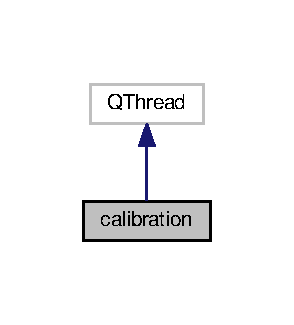
\includegraphics[width=141pt]{classcalibration__inherit__graph}
\end{center}
\end{figure}


Collaboration diagram for calibration\+:
\nopagebreak
\begin{figure}[H]
\begin{center}
\leavevmode
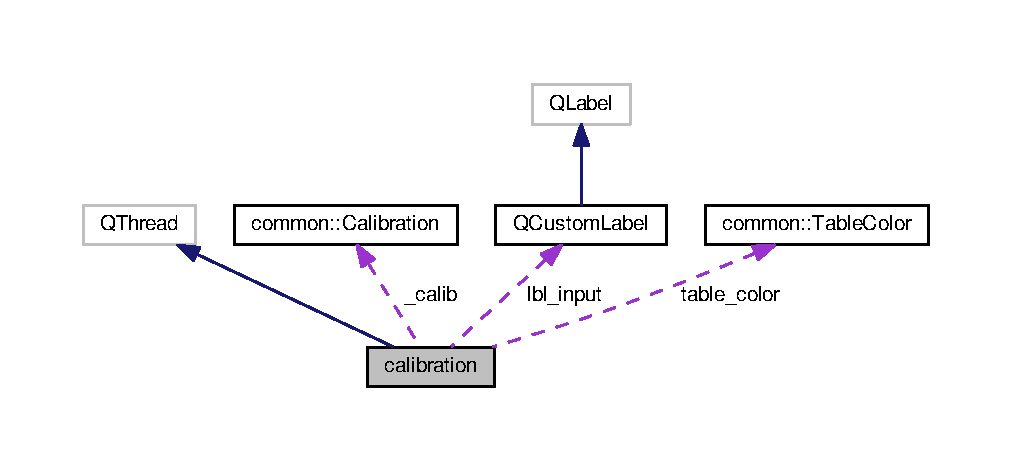
\includegraphics[width=350pt]{classcalibration__coll__graph}
\end{center}
\end{figure}
\subsection*{Signals}
\begin{DoxyCompactItemize}
\item 
void {\bfseries has\+\_\+new\+\_\+image} ()\hypertarget{classcalibration_a7e9eab43274288524d9d3c1a9d0f3b87}{}\label{classcalibration_a7e9eab43274288524d9d3c1a9d0f3b87}

\end{DoxyCompactItemize}
\subsection*{Public Member Functions}
\begin{DoxyCompactItemize}
\item 
\hyperlink{classcalibration_ad32a2ff0e4e27bd28ac06d7dda8b5853}{calibration} (Q\+Object $\ast$parent=0)
\begin{DoxyCompactList}\small\item\em Default constructor\+: calibration c;. \end{DoxyCompactList}\item 
void \hyperlink{classcalibration_a4b435b278f024e919b733627884ba0d2}{run} ()
\begin{DoxyCompactList}\small\item\em Virtual method from Q\+Thread, \hyperlink{classMainWindow}{Main\+Window} call this method in a C\+O\+N\+N\+E\+CT. \end{DoxyCompactList}\item 
void \hyperlink{classcalibration_a01c20860fb99a2370c191b0228e82af4}{finish} ()\hypertarget{classcalibration_a01c20860fb99a2370c191b0228e82af4}{}\label{classcalibration_a01c20860fb99a2370c191b0228e82af4}

\begin{DoxyCompactList}\small\item\em Virtual method from Q\+Thread, \hyperlink{classMainWindow}{Main\+Window} call this method in its destrcutor. \end{DoxyCompactList}\item 
void \hyperlink{classcalibration_a17edbce9454069eaa50cc84aa1cb34fd}{apply\+Filters} ()
\begin{DoxyCompactList}\small\item\em Apply all filters needed to find one blob. \end{DoxyCompactList}\item 
void \hyperlink{classcalibration_af2cc271619bd9d5c0e72ebbbf1b83f39}{zoom} ()
\begin{DoxyCompactList}\small\item\em Apply Zoom on image, if needed. \end{DoxyCompactList}\item 
void \hyperlink{classcalibration_a8beddb2a9ce3bef4dda101ea1f3f690c}{rotate\+\_\+image} ()\hypertarget{classcalibration_a8beddb2a9ce3bef4dda101ea1f3f690c}{}\label{classcalibration_a8beddb2a9ce3bef4dda101ea1f3f690c}

\begin{DoxyCompactList}\small\item\em rotate image \end{DoxyCompactList}\item 
void \hyperlink{classcalibration_ab1df3634bf6a485815310d1e2b7aa971}{cut\+\_\+image} ()\hypertarget{classcalibration_ab1df3634bf6a485815310d1e2b7aa971}{}\label{classcalibration_ab1df3634bf6a485815310d1e2b7aa971}

\begin{DoxyCompactList}\small\item\em cur image \end{DoxyCompactList}\item 
void \hyperlink{classcalibration_a9d29a622f2412fcf5cb654444d1bd43e}{paint\+\_\+output} ()
\begin{DoxyCompactList}\small\item\em Paint the blob founded. \end{DoxyCompactList}\item 
void \hyperlink{classcalibration_adba399584f906544ce09309e5539bb84}{set\+\_\+device} (int)\hypertarget{classcalibration_adba399584f906544ce09309e5539bb84}{}\label{classcalibration_adba399584f906544ce09309e5539bb84}

\begin{DoxyCompactList}\small\item\em Set the device time used, common\+::\+I\+M\+A\+GE, common\+::\+C\+A\+M\+E\+RA or common\+::\+V\+I\+D\+EO. \end{DoxyCompactList}\item 
void \hyperlink{classcalibration_aee45977e438474eb1111964a827a8ff9}{set\+\_\+id\+\_\+camera} (int)\hypertarget{classcalibration_aee45977e438474eb1111964a827a8ff9}{}\label{classcalibration_aee45977e438474eb1111964a827a8ff9}

\begin{DoxyCompactList}\small\item\em Set the id from camera used. \end{DoxyCompactList}\item 
void \hyperlink{classcalibration_a2eacc8d2c839f71182d3ec0440056ee7}{set\+\_\+path\+\_\+image} (string)\hypertarget{classcalibration_a2eacc8d2c839f71182d3ec0440056ee7}{}\label{classcalibration_a2eacc8d2c839f71182d3ec0440056ee7}

\begin{DoxyCompactList}\small\item\em Set the path of image used. \end{DoxyCompactList}\item 
void \hyperlink{classcalibration_ac4b64b95163be3bfdfb13c2d23592756}{set\+\_\+path\+\_\+video} (string)\hypertarget{classcalibration_ac4b64b95163be3bfdfb13c2d23592756}{}\label{classcalibration_ac4b64b95163be3bfdfb13c2d23592756}

\begin{DoxyCompactList}\small\item\em Set the path of video used. \end{DoxyCompactList}\item 
void \hyperlink{classcalibration_a5a1d0ee04511fc9a61767d3bb3f4e357}{set\+\_\+vision\+\_\+reception} (bool)
\begin{DoxyCompactList}\small\item\em Turn ON and O\+FF the vision reception and calcs. \end{DoxyCompactList}\item 
void \hyperlink{classcalibration_a6e2c50598a4f5d49c6d7bda23b69ddf3}{set\+\_\+id\+\_\+color} (int)\hypertarget{classcalibration_a6e2c50598a4f5d49c6d7bda23b69ddf3}{}\label{classcalibration_a6e2c50598a4f5d49c6d7bda23b69ddf3}

\begin{DoxyCompactList}\small\item\em Set the id\+\_\+color to calibrate, like\+: common\+::\+O\+R\+A\+N\+GE, common\+::\+Y\+E\+L\+L\+OW ... \end{DoxyCompactList}\item 
void \hyperlink{classcalibration_aaaf40baef708cb370c468ea0799ffaf6}{set\+\_\+mouse\+\_\+click\+\_\+left} (int)\hypertarget{classcalibration_aaaf40baef708cb370c468ea0799ffaf6}{}\label{classcalibration_aaaf40baef708cb370c468ea0799ffaf6}

\begin{DoxyCompactList}\small\item\em Set the qtd of left clicks. \end{DoxyCompactList}\item 
void \hyperlink{classcalibration_a788f9207f8641b1c3d3a74760e636bb3}{set\+\_\+mouse\+\_\+click\+\_\+right} (int)\hypertarget{classcalibration_a788f9207f8641b1c3d3a74760e636bb3}{}\label{classcalibration_a788f9207f8641b1c3d3a74760e636bb3}

\begin{DoxyCompactList}\small\item\em Set the qtd of right clicks. \end{DoxyCompactList}\item 
void \hyperlink{classcalibration_a7338523745caefc4ce7c156b5c52108f}{set\+\_\+type\+\_\+calibration} (bool)\hypertarget{classcalibration_a7338523745caefc4ce7c156b5c52108f}{}\label{classcalibration_a7338523745caefc4ce7c156b5c52108f}

\begin{DoxyCompactList}\small\item\em Set the type of calibration, C\+O\+L\+O\+RS = true, C\+AM = false;. \end{DoxyCompactList}\item 
int \hyperlink{classcalibration_a4c62df2cfea03276dde05134fd234b2c}{get\+\_\+device} ()\hypertarget{classcalibration_a4c62df2cfea03276dde05134fd234b2c}{}\label{classcalibration_a4c62df2cfea03276dde05134fd234b2c}

\begin{DoxyCompactList}\small\item\em get the device used \end{DoxyCompactList}\item 
int \hyperlink{classcalibration_a94b344ed8858fcb8509ba313d101d9c2}{get\+\_\+id\+\_\+camera} ()\hypertarget{classcalibration_a94b344ed8858fcb8509ba313d101d9c2}{}\label{classcalibration_a94b344ed8858fcb8509ba313d101d9c2}

\begin{DoxyCompactList}\small\item\em get the id from camera used \end{DoxyCompactList}\item 
string \hyperlink{classcalibration_aa607fee8c37d34cf3d812063ca7fb626}{get\+\_\+path\+\_\+image} ()\hypertarget{classcalibration_aa607fee8c37d34cf3d812063ca7fb626}{}\label{classcalibration_aa607fee8c37d34cf3d812063ca7fb626}

\begin{DoxyCompactList}\small\item\em get the path of image used \end{DoxyCompactList}\item 
bool \hyperlink{classcalibration_a567ceb5a68243624b3240955fdbfc50e}{get\+\_\+vision\+\_\+reception} ()\hypertarget{classcalibration_a567ceb5a68243624b3240955fdbfc50e}{}\label{classcalibration_a567ceb5a68243624b3240955fdbfc50e}

\begin{DoxyCompactList}\small\item\em get the path of video used \end{DoxyCompactList}\item 
int \hyperlink{classcalibration_a284e8a7b65d67601bd8d7bef949524df}{get\+\_\+id\+\_\+color} ()\hypertarget{classcalibration_a284e8a7b65d67601bd8d7bef949524df}{}\label{classcalibration_a284e8a7b65d67601bd8d7bef949524df}

\begin{DoxyCompactList}\small\item\em get the id color calibrate \end{DoxyCompactList}\item 
int \hyperlink{classcalibration_a45d0e76b3f360c7b198166cf7ccc638d}{get\+\_\+mouse\+\_\+click\+\_\+left} ()\hypertarget{classcalibration_a45d0e76b3f360c7b198166cf7ccc638d}{}\label{classcalibration_a45d0e76b3f360c7b198166cf7ccc638d}

\begin{DoxyCompactList}\small\item\em get the qtd of left clicks \end{DoxyCompactList}\item 
int \hyperlink{classcalibration_a8053c43e483faf127e20e16ff4ee6d8a}{get\+\_\+mouse\+\_\+click\+\_\+right} ()\hypertarget{classcalibration_a8053c43e483faf127e20e16ff4ee6d8a}{}\label{classcalibration_a8053c43e483faf127e20e16ff4ee6d8a}

\begin{DoxyCompactList}\small\item\em get the qtd of right clicks \end{DoxyCompactList}\item 
bool \hyperlink{classcalibration_ad22a724d4112abcb09ad8624e8b7d884}{get\+\_\+type\+\_\+calibration} ()\hypertarget{classcalibration_ad22a724d4112abcb09ad8624e8b7d884}{}\label{classcalibration_ad22a724d4112abcb09ad8624e8b7d884}

\begin{DoxyCompactList}\small\item\em get the type of calibraiton, C\+O\+L\+O\+RS = true, C\+AM = false; \end{DoxyCompactList}\item 
void \hyperlink{classcalibration_ab0b5f5514c665852aa63830121622518}{alloc\+\_\+label\+\_\+input} (\hyperlink{classQCustomLabel}{Q\+Custom\+Label} $\ast$)
\begin{DoxyCompactList}\small\item\em alloc the label of input image, image from Video\+Capture \end{DoxyCompactList}\item 
void \hyperlink{classcalibration_ac5e4cd1cead7176b0f34586112aaa918}{alloc\+\_\+calibration} (\hyperlink{structcommon_1_1Calibration}{Calibration} $\ast$)
\begin{DoxyCompactList}\small\item\em alloc the labels of pose from objects in workspace \end{DoxyCompactList}\end{DoxyCompactItemize}
\subsection*{Public Attributes}
\begin{DoxyCompactItemize}
\item 
Mat {\bfseries in}\hypertarget{classcalibration_a5381436b7a018d1bd969198a6ee84309}{}\label{classcalibration_a5381436b7a018d1bd969198a6ee84309}

\item 
Mat {\bfseries out}\hypertarget{classcalibration_a683520c2e997f8acf95d0c3cad6290b9}{}\label{classcalibration_a683520c2e997f8acf95d0c3cad6290b9}

\item 
Mat {\bfseries saved}\hypertarget{classcalibration_a992ee8c844d808217befd60c10c02980}{}\label{classcalibration_a992ee8c844d808217befd60c10c02980}

\item 
Mat {\bfseries raw\+\_\+in}\hypertarget{classcalibration_aa72b48a8e046d6409517e418335fb45b}{}\label{classcalibration_aa72b48a8e046d6409517e418335fb45b}

\item 
Mat {\bfseries raw\+\_\+out}\hypertarget{classcalibration_af12fa7781d0b718f408b6cae7a25704e}{}\label{classcalibration_af12fa7781d0b718f408b6cae7a25704e}

\item 
Mat {\bfseries storage}\hypertarget{classcalibration_a6eab74dcffae5bd8449df9b79b2d8ebc}{}\label{classcalibration_a6eab74dcffae5bd8449df9b79b2d8ebc}

\item 
Mat {\bfseries last\+\_\+in}\hypertarget{classcalibration_ad75ae06ee7d980f69ba065a8d8ddb574}{}\label{classcalibration_ad75ae06ee7d980f69ba065a8d8ddb574}

\end{DoxyCompactItemize}
\subsection*{Protected Attributes}
\begin{DoxyCompactItemize}
\item 
bool {\bfseries run\+\_\+it}\hypertarget{classcalibration_a3b4703e9670b0c80359bae2747878245}{}\label{classcalibration_a3b4703e9670b0c80359bae2747878245}

\item 
int {\bfseries device\+\_\+used}\hypertarget{classcalibration_a5f6ca76dc8c0fbf33f1c6a604b72cdc0}{}\label{classcalibration_a5f6ca76dc8c0fbf33f1c6a604b72cdc0}

\item 
bool {\bfseries vision\+\_\+reception}\hypertarget{classcalibration_a9606829157d28f46f87febceb67ba14c}{}\label{classcalibration_a9606829157d28f46f87febceb67ba14c}

\item 
bool {\bfseries start\+\_\+finish}\hypertarget{classcalibration_aa3b093eb7694fdcb78408efdeb331e01}{}\label{classcalibration_aa3b093eb7694fdcb78408efdeb331e01}

\item 
int {\bfseries id\+\_\+camera}\hypertarget{classcalibration_abb71e83b1caac73be1f8a5ec9ff85f5f}{}\label{classcalibration_abb71e83b1caac73be1f8a5ec9ff85f5f}

\item 
string {\bfseries user\+\_\+path}\hypertarget{classcalibration_a5e02265737a63f54063be406ab043a9e}{}\label{classcalibration_a5e02265737a63f54063be406ab043a9e}

\item 
string {\bfseries path\+\_\+image}\hypertarget{classcalibration_ab5b38c34686e2d0ef790f5ea1bf022d2}{}\label{classcalibration_ab5b38c34686e2d0ef790f5ea1bf022d2}

\item 
string {\bfseries path\+\_\+video}\hypertarget{classcalibration_ac3b22d58acc42fb7c8217518f6ea4846}{}\label{classcalibration_ac3b22d58acc42fb7c8217518f6ea4846}

\item 
int {\bfseries mouse\+\_\+click\+\_\+left}\hypertarget{classcalibration_ada27036ba780db458e9dc14f13f0809a}{}\label{classcalibration_ada27036ba780db458e9dc14f13f0809a}

\item 
int {\bfseries mouse\+\_\+click\+\_\+right}\hypertarget{classcalibration_a40702565952927ef98184ddeb27d5581}{}\label{classcalibration_a40702565952927ef98184ddeb27d5581}

\item 
int {\bfseries id\+\_\+calib}\hypertarget{classcalibration_a574fce12317e7968bd7553fbf715ab64}{}\label{classcalibration_a574fce12317e7968bd7553fbf715ab64}

\item 
bool {\bfseries type\+\_\+calibration}\hypertarget{classcalibration_a163c467c5b9ff3c58af7b443e2672cae}{}\label{classcalibration_a163c467c5b9ff3c58af7b443e2672cae}

\item 
Point {\bfseries size}\hypertarget{classcalibration_a10327f11f7951f4282ada6c354e62522}{}\label{classcalibration_a10327f11f7951f4282ada6c354e62522}

\item 
Video\+Capture {\bfseries cap}\hypertarget{classcalibration_a4fbb8e4cac6239dc7135963c0f500105}{}\label{classcalibration_a4fbb8e4cac6239dc7135963c0f500105}

\item 
vector$<$ vector$<$ Point $>$ $>$ {\bfseries labels}\hypertarget{classcalibration_ac1a1606070bf5b667f1e7a07e3e08d1d}{}\label{classcalibration_ac1a1606070bf5b667f1e7a07e3e08d1d}

\item 
vector$<$ vector$<$ Point $>$ $>$ {\bfseries contours}\hypertarget{classcalibration_a81c7edbfe89f8f1692193bc81309a55d}{}\label{classcalibration_a81c7edbfe89f8f1692193bc81309a55d}

\item 
vector$<$ Vec4i $>$ {\bfseries hierarchy}\hypertarget{classcalibration_a818940843ae109ee2e7bd3cb202c4704}{}\label{classcalibration_a818940843ae109ee2e7bd3cb202c4704}

\item 
Point {\bfseries zoom\+\_\+blob}\hypertarget{classcalibration_af15b11ca11726a106ce3581d28ae2fe2}{}\label{classcalibration_af15b11ca11726a106ce3581d28ae2fe2}

\item 
Q\+Image {\bfseries img}\hypertarget{classcalibration_abb31447445117b52af6865628355a76a}{}\label{classcalibration_abb31447445117b52af6865628355a76a}

\item 
\hyperlink{classQCustomLabel}{Q\+Custom\+Label} $\ast$ {\bfseries lbl\+\_\+input}\hypertarget{classcalibration_ade63c6e2fc49e68c15514133f30cbc65}{}\label{classcalibration_ade63c6e2fc49e68c15514133f30cbc65}

\item 
\hyperlink{structcommon_1_1Calibration}{Calibration} $\ast$ {\bfseries \+\_\+calib}\hypertarget{classcalibration_ad523b82addd861c31202b3d0d152f848}{}\label{classcalibration_ad523b82addd861c31202b3d0d152f848}

\item 
\hyperlink{structcommon_1_1TableColor}{Table\+Color} {\bfseries table\+\_\+color}\hypertarget{classcalibration_a941d98916460576b4bb2bfe9dd7c8f85}{}\label{classcalibration_a941d98916460576b4bb2bfe9dd7c8f85}

\end{DoxyCompactItemize}


\subsection{Detailed Description}
This class is responsible for calibrate all \hyperlink{structcommon_1_1VisionColor}{common\+::\+Vision\+Color}, cut points and rotation. 

\subsection{Constructor \& Destructor Documentation}
\index{calibration@{calibration}!calibration@{calibration}}
\index{calibration@{calibration}!calibration@{calibration}}
\subsubsection[{\texorpdfstring{calibration(\+Q\+Object $\ast$parent=0)}{calibration(QObject *parent=0)}}]{\setlength{\rightskip}{0pt plus 5cm}calibration\+::calibration (
\begin{DoxyParamCaption}
\item[{Q\+Object $\ast$}]{parent = {\ttfamily 0}}
\end{DoxyParamCaption}
)\hspace{0.3cm}{\ttfamily [explicit]}}\hypertarget{classcalibration_ad32a2ff0e4e27bd28ac06d7dda8b5853}{}\label{classcalibration_ad32a2ff0e4e27bd28ac06d7dda8b5853}


Default constructor\+: calibration c;. 

\subsubsection*{Addendum }

\begin{quote}
Initializes all control variables \end{quote}


\subsection{Member Function Documentation}
\index{calibration@{calibration}!alloc\+\_\+calibration@{alloc\+\_\+calibration}}
\index{alloc\+\_\+calibration@{alloc\+\_\+calibration}!calibration@{calibration}}
\subsubsection[{\texorpdfstring{alloc\+\_\+calibration(\+Calibration $\ast$)}{alloc_calibration(Calibration *)}}]{\setlength{\rightskip}{0pt plus 5cm}void calibration\+::alloc\+\_\+calibration (
\begin{DoxyParamCaption}
\item[{{\bf Calibration} $\ast$}]{\+\_\+calib}
\end{DoxyParamCaption}
)}\hypertarget{classcalibration_ac5e4cd1cead7176b0f34586112aaa918}{}\label{classcalibration_ac5e4cd1cead7176b0f34586112aaa918}


alloc the labels of pose from objects in workspace 

\subsubsection*{Addendum }\begin{quote}
It must be pointer, because calibration it\textquotesingle{}s unrecheable and \hyperlink{classMainWindow}{Main\+Window} too. \end{quote}
\index{calibration@{calibration}!alloc\+\_\+label\+\_\+input@{alloc\+\_\+label\+\_\+input}}
\index{alloc\+\_\+label\+\_\+input@{alloc\+\_\+label\+\_\+input}!calibration@{calibration}}
\subsubsection[{\texorpdfstring{alloc\+\_\+label\+\_\+input(\+Q\+Custom\+Label $\ast$)}{alloc_label_input(QCustomLabel *)}}]{\setlength{\rightskip}{0pt plus 5cm}void calibration\+::alloc\+\_\+label\+\_\+input (
\begin{DoxyParamCaption}
\item[{{\bf Q\+Custom\+Label} $\ast$}]{lbl\+\_\+input}
\end{DoxyParamCaption}
)}\hypertarget{classcalibration_ab0b5f5514c665852aa63830121622518}{}\label{classcalibration_ab0b5f5514c665852aa63830121622518}


alloc the label of input image, image from Video\+Capture 

\subsubsection*{Addendum }\begin{quote}
It must be pointer, because calibration it\textquotesingle{}s unrecheable and \hyperlink{classMainWindow}{Main\+Window} too. \end{quote}
\index{calibration@{calibration}!apply\+Filters@{apply\+Filters}}
\index{apply\+Filters@{apply\+Filters}!calibration@{calibration}}
\subsubsection[{\texorpdfstring{apply\+Filters()}{applyFilters()}}]{\setlength{\rightskip}{0pt plus 5cm}void calibration\+::apply\+Filters (
\begin{DoxyParamCaption}
{}
\end{DoxyParamCaption}
)}\hypertarget{classcalibration_a17edbce9454069eaa50cc84aa1cb34fd}{}\label{classcalibration_a17edbce9454069eaa50cc84aa1cb34fd}


Apply all filters needed to find one blob. 

\subsubsection*{Addendum }\begin{quote}
convert image, R\+GB -\/$>$ H\+SV \end{quote}


\begin{quote}
get the blobs \end{quote}


\begin{quote}
filter very small blobs \end{quote}


\begin{quote}
find the contour of all blobs \end{quote}


\begin{quote}
paint all blobs \end{quote}


\begin{quote}
Draw a with rectangle on all blobs \end{quote}
\index{calibration@{calibration}!paint\+\_\+output@{paint\+\_\+output}}
\index{paint\+\_\+output@{paint\+\_\+output}!calibration@{calibration}}
\subsubsection[{\texorpdfstring{paint\+\_\+output()}{paint_output()}}]{\setlength{\rightskip}{0pt plus 5cm}void calibration\+::paint\+\_\+output (
\begin{DoxyParamCaption}
{}
\end{DoxyParamCaption}
)}\hypertarget{classcalibration_a9d29a622f2412fcf5cb654444d1bd43e}{}\label{classcalibration_a9d29a622f2412fcf5cb654444d1bd43e}


Paint the blob founded. 

\subsubsection*{Addendum }\begin{quote}
If the H\+SV values its on range, paint with color\+: \hyperlink{structcommon_1_1TableColor}{common\+::\+Table\+Color}. \end{quote}
\index{calibration@{calibration}!run@{run}}
\index{run@{run}!calibration@{calibration}}
\subsubsection[{\texorpdfstring{run()}{run()}}]{\setlength{\rightskip}{0pt plus 5cm}void calibration\+::run (
\begin{DoxyParamCaption}
{}
\end{DoxyParamCaption}
)}\hypertarget{classcalibration_a4b435b278f024e919b733627884ba0d2}{}\label{classcalibration_a4b435b278f024e919b733627884ba0d2}


Virtual method from Q\+Thread, \hyperlink{classMainWindow}{Main\+Window} call this method in a C\+O\+N\+N\+E\+CT. 

\subsubsection*{Addendum }

\begin{quote}
loop from thread calibration \end{quote}
\begin{quote}
load the saved image \end{quote}


\begin{quote}
default imagem, blue screen \end{quote}


\begin{quote}
set the screen on \hyperlink{classMainWindow}{Main\+Window} \end{quote}


\begin{quote}
If vision reception must be used \end{quote}


Check devices and get image from them

\begin{quote}
if I\+M\+A\+GE it\textquotesingle{}s used, usleep(33333) its needed to limit fps in 30. \end{quote}


\begin{quote}
if V\+I\+D\+EO it\textquotesingle{}s used, and the video end, we reinititialize it \end{quote}


\begin{quote}
if V\+I\+D\+EO it\textquotesingle{}s used, usleep(33333) it\textquotesingle{}s needed to limit fps in 30 \end{quote}


\begin{quote}
Apply filters \end{quote}


\begin{quote}
Apply Zoom, if needed \end{quote}


\begin{quote}
emit a signal for \hyperlink{classMainWindow}{Main\+Window} update its image \end{quote}


\begin{quote}
If the vision reception was set false, we set the blue screen and release cv\+::\+Video\+Capture \end{quote}


\begin{quote}
If the vision reception it\textquotesingle{}s false, usleep(100000) to relieve the C\+PU \end{quote}
\index{calibration@{calibration}!set\+\_\+vision\+\_\+reception@{set\+\_\+vision\+\_\+reception}}
\index{set\+\_\+vision\+\_\+reception@{set\+\_\+vision\+\_\+reception}!calibration@{calibration}}
\subsubsection[{\texorpdfstring{set\+\_\+vision\+\_\+reception(bool)}{set_vision_reception(bool)}}]{\setlength{\rightskip}{0pt plus 5cm}void calibration\+::set\+\_\+vision\+\_\+reception (
\begin{DoxyParamCaption}
\item[{bool}]{}
\end{DoxyParamCaption}
)}\hypertarget{classcalibration_a5a1d0ee04511fc9a61767d3bb3f4e357}{}\label{classcalibration_a5a1d0ee04511fc9a61767d3bb3f4e357}


Turn ON and O\+FF the vision reception and calcs. 

\subsubsection*{Addendum }\begin{quote}
If device\+\_\+used == common\+::\+C\+A\+M\+E\+RA or common\+::\+V\+I\+D\+EO, start de Video\+Capture \end{quote}
\index{calibration@{calibration}!zoom@{zoom}}
\index{zoom@{zoom}!calibration@{calibration}}
\subsubsection[{\texorpdfstring{zoom()}{zoom()}}]{\setlength{\rightskip}{0pt plus 5cm}void calibration\+::zoom (
\begin{DoxyParamCaption}
{}
\end{DoxyParamCaption}
)}\hypertarget{classcalibration_af2cc271619bd9d5c0e72ebbbf1b83f39}{}\label{classcalibration_af2cc271619bd9d5c0e72ebbbf1b83f39}


Apply Zoom on image, if needed. 

\subsubsection*{Addendum }\begin{quote}
If the user click one time, the zoom it\textquotesingle{}s turned on If the user click one second time, the zoom it\textquotesingle{}s turned off \end{quote}


\begin{quote}
security, prevents that the zoom get out of image \end{quote}


\begin{quote}
security, prevents that the zoom get out of image \end{quote}


\begin{quote}
security, prevents that the zoom get out of image \end{quote}


\begin{quote}
security, prevents that the zoom get out of image \end{quote}


\begin{quote}
Apply de Zoom \end{quote}


\begin{quote}
Restart de count of clicks \end{quote}


The documentation for this class was generated from the following files\+:\begin{DoxyCompactItemize}
\item 
/home/johnathan/\+Repositories/\+S\+I\+R\+Lab/\+V\+S\+S-\/\+Vision/src/calibration.\+h\item 
/home/johnathan/\+Repositories/\+S\+I\+R\+Lab/\+V\+S\+S-\/\+Vision/src/calibration.\+cpp\end{DoxyCompactItemize}

\hypertarget{structcommon_1_1Calibration}{\section{common\-:\-:Calibration Struct Reference}
\label{structcommon_1_1Calibration}\index{common\-::\-Calibration@{common\-::\-Calibration}}
}


This struct represents a calibration of colors.  




{\ttfamily \#include $<$common.\-h$>$}

\subsection*{Public Member Functions}
\begin{DoxyCompactItemize}
\item 
\hypertarget{structcommon_1_1Calibration_a5c5c85c1e1ff7b5f1e5272deb8bf04b2}{\hyperlink{structcommon_1_1Calibration_a5c5c85c1e1ff7b5f1e5272deb8bf04b2}{Calibration} ()}\label{structcommon_1_1Calibration_a5c5c85c1e1ff7b5f1e5272deb8bf04b2}

\begin{DoxyCompactList}\small\item\em Default constructor\-: \hyperlink{structcommon_1_1Calibration}{Calibration} c; initialize the vector with range of colors in H\-S\-V to track the objects with Saved Video and Saved Image. \end{DoxyCompactList}\item 
\hypertarget{structcommon_1_1Calibration_a4c79aae796dd932808e8e009643164d7}{\hyperlink{structcommon_1_1Calibration_a4c79aae796dd932808e8e009643164d7}{Calibration} (\hyperlink{structcommon_1_1Calibration}{Calibration} $\ast$c)}\label{structcommon_1_1Calibration_a4c79aae796dd932808e8e009643164d7}

\begin{DoxyCompactList}\small\item\em Constructor copy\-: \hyperlink{structcommon_1_1Calibration}{Calibration} c(\-Calibration());. \end{DoxyCompactList}\item 
\hypertarget{structcommon_1_1Calibration_aaec2830170bbb7dbce05c9e3139549a6}{void \hyperlink{structcommon_1_1Calibration_aaec2830170bbb7dbce05c9e3139549a6}{show} ()}\label{structcommon_1_1Calibration_aaec2830170bbb7dbce05c9e3139549a6}

\begin{DoxyCompactList}\small\item\em Default function\-: prints all variables. \end{DoxyCompactList}\end{DoxyCompactItemize}
\subsection*{Public Attributes}
\begin{DoxyCompactItemize}
\item 
\hypertarget{structcommon_1_1Calibration_af7faad7cda5adfffefa44006cdecea85}{string \hyperlink{structcommon_1_1Calibration_af7faad7cda5adfffefa44006cdecea85}{comment}}\label{structcommon_1_1Calibration_af7faad7cda5adfffefa44006cdecea85}

\begin{DoxyCompactList}\small\item\em Data\-: comment of calibration. used to save in db. \end{DoxyCompactList}\item 
\hypertarget{structcommon_1_1Calibration_a219ffe804bda864b9757bc5d32ee49c4}{vector$<$ \hyperlink{structcommon_1_1VisionColor}{Vision\-Color} $>$ \hyperlink{structcommon_1_1Calibration_a219ffe804bda864b9757bc5d32ee49c4}{colors}}\label{structcommon_1_1Calibration_a219ffe804bda864b9757bc5d32ee49c4}

\begin{DoxyCompactList}\small\item\em Data\-: vector of \hyperlink{structcommon_1_1VisionColor}{Vision\-Color}. \end{DoxyCompactList}\item 
\hypertarget{structcommon_1_1Calibration_adb64222af92367a220f889876324edbc}{vector$<$ Point $>$ \hyperlink{structcommon_1_1Calibration_adb64222af92367a220f889876324edbc}{cut}}\label{structcommon_1_1Calibration_adb64222af92367a220f889876324edbc}

\begin{DoxyCompactList}\small\item\em Data\-: vector of Point. \end{DoxyCompactList}\item 
\hypertarget{structcommon_1_1Calibration_abd3a75564db014e04bf2ee76512a3f0b}{string \hyperlink{structcommon_1_1Calibration_abd3a75564db014e04bf2ee76512a3f0b}{data}}\label{structcommon_1_1Calibration_abd3a75564db014e04bf2ee76512a3f0b}

\begin{DoxyCompactList}\small\item\em Data\-: day of calibration. used ti save in db. \end{DoxyCompactList}\end{DoxyCompactItemize}


\subsection{Detailed Description}
This struct represents a calibration of colors. 

The documentation for this struct was generated from the following file\-:\begin{DoxyCompactItemize}
\item 
/home/oscar/\-Desktop/meu\-Fork/\-V\-S\-S-\/\-Vision/src/common.\-h\end{DoxyCompactItemize}

\hypertarget{structcommon_1_1ExecConfiguration}{}\section{common\+:\+:Exec\+Configuration Struct Reference}
\label{structcommon_1_1ExecConfiguration}\index{common\+::\+Exec\+Configuration@{common\+::\+Exec\+Configuration}}


This struct represents a configuration of colors of objects in workspace.  




{\ttfamily \#include $<$common.\+h$>$}

\subsection*{Public Member Functions}
\begin{DoxyCompactItemize}
\item 
\hyperlink{structcommon_1_1ExecConfiguration_ae71329df20ba52327f33287c50663ac1}{Exec\+Configuration} ()\hypertarget{structcommon_1_1ExecConfiguration_ae71329df20ba52327f33287c50663ac1}{}\label{structcommon_1_1ExecConfiguration_ae71329df20ba52327f33287c50663ac1}

\begin{DoxyCompactList}\small\item\em Default constructor\+: \hyperlink{structcommon_1_1ExecConfiguration}{Exec\+Configuration} exex;. \end{DoxyCompactList}\item 
\hyperlink{structcommon_1_1ExecConfiguration_acdd086538b27972751b0b18f78a45e01}{Exec\+Configuration} (\hyperlink{structcommon_1_1ExecConfiguration}{Exec\+Configuration} $\ast$g)\hypertarget{structcommon_1_1ExecConfiguration_acdd086538b27972751b0b18f78a45e01}{}\label{structcommon_1_1ExecConfiguration_acdd086538b27972751b0b18f78a45e01}

\begin{DoxyCompactList}\small\item\em Constructor copy\+: Exex\+Configuration exex(\+Exec\+Configuration());. \end{DoxyCompactList}\item 
void \hyperlink{structcommon_1_1ExecConfiguration_a428c6689fbc17376db7304dd61f3d69b}{show} ()\hypertarget{structcommon_1_1ExecConfiguration_a428c6689fbc17376db7304dd61f3d69b}{}\label{structcommon_1_1ExecConfiguration_a428c6689fbc17376db7304dd61f3d69b}

\begin{DoxyCompactList}\small\item\em Default function\+: prints all variables. \end{DoxyCompactList}\end{DoxyCompactItemize}
\subsection*{Public Attributes}
\begin{DoxyCompactItemize}
\item 
string \hyperlink{structcommon_1_1ExecConfiguration_a98f8739d11ff3ab4e9e6f61a1d8084a4}{comment}\hypertarget{structcommon_1_1ExecConfiguration_a98f8739d11ff3ab4e9e6f61a1d8084a4}{}\label{structcommon_1_1ExecConfiguration_a98f8739d11ff3ab4e9e6f61a1d8084a4}

\begin{DoxyCompactList}\small\item\em Data\+: comment of configuration. used to save in db. \end{DoxyCompactList}\item 
int \hyperlink{structcommon_1_1ExecConfiguration_a08b7bbd7185afc2f9050850771af86c8}{ball\+\_\+color}\hypertarget{structcommon_1_1ExecConfiguration_a08b7bbd7185afc2f9050850771af86c8}{}\label{structcommon_1_1ExecConfiguration_a08b7bbd7185afc2f9050850771af86c8}

\begin{DoxyCompactList}\small\item\em Data\+: E\+N\+UM id\+\_\+color. \end{DoxyCompactList}\item 
int \hyperlink{structcommon_1_1ExecConfiguration_a2f8748f7ea7c3b21a580b9116efc5593}{team\+\_\+color} \mbox{[}2\mbox{]}\hypertarget{structcommon_1_1ExecConfiguration_a2f8748f7ea7c3b21a580b9116efc5593}{}\label{structcommon_1_1ExecConfiguration_a2f8748f7ea7c3b21a580b9116efc5593}

\begin{DoxyCompactList}\small\item\em Data\+: E\+N\+UM id\+\_\+color. \end{DoxyCompactList}\item 
int \hyperlink{structcommon_1_1ExecConfiguration_aa8dcf45e57d1a2e2264d75e2568e33bf}{config\+\_\+labels} \mbox{[}2\mbox{]}\hypertarget{structcommon_1_1ExecConfiguration_aa8dcf45e57d1a2e2264d75e2568e33bf}{}\label{structcommon_1_1ExecConfiguration_aa8dcf45e57d1a2e2264d75e2568e33bf}

\begin{DoxyCompactList}\small\item\em Data\+: E\+N\+UM id\+\_\+color. \end{DoxyCompactList}\item 
int \hyperlink{structcommon_1_1ExecConfiguration_a5485a96fed9500bddfd4a8ce81d9032c}{secundary\+\_\+color\+\_\+1} \mbox{[}3\mbox{]}\hypertarget{structcommon_1_1ExecConfiguration_a5485a96fed9500bddfd4a8ce81d9032c}{}\label{structcommon_1_1ExecConfiguration_a5485a96fed9500bddfd4a8ce81d9032c}

\begin{DoxyCompactList}\small\item\em Data\+: E\+N\+UM id\+\_\+color. \end{DoxyCompactList}\item 
int \hyperlink{structcommon_1_1ExecConfiguration_aea1aed941fceb299c6766e6330ec802e}{secundary\+\_\+color\+\_\+2} \mbox{[}3\mbox{]}\hypertarget{structcommon_1_1ExecConfiguration_aea1aed941fceb299c6766e6330ec802e}{}\label{structcommon_1_1ExecConfiguration_aea1aed941fceb299c6766e6330ec802e}

\begin{DoxyCompactList}\small\item\em Data\+: E\+N\+UM id\+\_\+color. \end{DoxyCompactList}\end{DoxyCompactItemize}


\subsection{Detailed Description}
This struct represents a configuration of colors of objects in workspace. 

The documentation for this struct was generated from the following file\+:\begin{DoxyCompactItemize}
\item 
/home/johnathan/\+Repositories/\+S\+I\+R\+Lab/\+V\+S\+S-\/\+Vision/master/src/common.\+h\end{DoxyCompactItemize}

\hypertarget{classvss__command_1_1Global__Commands}{\section{vss\-\_\-command\-:\-:Global\-\_\-\-Commands Class Reference}
\label{classvss__command_1_1Global__Commands}\index{vss\-\_\-command\-::\-Global\-\_\-\-Commands@{vss\-\_\-command\-::\-Global\-\_\-\-Commands}}
}


Inheritance diagram for vss\-\_\-command\-:\-:Global\-\_\-\-Commands\-:
\nopagebreak
\begin{figure}[H]
\begin{center}
\leavevmode
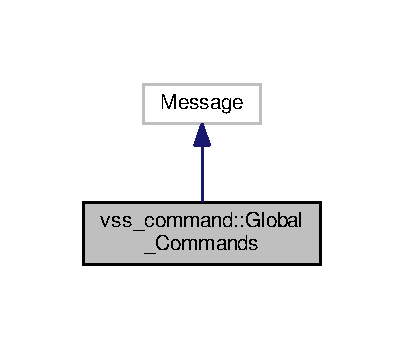
\includegraphics[width=194pt]{classvss__command_1_1Global__Commands__inherit__graph}
\end{center}
\end{figure}


Collaboration diagram for vss\-\_\-command\-:\-:Global\-\_\-\-Commands\-:
\nopagebreak
\begin{figure}[H]
\begin{center}
\leavevmode
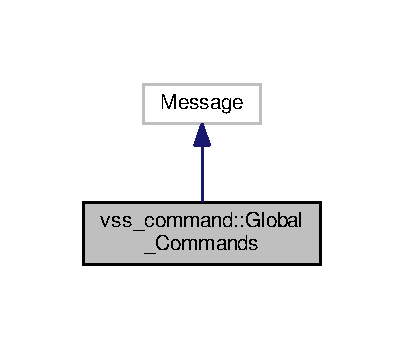
\includegraphics[width=194pt]{classvss__command_1_1Global__Commands__coll__graph}
\end{center}
\end{figure}
\subsection*{Public Member Functions}
\begin{DoxyCompactItemize}
\item 
\hypertarget{classvss__command_1_1Global__Commands_ac5a1e52df1880363fccb681c303ec821}{{\bfseries Global\-\_\-\-Commands} (const \hyperlink{classvss__command_1_1Global__Commands}{Global\-\_\-\-Commands} \&from)}\label{classvss__command_1_1Global__Commands_ac5a1e52df1880363fccb681c303ec821}

\item 
\hypertarget{classvss__command_1_1Global__Commands_a1e2590dfc4b0e2c8c20a8f5c68531a22}{\hyperlink{classvss__command_1_1Global__Commands}{Global\-\_\-\-Commands} \& {\bfseries operator=} (const \hyperlink{classvss__command_1_1Global__Commands}{Global\-\_\-\-Commands} \&from)}\label{classvss__command_1_1Global__Commands_a1e2590dfc4b0e2c8c20a8f5c68531a22}

\item 
\hypertarget{classvss__command_1_1Global__Commands_aadc4690c81ad4df3443b087428e1de73}{const \\*
\-::google\-::protobuf\-::\-Unknown\-Field\-Set \& {\bfseries unknown\-\_\-fields} () const }\label{classvss__command_1_1Global__Commands_aadc4690c81ad4df3443b087428e1de73}

\item 
\hypertarget{classvss__command_1_1Global__Commands_a1882397164e8072272d76b8172991013}{inline\-::google\-::protobuf\-::\-Unknown\-Field\-Set $\ast$ {\bfseries mutable\-\_\-unknown\-\_\-fields} ()}\label{classvss__command_1_1Global__Commands_a1882397164e8072272d76b8172991013}

\item 
\hypertarget{classvss__command_1_1Global__Commands_a1bf67bb767a2b899fceb94bf88a52ba7}{void {\bfseries Swap} (\hyperlink{classvss__command_1_1Global__Commands}{Global\-\_\-\-Commands} $\ast$other)}\label{classvss__command_1_1Global__Commands_a1bf67bb767a2b899fceb94bf88a52ba7}

\item 
\hypertarget{classvss__command_1_1Global__Commands_a6d4aeb9a55672fcfa0876e62de431a05}{\hyperlink{classvss__command_1_1Global__Commands}{Global\-\_\-\-Commands} $\ast$ {\bfseries New} () const }\label{classvss__command_1_1Global__Commands_a6d4aeb9a55672fcfa0876e62de431a05}

\item 
\hypertarget{classvss__command_1_1Global__Commands_a4bd5bb12d6e5f08346704aa04a30fe57}{void {\bfseries Copy\-From} (const \-::google\-::protobuf\-::\-Message \&from)}\label{classvss__command_1_1Global__Commands_a4bd5bb12d6e5f08346704aa04a30fe57}

\item 
\hypertarget{classvss__command_1_1Global__Commands_a70b24974df993bc6cd742f074555544b}{void {\bfseries Merge\-From} (const \-::google\-::protobuf\-::\-Message \&from)}\label{classvss__command_1_1Global__Commands_a70b24974df993bc6cd742f074555544b}

\item 
\hypertarget{classvss__command_1_1Global__Commands_a2c2be618a14de139a996c3f40cdcaa7c}{void {\bfseries Copy\-From} (const \hyperlink{classvss__command_1_1Global__Commands}{Global\-\_\-\-Commands} \&from)}\label{classvss__command_1_1Global__Commands_a2c2be618a14de139a996c3f40cdcaa7c}

\item 
\hypertarget{classvss__command_1_1Global__Commands_a72522cd185ed392c8dba2b746f1c10be}{void {\bfseries Merge\-From} (const \hyperlink{classvss__command_1_1Global__Commands}{Global\-\_\-\-Commands} \&from)}\label{classvss__command_1_1Global__Commands_a72522cd185ed392c8dba2b746f1c10be}

\item 
\hypertarget{classvss__command_1_1Global__Commands_a9027fa1a333a49d2a9e7927f1241d2d7}{void {\bfseries Clear} ()}\label{classvss__command_1_1Global__Commands_a9027fa1a333a49d2a9e7927f1241d2d7}

\item 
\hypertarget{classvss__command_1_1Global__Commands_ab59f63095dd243cd7311d9142a9326ef}{bool {\bfseries Is\-Initialized} () const }\label{classvss__command_1_1Global__Commands_ab59f63095dd243cd7311d9142a9326ef}

\item 
\hypertarget{classvss__command_1_1Global__Commands_a05036b0569ebf9d13ff9cee1430ffb12}{int {\bfseries Byte\-Size} () const }\label{classvss__command_1_1Global__Commands_a05036b0569ebf9d13ff9cee1430ffb12}

\item 
\hypertarget{classvss__command_1_1Global__Commands_a0d0fcd0747bad0226fb5a0829f45ed1b}{bool {\bfseries Merge\-Partial\-From\-Coded\-Stream} (\-::google\-::protobuf\-::io\-::\-Coded\-Input\-Stream $\ast$input)}\label{classvss__command_1_1Global__Commands_a0d0fcd0747bad0226fb5a0829f45ed1b}

\item 
\hypertarget{classvss__command_1_1Global__Commands_a35292dbb1e0ac73f11bedc01a64e751e}{void {\bfseries Serialize\-With\-Cached\-Sizes} (\-::google\-::protobuf\-::io\-::\-Coded\-Output\-Stream $\ast$output) const }\label{classvss__command_1_1Global__Commands_a35292dbb1e0ac73f11bedc01a64e751e}

\item 
\hypertarget{classvss__command_1_1Global__Commands_a124cdc7e8bf7200c9f11c801cbcaa9d4}{\-::google\-::protobuf\-::uint8 $\ast$ {\bfseries Serialize\-With\-Cached\-Sizes\-To\-Array} (\-::google\-::protobuf\-::uint8 $\ast$output) const }\label{classvss__command_1_1Global__Commands_a124cdc7e8bf7200c9f11c801cbcaa9d4}

\item 
\hypertarget{classvss__command_1_1Global__Commands_a87d23baa19f2c0272a75e15dfa234f08}{int {\bfseries Get\-Cached\-Size} () const }\label{classvss__command_1_1Global__Commands_a87d23baa19f2c0272a75e15dfa234f08}

\item 
\hypertarget{classvss__command_1_1Global__Commands_ae82e1f8fbfdf6f364c915da6d0e12f33}{\-::google\-::protobuf\-::\-Metadata {\bfseries Get\-Metadata} () const }\label{classvss__command_1_1Global__Commands_ae82e1f8fbfdf6f364c915da6d0e12f33}

\item 
\hypertarget{classvss__command_1_1Global__Commands_a70a923cca7611e0bd3c322a1ac5e91ba}{bool {\bfseries has\-\_\-id} () const }\label{classvss__command_1_1Global__Commands_a70a923cca7611e0bd3c322a1ac5e91ba}

\item 
\hypertarget{classvss__command_1_1Global__Commands_a32c51afe77b984a2be61e786893dd382}{void {\bfseries clear\-\_\-id} ()}\label{classvss__command_1_1Global__Commands_a32c51afe77b984a2be61e786893dd382}

\item 
\hypertarget{classvss__command_1_1Global__Commands_ac4b50f174ae21e1ef747b8d2498d9651}{inline\-::google\-::protobuf\-::uint32 {\bfseries id} () const }\label{classvss__command_1_1Global__Commands_ac4b50f174ae21e1ef747b8d2498d9651}

\item 
\hypertarget{classvss__command_1_1Global__Commands_aba49ba26507d3a54403584352f3dde90}{void {\bfseries set\-\_\-id} (\-::google\-::protobuf\-::uint32 value)}\label{classvss__command_1_1Global__Commands_aba49ba26507d3a54403584352f3dde90}

\item 
\hypertarget{classvss__command_1_1Global__Commands_a01e1a3bf6986a61900153eec4e51ac9b}{bool {\bfseries has\-\_\-is\-\_\-team\-\_\-yellow} () const }\label{classvss__command_1_1Global__Commands_a01e1a3bf6986a61900153eec4e51ac9b}

\item 
\hypertarget{classvss__command_1_1Global__Commands_ad626702bff23b842c6c342fb94ed9097}{void {\bfseries clear\-\_\-is\-\_\-team\-\_\-yellow} ()}\label{classvss__command_1_1Global__Commands_ad626702bff23b842c6c342fb94ed9097}

\item 
\hypertarget{classvss__command_1_1Global__Commands_a82e8f2fd24d0bcbf30e924d18dd8bba8}{bool {\bfseries is\-\_\-team\-\_\-yellow} () const }\label{classvss__command_1_1Global__Commands_a82e8f2fd24d0bcbf30e924d18dd8bba8}

\item 
\hypertarget{classvss__command_1_1Global__Commands_ac7855fe013be0c1be3f573a1b6eb47dc}{void {\bfseries set\-\_\-is\-\_\-team\-\_\-yellow} (bool value)}\label{classvss__command_1_1Global__Commands_ac7855fe013be0c1be3f573a1b6eb47dc}

\item 
\hypertarget{classvss__command_1_1Global__Commands_a09f12589e89e8d27a0e0d6fb7ecbcee3}{int {\bfseries robot\-\_\-commands\-\_\-size} () const }\label{classvss__command_1_1Global__Commands_a09f12589e89e8d27a0e0d6fb7ecbcee3}

\item 
\hypertarget{classvss__command_1_1Global__Commands_a2624ae56ed92fe0cf6617f8c740ad2d2}{void {\bfseries clear\-\_\-robot\-\_\-commands} ()}\label{classvss__command_1_1Global__Commands_a2624ae56ed92fe0cf6617f8c740ad2d2}

\item 
\hypertarget{classvss__command_1_1Global__Commands_aa6bd99500ef874f4a68cbf1adecf0fd1}{const \\*
\-::\hyperlink{classvss__command_1_1Robot__Command}{vss\-\_\-command\-::\-Robot\-\_\-\-Command} \& {\bfseries robot\-\_\-commands} (int index) const }\label{classvss__command_1_1Global__Commands_aa6bd99500ef874f4a68cbf1adecf0fd1}

\item 
\hypertarget{classvss__command_1_1Global__Commands_a08dc88b20105318b2cc8bbbbf2300581}{inline\-::vss\-\_\-command\-::\-Robot\-\_\-\-Command $\ast$ {\bfseries mutable\-\_\-robot\-\_\-commands} (int index)}\label{classvss__command_1_1Global__Commands_a08dc88b20105318b2cc8bbbbf2300581}

\item 
\hypertarget{classvss__command_1_1Global__Commands_add6abc22ca67ffa146cfba3e0b17ad2b}{inline\-::vss\-\_\-command\-::\-Robot\-\_\-\-Command $\ast$ {\bfseries add\-\_\-robot\-\_\-commands} ()}\label{classvss__command_1_1Global__Commands_add6abc22ca67ffa146cfba3e0b17ad2b}

\item 
\hypertarget{classvss__command_1_1Global__Commands_acb14464615fbad56ce9a1da3ce46373a}{const \\*
\-::google\-::protobuf\-::\-Repeated\-Ptr\-Field\\*
$<$ \-::\hyperlink{classvss__command_1_1Robot__Command}{vss\-\_\-command\-::\-Robot\-\_\-\-Command} $>$ \& {\bfseries robot\-\_\-commands} () const }\label{classvss__command_1_1Global__Commands_acb14464615fbad56ce9a1da3ce46373a}

\item 
\hypertarget{classvss__command_1_1Global__Commands_a3de88f16ed28f63fed38eff2ef169df4}{inline\-::google\-::protobuf\-::\-Repeated\-Ptr\-Field\\*
$<$ \-::\hyperlink{classvss__command_1_1Robot__Command}{vss\-\_\-command\-::\-Robot\-\_\-\-Command} $>$ $\ast$ {\bfseries mutable\-\_\-robot\-\_\-commands} ()}\label{classvss__command_1_1Global__Commands_a3de88f16ed28f63fed38eff2ef169df4}

\end{DoxyCompactItemize}
\subsection*{Static Public Member Functions}
\begin{DoxyCompactItemize}
\item 
\hypertarget{classvss__command_1_1Global__Commands_a26e4245a80fa599d0e30613122af7ad9}{static const \\*
\-::google\-::protobuf\-::\-Descriptor $\ast$ {\bfseries descriptor} ()}\label{classvss__command_1_1Global__Commands_a26e4245a80fa599d0e30613122af7ad9}

\item 
\hypertarget{classvss__command_1_1Global__Commands_a9e44db388aae4a529e0bff71979eea66}{static const \hyperlink{classvss__command_1_1Global__Commands}{Global\-\_\-\-Commands} \& {\bfseries default\-\_\-instance} ()}\label{classvss__command_1_1Global__Commands_a9e44db388aae4a529e0bff71979eea66}

\end{DoxyCompactItemize}
\subsection*{Static Public Attributes}
\begin{DoxyCompactItemize}
\item 
\hypertarget{classvss__command_1_1Global__Commands_a67c9ce208f0648844211d1faca128e34}{static const int {\bfseries k\-Id\-Field\-Number} = 1}\label{classvss__command_1_1Global__Commands_a67c9ce208f0648844211d1faca128e34}

\item 
\hypertarget{classvss__command_1_1Global__Commands_a90443d587b7a5171b061ec96660b04ef}{static const int {\bfseries k\-Is\-Team\-Yellow\-Field\-Number} = 2}\label{classvss__command_1_1Global__Commands_a90443d587b7a5171b061ec96660b04ef}

\item 
\hypertarget{classvss__command_1_1Global__Commands_a65b203ec091ad5cce5fcb7b34b01bcf1}{static const int {\bfseries k\-Robot\-Commands\-Field\-Number} = 3}\label{classvss__command_1_1Global__Commands_a65b203ec091ad5cce5fcb7b34b01bcf1}

\end{DoxyCompactItemize}
\subsection*{Friends}
\begin{DoxyCompactItemize}
\item 
\hypertarget{classvss__command_1_1Global__Commands_a4825d92f856fcb4b02c67b601c433796}{void {\bfseries protobuf\-\_\-\-Add\-Desc\-\_\-command\-\_\-2eproto} ()}\label{classvss__command_1_1Global__Commands_a4825d92f856fcb4b02c67b601c433796}

\item 
\hypertarget{classvss__command_1_1Global__Commands_a4c6fb97c25079d49daf010087d869100}{void {\bfseries protobuf\-\_\-\-Assign\-Desc\-\_\-command\-\_\-2eproto} ()}\label{classvss__command_1_1Global__Commands_a4c6fb97c25079d49daf010087d869100}

\item 
\hypertarget{classvss__command_1_1Global__Commands_a4cf10633ad46690f5eec6bdbbcf62de0}{void {\bfseries protobuf\-\_\-\-Shutdown\-File\-\_\-command\-\_\-2eproto} ()}\label{classvss__command_1_1Global__Commands_a4cf10633ad46690f5eec6bdbbcf62de0}

\end{DoxyCompactItemize}


The documentation for this class was generated from the following files\-:\begin{DoxyCompactItemize}
\item 
/home/oscar/\-Desktop/meu\-Fork/\-V\-S\-S-\/\-Vision/src/protos/command.\-pb.\-h\item 
/home/oscar/\-Desktop/meu\-Fork/\-V\-S\-S-\/\-Vision/src/protos/command.\-pb.\-cc\end{DoxyCompactItemize}

\hypertarget{classvss__state_1_1Global__State}{}\section{vss\+\_\+state\+:\+:Global\+\_\+\+State Class Reference}
\label{classvss__state_1_1Global__State}\index{vss\+\_\+state\+::\+Global\+\_\+\+State@{vss\+\_\+state\+::\+Global\+\_\+\+State}}


Inheritance diagram for vss\+\_\+state\+:\+:Global\+\_\+\+State\+:
\nopagebreak
\begin{figure}[H]
\begin{center}
\leavevmode
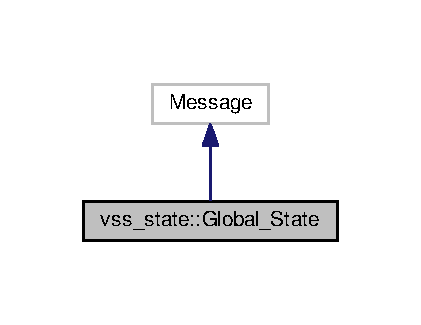
\includegraphics[width=202pt]{classvss__state_1_1Global__State__inherit__graph}
\end{center}
\end{figure}


Collaboration diagram for vss\+\_\+state\+:\+:Global\+\_\+\+State\+:
\nopagebreak
\begin{figure}[H]
\begin{center}
\leavevmode
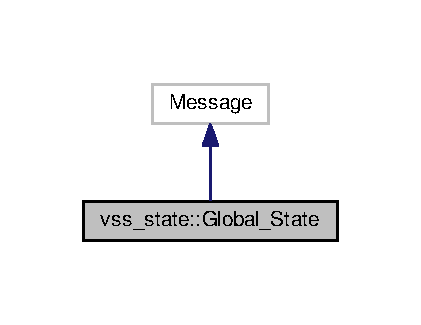
\includegraphics[width=202pt]{classvss__state_1_1Global__State__coll__graph}
\end{center}
\end{figure}
\subsection*{Public Member Functions}
\begin{DoxyCompactItemize}
\item 
{\bfseries Global\+\_\+\+State} (const \hyperlink{classvss__state_1_1Global__State}{Global\+\_\+\+State} \&from)\hypertarget{classvss__state_1_1Global__State_a3a0a70c553656e9c3049308a9513e60c}{}\label{classvss__state_1_1Global__State_a3a0a70c553656e9c3049308a9513e60c}

\item 
\hyperlink{classvss__state_1_1Global__State}{Global\+\_\+\+State} \& {\bfseries operator=} (const \hyperlink{classvss__state_1_1Global__State}{Global\+\_\+\+State} \&from)\hypertarget{classvss__state_1_1Global__State_a01f51f37ae680992a1fd7b0aa3170af9}{}\label{classvss__state_1_1Global__State_a01f51f37ae680992a1fd7b0aa3170af9}

\item 
const \+::google\+::protobuf\+::\+Unknown\+Field\+Set \& {\bfseries unknown\+\_\+fields} () const \hypertarget{classvss__state_1_1Global__State_ad315f5c8ac8db0801d1f554b0f5220e9}{}\label{classvss__state_1_1Global__State_ad315f5c8ac8db0801d1f554b0f5220e9}

\item 
inline\+::google\+::protobuf\+::\+Unknown\+Field\+Set $\ast$ {\bfseries mutable\+\_\+unknown\+\_\+fields} ()\hypertarget{classvss__state_1_1Global__State_a4dbf780222435e650455d532b81dca44}{}\label{classvss__state_1_1Global__State_a4dbf780222435e650455d532b81dca44}

\item 
void {\bfseries Swap} (\hyperlink{classvss__state_1_1Global__State}{Global\+\_\+\+State} $\ast$other)\hypertarget{classvss__state_1_1Global__State_a2b83b57b8673e15692526e3c4ccccc94}{}\label{classvss__state_1_1Global__State_a2b83b57b8673e15692526e3c4ccccc94}

\item 
\hyperlink{classvss__state_1_1Global__State}{Global\+\_\+\+State} $\ast$ {\bfseries New} () const \hypertarget{classvss__state_1_1Global__State_a478df1a0909f344142b866def70f04f1}{}\label{classvss__state_1_1Global__State_a478df1a0909f344142b866def70f04f1}

\item 
void {\bfseries Copy\+From} (const \+::google\+::protobuf\+::\+Message \&from)\hypertarget{classvss__state_1_1Global__State_a5a57651faea985db08eafee9429407d0}{}\label{classvss__state_1_1Global__State_a5a57651faea985db08eafee9429407d0}

\item 
void {\bfseries Merge\+From} (const \+::google\+::protobuf\+::\+Message \&from)\hypertarget{classvss__state_1_1Global__State_ad2905d67a08d3e766963be4d20438dee}{}\label{classvss__state_1_1Global__State_ad2905d67a08d3e766963be4d20438dee}

\item 
void {\bfseries Copy\+From} (const \hyperlink{classvss__state_1_1Global__State}{Global\+\_\+\+State} \&from)\hypertarget{classvss__state_1_1Global__State_aba34386a742582208d2ead2116512710}{}\label{classvss__state_1_1Global__State_aba34386a742582208d2ead2116512710}

\item 
void {\bfseries Merge\+From} (const \hyperlink{classvss__state_1_1Global__State}{Global\+\_\+\+State} \&from)\hypertarget{classvss__state_1_1Global__State_a429e2ccd5b142708a51a3bd069455f52}{}\label{classvss__state_1_1Global__State_a429e2ccd5b142708a51a3bd069455f52}

\item 
void {\bfseries Clear} ()\hypertarget{classvss__state_1_1Global__State_a9c2d7a9cf4dd3c01b53a749e25b0d0fb}{}\label{classvss__state_1_1Global__State_a9c2d7a9cf4dd3c01b53a749e25b0d0fb}

\item 
bool {\bfseries Is\+Initialized} () const \hypertarget{classvss__state_1_1Global__State_ab2c7e2d4af0cd33383e9a4bd1a83113f}{}\label{classvss__state_1_1Global__State_ab2c7e2d4af0cd33383e9a4bd1a83113f}

\item 
int {\bfseries Byte\+Size} () const \hypertarget{classvss__state_1_1Global__State_a10790a0ee8bcc6cff1f704ad0dce113c}{}\label{classvss__state_1_1Global__State_a10790a0ee8bcc6cff1f704ad0dce113c}

\item 
bool {\bfseries Merge\+Partial\+From\+Coded\+Stream} (\+::google\+::protobuf\+::io\+::\+Coded\+Input\+Stream $\ast$input)\hypertarget{classvss__state_1_1Global__State_a6441ee848d925dd1cd3bca5e30c28c7f}{}\label{classvss__state_1_1Global__State_a6441ee848d925dd1cd3bca5e30c28c7f}

\item 
void {\bfseries Serialize\+With\+Cached\+Sizes} (\+::google\+::protobuf\+::io\+::\+Coded\+Output\+Stream $\ast$output) const \hypertarget{classvss__state_1_1Global__State_a01a832c00539c849c8171ff3a228f0df}{}\label{classvss__state_1_1Global__State_a01a832c00539c849c8171ff3a228f0df}

\item 
\+::google\+::protobuf\+::uint8 $\ast$ {\bfseries Serialize\+With\+Cached\+Sizes\+To\+Array} (\+::google\+::protobuf\+::uint8 $\ast$output) const \hypertarget{classvss__state_1_1Global__State_a55efb24ef78b4e7eff557a1c7fd5d7e4}{}\label{classvss__state_1_1Global__State_a55efb24ef78b4e7eff557a1c7fd5d7e4}

\item 
int {\bfseries Get\+Cached\+Size} () const \hypertarget{classvss__state_1_1Global__State_aa94066556db76353540b8b54d77eed2e}{}\label{classvss__state_1_1Global__State_aa94066556db76353540b8b54d77eed2e}

\item 
\+::google\+::protobuf\+::\+Metadata {\bfseries Get\+Metadata} () const \hypertarget{classvss__state_1_1Global__State_a3b2d5b30093df0eb8b20f991dc2d8d9e}{}\label{classvss__state_1_1Global__State_a3b2d5b30093df0eb8b20f991dc2d8d9e}

\item 
bool {\bfseries has\+\_\+id} () const \hypertarget{classvss__state_1_1Global__State_a7d7595f10e8923fada79b67c77ba7cd3}{}\label{classvss__state_1_1Global__State_a7d7595f10e8923fada79b67c77ba7cd3}

\item 
void {\bfseries clear\+\_\+id} ()\hypertarget{classvss__state_1_1Global__State_a0b001773d7aafdb5acef5b36c35f7075}{}\label{classvss__state_1_1Global__State_a0b001773d7aafdb5acef5b36c35f7075}

\item 
inline\+::google\+::protobuf\+::uint32 {\bfseries id} () const \hypertarget{classvss__state_1_1Global__State_ab0ff3c2867cdfda57429a649c9abde17}{}\label{classvss__state_1_1Global__State_ab0ff3c2867cdfda57429a649c9abde17}

\item 
void {\bfseries set\+\_\+id} (\+::google\+::protobuf\+::uint32 value)\hypertarget{classvss__state_1_1Global__State_a183935ca3daee149b526d4a50cce450e}{}\label{classvss__state_1_1Global__State_a183935ca3daee149b526d4a50cce450e}

\item 
bool {\bfseries has\+\_\+origin} () const \hypertarget{classvss__state_1_1Global__State_ab80313b62ce603f182c3e2e1fbea8da5}{}\label{classvss__state_1_1Global__State_ab80313b62ce603f182c3e2e1fbea8da5}

\item 
void {\bfseries clear\+\_\+origin} ()\hypertarget{classvss__state_1_1Global__State_a60aa49b36faa6533ed70bc9e01208282}{}\label{classvss__state_1_1Global__State_a60aa49b36faa6533ed70bc9e01208282}

\item 
bool {\bfseries origin} () const \hypertarget{classvss__state_1_1Global__State_a5b09a31922fe8f976a7e21f2279a1364}{}\label{classvss__state_1_1Global__State_a5b09a31922fe8f976a7e21f2279a1364}

\item 
void {\bfseries set\+\_\+origin} (bool value)\hypertarget{classvss__state_1_1Global__State_ac88223b795690cc57a71f24b315352fc}{}\label{classvss__state_1_1Global__State_ac88223b795690cc57a71f24b315352fc}

\item 
int {\bfseries balls\+\_\+size} () const \hypertarget{classvss__state_1_1Global__State_a5010e0f86563f07ce75ed2138de96ae5}{}\label{classvss__state_1_1Global__State_a5010e0f86563f07ce75ed2138de96ae5}

\item 
void {\bfseries clear\+\_\+balls} ()\hypertarget{classvss__state_1_1Global__State_a738a0947e2c3a450614579e1b7c008e4}{}\label{classvss__state_1_1Global__State_a738a0947e2c3a450614579e1b7c008e4}

\item 
const \+::\hyperlink{classvss__state_1_1Ball__State}{vss\+\_\+state\+::\+Ball\+\_\+\+State} \& {\bfseries balls} (int index) const \hypertarget{classvss__state_1_1Global__State_a6177a6bdab45c96d10c9f64371cd12af}{}\label{classvss__state_1_1Global__State_a6177a6bdab45c96d10c9f64371cd12af}

\item 
inline\+::vss\+\_\+state\+::\+Ball\+\_\+\+State $\ast$ {\bfseries mutable\+\_\+balls} (int index)\hypertarget{classvss__state_1_1Global__State_a88e1c23a1561e6edeaa2c835ad5eb358}{}\label{classvss__state_1_1Global__State_a88e1c23a1561e6edeaa2c835ad5eb358}

\item 
inline\+::vss\+\_\+state\+::\+Ball\+\_\+\+State $\ast$ {\bfseries add\+\_\+balls} ()\hypertarget{classvss__state_1_1Global__State_aa02eca734a92c0f8352fc57dbda91e4e}{}\label{classvss__state_1_1Global__State_aa02eca734a92c0f8352fc57dbda91e4e}

\item 
const \+::google\+::protobuf\+::\+Repeated\+Ptr\+Field$<$ \+::\hyperlink{classvss__state_1_1Ball__State}{vss\+\_\+state\+::\+Ball\+\_\+\+State} $>$ \& {\bfseries balls} () const \hypertarget{classvss__state_1_1Global__State_a792da3990e724f225e585f3e099eab3c}{}\label{classvss__state_1_1Global__State_a792da3990e724f225e585f3e099eab3c}

\item 
inline\+::google\+::protobuf\+::\+Repeated\+Ptr\+Field$<$ \+::\hyperlink{classvss__state_1_1Ball__State}{vss\+\_\+state\+::\+Ball\+\_\+\+State} $>$ $\ast$ {\bfseries mutable\+\_\+balls} ()\hypertarget{classvss__state_1_1Global__State_a47fa3f079e92555b8d86ef916def763e}{}\label{classvss__state_1_1Global__State_a47fa3f079e92555b8d86ef916def763e}

\item 
int {\bfseries robots\+\_\+yellow\+\_\+size} () const \hypertarget{classvss__state_1_1Global__State_ad9605aa1df1cc1a30adc6a88bd85f34f}{}\label{classvss__state_1_1Global__State_ad9605aa1df1cc1a30adc6a88bd85f34f}

\item 
void {\bfseries clear\+\_\+robots\+\_\+yellow} ()\hypertarget{classvss__state_1_1Global__State_a5519565ece84f3f429aa692217fff1f6}{}\label{classvss__state_1_1Global__State_a5519565ece84f3f429aa692217fff1f6}

\item 
const \+::\hyperlink{classvss__state_1_1Robot__State}{vss\+\_\+state\+::\+Robot\+\_\+\+State} \& {\bfseries robots\+\_\+yellow} (int index) const \hypertarget{classvss__state_1_1Global__State_a311a39a8f7be0721ebb684b9bc286ce2}{}\label{classvss__state_1_1Global__State_a311a39a8f7be0721ebb684b9bc286ce2}

\item 
inline\+::vss\+\_\+state\+::\+Robot\+\_\+\+State $\ast$ {\bfseries mutable\+\_\+robots\+\_\+yellow} (int index)\hypertarget{classvss__state_1_1Global__State_a040f90d8bad2e783b1e91077a7c79234}{}\label{classvss__state_1_1Global__State_a040f90d8bad2e783b1e91077a7c79234}

\item 
inline\+::vss\+\_\+state\+::\+Robot\+\_\+\+State $\ast$ {\bfseries add\+\_\+robots\+\_\+yellow} ()\hypertarget{classvss__state_1_1Global__State_aecf340a8be8a26db65bd29ebafcbf1d6}{}\label{classvss__state_1_1Global__State_aecf340a8be8a26db65bd29ebafcbf1d6}

\item 
const \+::google\+::protobuf\+::\+Repeated\+Ptr\+Field$<$ \+::\hyperlink{classvss__state_1_1Robot__State}{vss\+\_\+state\+::\+Robot\+\_\+\+State} $>$ \& {\bfseries robots\+\_\+yellow} () const \hypertarget{classvss__state_1_1Global__State_ad18fe89214728e2c808c8911575ab90b}{}\label{classvss__state_1_1Global__State_ad18fe89214728e2c808c8911575ab90b}

\item 
inline\+::google\+::protobuf\+::\+Repeated\+Ptr\+Field$<$ \+::\hyperlink{classvss__state_1_1Robot__State}{vss\+\_\+state\+::\+Robot\+\_\+\+State} $>$ $\ast$ {\bfseries mutable\+\_\+robots\+\_\+yellow} ()\hypertarget{classvss__state_1_1Global__State_a533514002331b04a673326f334a3e5ce}{}\label{classvss__state_1_1Global__State_a533514002331b04a673326f334a3e5ce}

\item 
int {\bfseries robots\+\_\+blue\+\_\+size} () const \hypertarget{classvss__state_1_1Global__State_ab19e999740e3aa72946a92322bc7f163}{}\label{classvss__state_1_1Global__State_ab19e999740e3aa72946a92322bc7f163}

\item 
void {\bfseries clear\+\_\+robots\+\_\+blue} ()\hypertarget{classvss__state_1_1Global__State_ae88bcfb62ea5ea68673a48aaec873723}{}\label{classvss__state_1_1Global__State_ae88bcfb62ea5ea68673a48aaec873723}

\item 
const \+::\hyperlink{classvss__state_1_1Robot__State}{vss\+\_\+state\+::\+Robot\+\_\+\+State} \& {\bfseries robots\+\_\+blue} (int index) const \hypertarget{classvss__state_1_1Global__State_a92551a5a96b8585f89cc37c55b0c4e46}{}\label{classvss__state_1_1Global__State_a92551a5a96b8585f89cc37c55b0c4e46}

\item 
inline\+::vss\+\_\+state\+::\+Robot\+\_\+\+State $\ast$ {\bfseries mutable\+\_\+robots\+\_\+blue} (int index)\hypertarget{classvss__state_1_1Global__State_a1caf337906ddf4fa47b606dc76cd8a3b}{}\label{classvss__state_1_1Global__State_a1caf337906ddf4fa47b606dc76cd8a3b}

\item 
inline\+::vss\+\_\+state\+::\+Robot\+\_\+\+State $\ast$ {\bfseries add\+\_\+robots\+\_\+blue} ()\hypertarget{classvss__state_1_1Global__State_a3150ca6510afc0a88b10491642dff24a}{}\label{classvss__state_1_1Global__State_a3150ca6510afc0a88b10491642dff24a}

\item 
const \+::google\+::protobuf\+::\+Repeated\+Ptr\+Field$<$ \+::\hyperlink{classvss__state_1_1Robot__State}{vss\+\_\+state\+::\+Robot\+\_\+\+State} $>$ \& {\bfseries robots\+\_\+blue} () const \hypertarget{classvss__state_1_1Global__State_ad659e30adf37a0e412765337eb28f233}{}\label{classvss__state_1_1Global__State_ad659e30adf37a0e412765337eb28f233}

\item 
inline\+::google\+::protobuf\+::\+Repeated\+Ptr\+Field$<$ \+::\hyperlink{classvss__state_1_1Robot__State}{vss\+\_\+state\+::\+Robot\+\_\+\+State} $>$ $\ast$ {\bfseries mutable\+\_\+robots\+\_\+blue} ()\hypertarget{classvss__state_1_1Global__State_a73be200ff11edfc042221b579672d3b4}{}\label{classvss__state_1_1Global__State_a73be200ff11edfc042221b579672d3b4}

\end{DoxyCompactItemize}
\subsection*{Static Public Member Functions}
\begin{DoxyCompactItemize}
\item 
static const \+::google\+::protobuf\+::\+Descriptor $\ast$ {\bfseries descriptor} ()\hypertarget{classvss__state_1_1Global__State_af5963eb38d472f2508e180fdf42c4a22}{}\label{classvss__state_1_1Global__State_af5963eb38d472f2508e180fdf42c4a22}

\item 
static const \hyperlink{classvss__state_1_1Global__State}{Global\+\_\+\+State} \& {\bfseries default\+\_\+instance} ()\hypertarget{classvss__state_1_1Global__State_a1bf08b600180f360bcd37c58f3e50b16}{}\label{classvss__state_1_1Global__State_a1bf08b600180f360bcd37c58f3e50b16}

\end{DoxyCompactItemize}
\subsection*{Static Public Attributes}
\begin{DoxyCompactItemize}
\item 
static const int {\bfseries k\+Id\+Field\+Number} = 1\hypertarget{classvss__state_1_1Global__State_adc3acf2d9111dd7e0e442b1c8f8743ab}{}\label{classvss__state_1_1Global__State_adc3acf2d9111dd7e0e442b1c8f8743ab}

\item 
static const int {\bfseries k\+Origin\+Field\+Number} = 2\hypertarget{classvss__state_1_1Global__State_a124e80222f404a8607d383c6b626b98a}{}\label{classvss__state_1_1Global__State_a124e80222f404a8607d383c6b626b98a}

\item 
static const int {\bfseries k\+Balls\+Field\+Number} = 3\hypertarget{classvss__state_1_1Global__State_a7ccc5ad24ae6460151ee94fd5f3800f5}{}\label{classvss__state_1_1Global__State_a7ccc5ad24ae6460151ee94fd5f3800f5}

\item 
static const int {\bfseries k\+Robots\+Yellow\+Field\+Number} = 4\hypertarget{classvss__state_1_1Global__State_a3dbd17117a81ad417c69ca945668edaa}{}\label{classvss__state_1_1Global__State_a3dbd17117a81ad417c69ca945668edaa}

\item 
static const int {\bfseries k\+Robots\+Blue\+Field\+Number} = 5\hypertarget{classvss__state_1_1Global__State_a69fd6df3aa2671364cb92838e3824e81}{}\label{classvss__state_1_1Global__State_a69fd6df3aa2671364cb92838e3824e81}

\end{DoxyCompactItemize}
\subsection*{Friends}
\begin{DoxyCompactItemize}
\item 
void {\bfseries protobuf\+\_\+\+Add\+Desc\+\_\+state\+\_\+2eproto} ()\hypertarget{classvss__state_1_1Global__State_aab1a2c258f8122a403a979ff57e2a706}{}\label{classvss__state_1_1Global__State_aab1a2c258f8122a403a979ff57e2a706}

\item 
void {\bfseries protobuf\+\_\+\+Assign\+Desc\+\_\+state\+\_\+2eproto} ()\hypertarget{classvss__state_1_1Global__State_a57d9367bc8a7a94ead11d11194cca1b6}{}\label{classvss__state_1_1Global__State_a57d9367bc8a7a94ead11d11194cca1b6}

\item 
void {\bfseries protobuf\+\_\+\+Shutdown\+File\+\_\+state\+\_\+2eproto} ()\hypertarget{classvss__state_1_1Global__State_a4e6dc5e8e72799859c4e9556d090e57d}{}\label{classvss__state_1_1Global__State_a4e6dc5e8e72799859c4e9556d090e57d}

\end{DoxyCompactItemize}


The documentation for this class was generated from the following files\+:\begin{DoxyCompactItemize}
\item 
/home/johnathan/\+Repositories/\+S\+I\+R\+Lab/\+V\+S\+S-\/\+Vision/src/protos/state.\+pb.\+h\item 
/home/johnathan/\+Repositories/\+S\+I\+R\+Lab/\+V\+S\+S-\/\+Vision/src/protos/state.\+pb.\+cc\end{DoxyCompactItemize}

\hypertarget{classInterface}{}\section{Interface Class Reference}
\label{classInterface}\index{Interface@{Interface}}


This class is responsible for handle the communicatio between V\+S\+S-\/\+Vision, V\+S\+S-\/\+Simulator, V\+S\+S-\/\+Viewer and V\+S\+S-\/\+Sample\+Stratey.  




{\ttfamily \#include $<$interface.\+h$>$}



Collaboration diagram for Interface\+:
\nopagebreak
\begin{figure}[H]
\begin{center}
\leavevmode
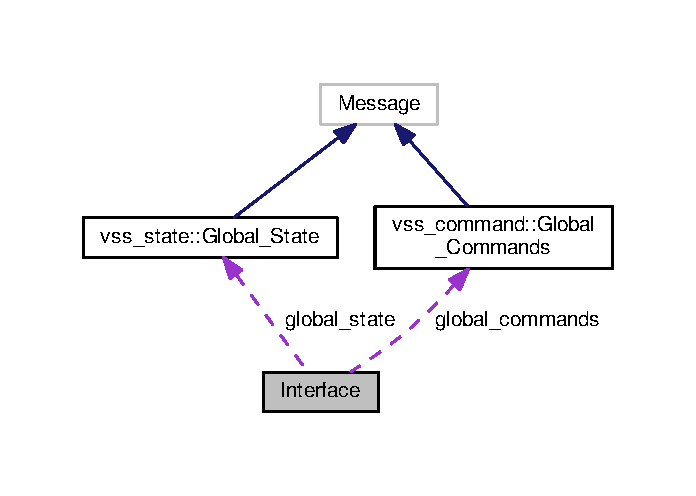
\includegraphics[width=334pt]{classInterface__coll__graph}
\end{center}
\end{figure}
\subsection*{Public Member Functions}
\begin{DoxyCompactItemize}
\item 
void {\bfseries create\+Socket\+Send\+State} (\hyperlink{classvss__state_1_1Global__State}{vss\+\_\+state\+::\+Global\+\_\+\+State} $\ast$)\hypertarget{classInterface_a76752c5d305865777405fd8f36e4b9fd}{}\label{classInterface_a76752c5d305865777405fd8f36e4b9fd}

\item 
void {\bfseries send\+State} ()\hypertarget{classInterface_a9de875408d6ec60ef952d167ab244819}{}\label{classInterface_a9de875408d6ec60ef952d167ab244819}

\item 
void {\bfseries create\+Socket\+Receive\+State} (\hyperlink{classvss__state_1_1Global__State}{vss\+\_\+state\+::\+Global\+\_\+\+State} $\ast$)\hypertarget{classInterface_ad7466b43bc53a4cd5225c280cf81b2cc}{}\label{classInterface_ad7466b43bc53a4cd5225c280cf81b2cc}

\item 
void {\bfseries receive\+State} ()\hypertarget{classInterface_abba50a9d10639aa5b2f4a45be31b4062}{}\label{classInterface_abba50a9d10639aa5b2f4a45be31b4062}

\item 
void {\bfseries create\+Loop\+Send\+Commands\+Team1} (\hyperlink{classvss__command_1_1Global__Commands}{vss\+\_\+command\+::\+Global\+\_\+\+Commands} $\ast$)\hypertarget{classInterface_a856aa7ba2462cb787bff454998ac03fa}{}\label{classInterface_a856aa7ba2462cb787bff454998ac03fa}

\item 
void {\bfseries create\+Loop\+Receive\+Commands\+Team1} (\hyperlink{classvss__command_1_1Global__Commands}{vss\+\_\+command\+::\+Global\+\_\+\+Commands} $\ast$)\hypertarget{classInterface_a9421fb07f3190cff0ab4198587de4b87}{}\label{classInterface_a9421fb07f3190cff0ab4198587de4b87}

\item 
void {\bfseries create\+Loop\+Send\+Commands\+Team2} (\hyperlink{classvss__command_1_1Global__Commands}{vss\+\_\+command\+::\+Global\+\_\+\+Commands} $\ast$)\hypertarget{classInterface_a59f5b2b5043433cbd42729baf84533e1}{}\label{classInterface_a59f5b2b5043433cbd42729baf84533e1}

\item 
void {\bfseries create\+Loop\+Receive\+Commands\+Team2} (\hyperlink{classvss__command_1_1Global__Commands}{vss\+\_\+command\+::\+Global\+\_\+\+Commands} $\ast$)\hypertarget{classInterface_aff3b574fe1147f93011c1deef6ec5505}{}\label{classInterface_aff3b574fe1147f93011c1deef6ec5505}

\item 
void {\bfseries print\+State} ()\hypertarget{classInterface_ab8f9122465d78b9e41bfde9ea560a657}{}\label{classInterface_ab8f9122465d78b9e41bfde9ea560a657}

\item 
void {\bfseries print\+Command} ()\hypertarget{classInterface_aaa4e713b2b72649d5253c83bf9e2416a}{}\label{classInterface_aaa4e713b2b72649d5253c83bf9e2416a}

\end{DoxyCompactItemize}
\subsection*{Protected Attributes}
\begin{DoxyCompactItemize}
\item 
zmq\+::message\+\_\+t {\bfseries request}\hypertarget{classInterface_a99822a3bea1a0cb8c72670db0f797689}{}\label{classInterface_a99822a3bea1a0cb8c72670db0f797689}

\item 
zmq\+::context\+\_\+t $\ast$ {\bfseries context}\hypertarget{classInterface_a7a2bda6046550893e9454930636e76d5}{}\label{classInterface_a7a2bda6046550893e9454930636e76d5}

\item 
zmq\+::socket\+\_\+t $\ast$ {\bfseries socket}\hypertarget{classInterface_af38139f534f08df8b3dc9f29001e9584}{}\label{classInterface_af38139f534f08df8b3dc9f29001e9584}

\item 
\hyperlink{classvss__state_1_1Global__State}{vss\+\_\+state\+::\+Global\+\_\+\+State} $\ast$ {\bfseries global\+\_\+state}\hypertarget{classInterface_ac488bcc6708103cb36d132c895efa7a0}{}\label{classInterface_ac488bcc6708103cb36d132c895efa7a0}

\item 
\hyperlink{classvss__command_1_1Global__Commands}{vss\+\_\+command\+::\+Global\+\_\+\+Commands} $\ast$ {\bfseries global\+\_\+commands}\hypertarget{classInterface_a0109a54da68b3e7cd0c652f6cdd75abe}{}\label{classInterface_a0109a54da68b3e7cd0c652f6cdd75abe}

\item 
const char $\ast$ {\bfseries addr\+\_\+server\+\_\+multicast} = \char`\"{}tcp\+://$\ast$\+:5555\char`\"{}\hypertarget{classInterface_a13af5d0710e73dc30603c7fd13e763c9}{}\label{classInterface_a13af5d0710e73dc30603c7fd13e763c9}

\item 
const char $\ast$ {\bfseries addr\+\_\+client\+\_\+multicast} = \char`\"{}tcp\+://localhost\+:5555\char`\"{}\hypertarget{classInterface_a8215c1845687c3bceb55d2ab21f7f1ff}{}\label{classInterface_a8215c1845687c3bceb55d2ab21f7f1ff}

\item 
const char $\ast$ {\bfseries addr\+\_\+server\+\_\+simulator\+\_\+team1} = \char`\"{}tcp\+://$\ast$\+:5556\char`\"{}\hypertarget{classInterface_a4315a24cd5d7156ccb6da180cc5a825e}{}\label{classInterface_a4315a24cd5d7156ccb6da180cc5a825e}

\item 
const char $\ast$ {\bfseries addr\+\_\+client\+\_\+simulator\+\_\+team1} = \char`\"{}tcp\+://localhost\+:5556\char`\"{}\hypertarget{classInterface_aa05d667c54fc41c5dc6fe7aa8a85ef5d}{}\label{classInterface_aa05d667c54fc41c5dc6fe7aa8a85ef5d}

\item 
const char $\ast$ {\bfseries addr\+\_\+server\+\_\+simulator\+\_\+team2} = \char`\"{}tcp\+://$\ast$\+:5557\char`\"{}\hypertarget{classInterface_ae358e6d8cb691934a5dc23c4a718082b}{}\label{classInterface_ae358e6d8cb691934a5dc23c4a718082b}

\item 
const char $\ast$ {\bfseries addr\+\_\+client\+\_\+simulator\+\_\+team2} = \char`\"{}tcp\+://localhost\+:5557\char`\"{}\hypertarget{classInterface_adad17a36b3382235441861a3648bd807}{}\label{classInterface_adad17a36b3382235441861a3648bd807}

\end{DoxyCompactItemize}


\subsection{Detailed Description}
This class is responsible for handle the communicatio between V\+S\+S-\/\+Vision, V\+S\+S-\/\+Simulator, V\+S\+S-\/\+Viewer and V\+S\+S-\/\+Sample\+Stratey. 

The documentation for this class was generated from the following files\+:\begin{DoxyCompactItemize}
\item 
/home/johnathan/\+Repositories/\+S\+I\+R\+Lab/\+V\+S\+S-\/\+Vision/src/interface.\+h\item 
/home/johnathan/\+Repositories/\+S\+I\+R\+Lab/\+V\+S\+S-\/\+Vision/src/interface.\+cpp\end{DoxyCompactItemize}

\hypertarget{classMainWindow}{}\section{Main\+Window Class Reference}
\label{classMainWindow}\index{Main\+Window@{Main\+Window}}


This class is the main window of the software.  




{\ttfamily \#include $<$mainwindow.\+h$>$}



Inheritance diagram for Main\+Window\+:
\nopagebreak
\begin{figure}[H]
\begin{center}
\leavevmode
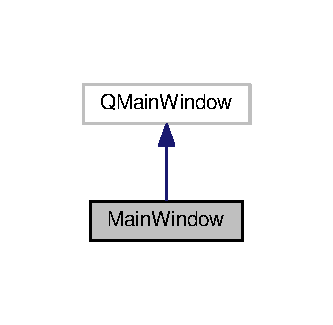
\includegraphics[width=160pt]{classMainWindow__inherit__graph}
\end{center}
\end{figure}


Collaboration diagram for Main\+Window\+:
\nopagebreak
\begin{figure}[H]
\begin{center}
\leavevmode
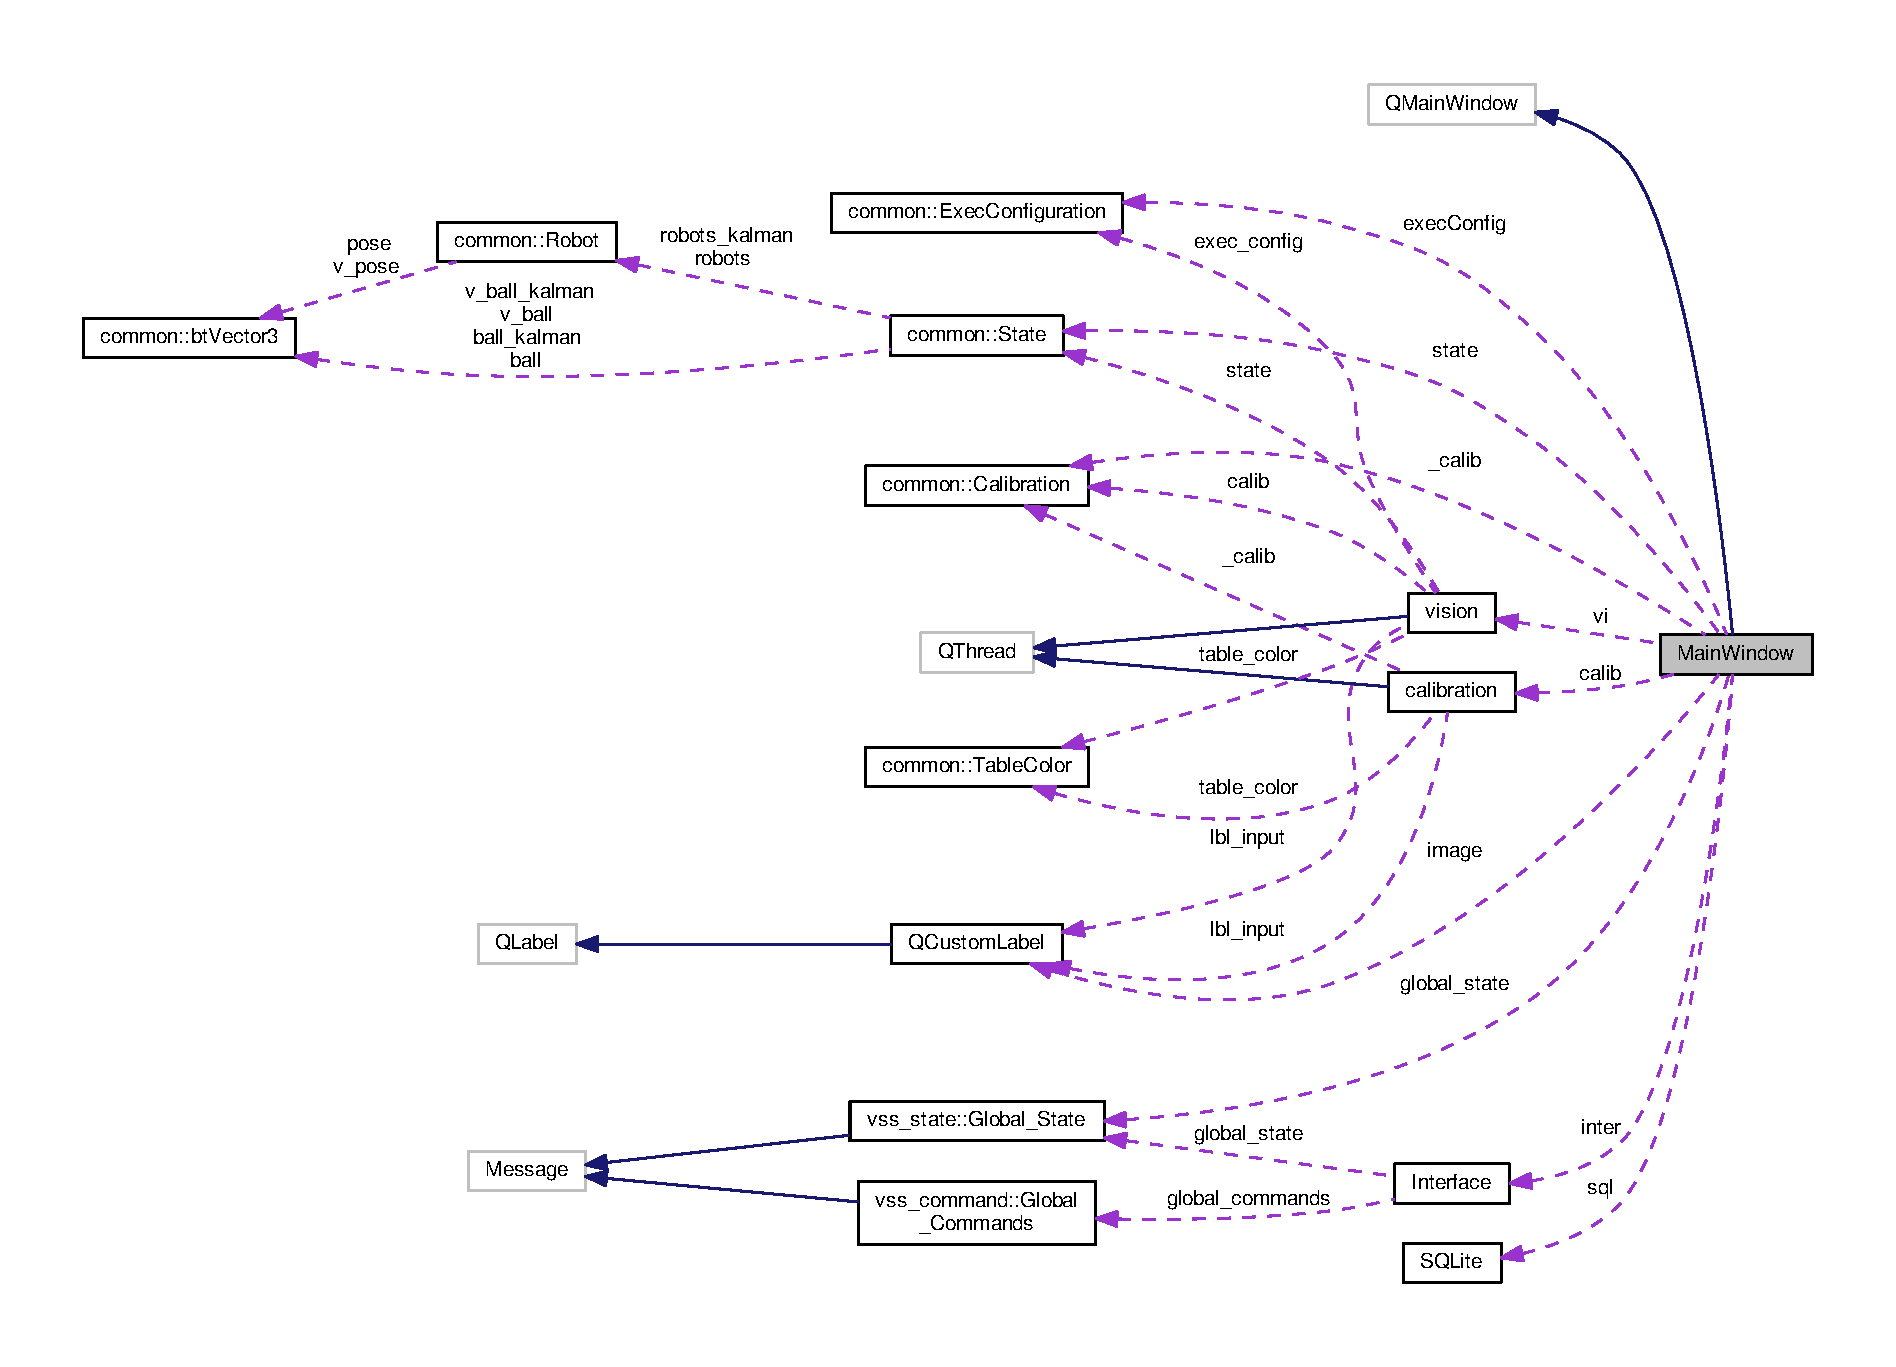
\includegraphics[width=350pt]{classMainWindow__coll__graph}
\end{center}
\end{figure}
\subsection*{Public Slots}
\begin{DoxyCompactItemize}
\item 
void \hyperlink{classMainWindow_a8501942bff62e974d8b4565257538c0f}{mouse\+Current\+Pos} ()
\begin{DoxyCompactList}\small\item\em Method that get the signal from move the mouse inside \hyperlink{classQCustomLabel}{Q\+Custom\+Label} input image. \end{DoxyCompactList}\item 
void \hyperlink{classMainWindow_a638cd98f8b593e868829541f2b9f6b63}{mouse\+Left\+Pressed} ()
\begin{DoxyCompactList}\small\item\em Method that get the signal from left click inside \hyperlink{classQCustomLabel}{Q\+Custom\+Label} input image. \end{DoxyCompactList}\item 
void \hyperlink{classMainWindow_ab78b5ef982f3e4d7613a03a9da6fb987}{mouse\+Right\+Pressed} ()
\begin{DoxyCompactList}\small\item\em Method that get the signal from right click inside \hyperlink{classQCustomLabel}{Q\+Custom\+Label} input image. \end{DoxyCompactList}\item 
void \hyperlink{classMainWindow_a089e5ff94a64d40dabe0a6eb36cc08f8}{mouse\+Released} ()\hypertarget{classMainWindow_a089e5ff94a64d40dabe0a6eb36cc08f8}{}\label{classMainWindow_a089e5ff94a64d40dabe0a6eb36cc08f8}

\begin{DoxyCompactList}\small\item\em Method that get the signal from release left click inside \hyperlink{classQCustomLabel}{Q\+Custom\+Label} input image. \end{DoxyCompactList}\item 
void \hyperlink{classMainWindow_a0b3abf28e1dab2b5321f1e53adb8b8c4}{mouse\+Leave} ()\hypertarget{classMainWindow_a0b3abf28e1dab2b5321f1e53adb8b8c4}{}\label{classMainWindow_a0b3abf28e1dab2b5321f1e53adb8b8c4}

\begin{DoxyCompactList}\small\item\em Method that get the signal from release the mouse from \hyperlink{classQCustomLabel}{Q\+Custom\+Label} input image. \end{DoxyCompactList}\item 
void \hyperlink{classMainWindow_a3f53a2549c74484b5d67d79914778c35}{evt\+Calibration\+Colors} ()
\begin{DoxyCompactList}\small\item\em Method that get the signal from click on Q\+Push\+Button Do Calibration Colors. \end{DoxyCompactList}\item 
void \hyperlink{classMainWindow_a202a597ababe8aa1fd3c821e703599b6}{evt\+Vision} ()
\begin{DoxyCompactList}\small\item\em Method that get the signal from click on Q\+Push\+Button Run Vision. \end{DoxyCompactList}\item 
void \hyperlink{classMainWindow_a774d98597bb682ed113f07a7068f6496}{evt\+Calibration\+Cam} ()
\begin{DoxyCompactList}\small\item\em Method that get the signal from click on Q\+Push\+Button Do Calibration Camera. \end{DoxyCompactList}\item 
void \hyperlink{classMainWindow_afb1276b4a282f8678e25b0ec1a0195c9}{checkbox\+Camera} (int)
\begin{DoxyCompactList}\small\item\em Method that get the signal from click on Q\+Checkbox of use camera. \end{DoxyCompactList}\item 
void \hyperlink{classMainWindow_aa0266c5762b37479a888fba709aefbee}{checkbox\+Image} (int)
\begin{DoxyCompactList}\small\item\em Method that get the signal from click on Q\+Checkbox of use image. \end{DoxyCompactList}\item 
void \hyperlink{classMainWindow_a33f858356490a2440246af76ca922392}{checkbox\+Video} (int)
\begin{DoxyCompactList}\small\item\em Method that get the signal from click on Q\+Checkbox of use video. \end{DoxyCompactList}\item 
void \hyperlink{classMainWindow_afffdad16c118e2351cec7b47c243e9b1}{update\+Hmin} (int)\hypertarget{classMainWindow_afffdad16c118e2351cec7b47c243e9b1}{}\label{classMainWindow_afffdad16c118e2351cec7b47c243e9b1}

\begin{DoxyCompactList}\small\item\em Method that get the signal from slide on H\+S\+V-\/\+Hmin. \end{DoxyCompactList}\item 
void \hyperlink{classMainWindow_a11f3aa0b929685232b671cd378d31972}{update\+Smin} (int)\hypertarget{classMainWindow_a11f3aa0b929685232b671cd378d31972}{}\label{classMainWindow_a11f3aa0b929685232b671cd378d31972}

\begin{DoxyCompactList}\small\item\em Method that get the signal from slide on H\+S\+V-\/\+S\+Min. \end{DoxyCompactList}\item 
void \hyperlink{classMainWindow_a43da847294670cdaaa17f2235888b47a}{update\+Vmin} (int)\hypertarget{classMainWindow_a43da847294670cdaaa17f2235888b47a}{}\label{classMainWindow_a43da847294670cdaaa17f2235888b47a}

\begin{DoxyCompactList}\small\item\em Method that get the signal from slide on H\+S\+V-\/\+Vmin. \end{DoxyCompactList}\item 
void \hyperlink{classMainWindow_af3d7639f0c28d053fdc10484b109ac99}{update\+Hmax} (int)\hypertarget{classMainWindow_af3d7639f0c28d053fdc10484b109ac99}{}\label{classMainWindow_af3d7639f0c28d053fdc10484b109ac99}

\begin{DoxyCompactList}\small\item\em Method that get the signal from slide on H\+S\+V-\/\+Hmax. \end{DoxyCompactList}\item 
void \hyperlink{classMainWindow_a2c08d2f7c55d78c30b12dd3a16905d7b}{update\+Smax} (int)\hypertarget{classMainWindow_a2c08d2f7c55d78c30b12dd3a16905d7b}{}\label{classMainWindow_a2c08d2f7c55d78c30b12dd3a16905d7b}

\begin{DoxyCompactList}\small\item\em Method that get the signal from slide on H\+S\+V-\/\+Smax. \end{DoxyCompactList}\item 
void \hyperlink{classMainWindow_a2f06abb52f3906ae6177f7fc9f859505}{update\+Vmax} (int)\hypertarget{classMainWindow_a2f06abb52f3906ae6177f7fc9f859505}{}\label{classMainWindow_a2f06abb52f3906ae6177f7fc9f859505}

\begin{DoxyCompactList}\small\item\em Method that get the signal from slide on H\+S\+V-\/\+Vmax. \end{DoxyCompactList}\item 
void \hyperlink{classMainWindow_a6c6ff08babc2f86d2484aa7a97b671e0}{update\+Rotation} (int)\hypertarget{classMainWindow_a6c6ff08babc2f86d2484aa7a97b671e0}{}\label{classMainWindow_a6c6ff08babc2f86d2484aa7a97b671e0}

\begin{DoxyCompactList}\small\item\em Method that get the signal from slide on Rotation. \end{DoxyCompactList}\item 
void \hyperlink{classMainWindow_a05ab58ddf53a08fd87eaa649a613a7de}{get\+New\+Image\+Calib} ()\hypertarget{classMainWindow_a05ab58ddf53a08fd87eaa649a613a7de}{}\label{classMainWindow_a05ab58ddf53a08fd87eaa649a613a7de}

\begin{DoxyCompactList}\small\item\em Method that get the signal has\+\_\+new\+\_\+image() from calibration. \end{DoxyCompactList}\item 
void \hyperlink{classMainWindow_aa319f5224d5e0532849393c96e85f006}{get\+New\+State\+Vision} ()\hypertarget{classMainWindow_aa319f5224d5e0532849393c96e85f006}{}\label{classMainWindow_aa319f5224d5e0532849393c96e85f006}

\begin{DoxyCompactList}\small\item\em Method that get the signal has\+\_\+new\+\_\+state() from vision. \end{DoxyCompactList}\end{DoxyCompactItemize}
\subsection*{Public Member Functions}
\begin{DoxyCompactItemize}
\item 
\hyperlink{classMainWindow_a8b244be8b7b7db1b08de2a2acb9409db}{Main\+Window} (Q\+Widget $\ast$parent=0)
\end{DoxyCompactItemize}
\subsection*{Protected Member Functions}
\begin{DoxyCompactItemize}
\item 
void \hyperlink{classMainWindow_a904aeccdff7a61af31954793944ef364}{build\+Trees} ()
\begin{DoxyCompactList}\small\item\em Method responsible for build all the left tab. \end{DoxyCompactList}\item 
void \hyperlink{classMainWindow_a7f3e055a4f80071b7265cc32d10b1a29}{add\+Main\+Item} ()
\begin{DoxyCompactList}\small\item\em Method responsible for add the main item \char`\"{}\+Yellow box\char`\"{}. \end{DoxyCompactList}\item 
void \hyperlink{classMainWindow_aa2cc5fc73f649129465c371368185189}{add\+Input\+Data\+Item} ()\hypertarget{classMainWindow_aa2cc5fc73f649129465c371368185189}{}\label{classMainWindow_aa2cc5fc73f649129465c371368185189}

\begin{DoxyCompactList}\small\item\em Method responsible for add the item of choose input data. \end{DoxyCompactList}\item 
void \hyperlink{classMainWindow_ae887769c9a6614f6827afdb74ab9cd12}{add\+Camera\+Calibration\+Item} ()\hypertarget{classMainWindow_ae887769c9a6614f6827afdb74ab9cd12}{}\label{classMainWindow_ae887769c9a6614f6827afdb74ab9cd12}

\begin{DoxyCompactList}\small\item\em Method reponsible for add the item of calibrate camera, cut points and rotation. \end{DoxyCompactList}\item 
void \hyperlink{classMainWindow_a659cf521c8e7053eaba4971293050883}{add\+Blob\+Finding\+Item} ()\hypertarget{classMainWindow_a659cf521c8e7053eaba4971293050883}{}\label{classMainWindow_a659cf521c8e7053eaba4971293050883}

\begin{DoxyCompactList}\small\item\em Method responsible for add the item of set parameters of vision, like for blobs\+: area-\/min, area-\/max, proportion-\/max, proportion-\/min. \end{DoxyCompactList}\item 
void \hyperlink{classMainWindow_aa30ad88d5b5acbf1cc9f70840d416e24}{add\+Visualization\+Item} ()\hypertarget{classMainWindow_aa30ad88d5b5acbf1cc9f70840d416e24}{}\label{classMainWindow_aa30ad88d5b5acbf1cc9f70840d416e24}

\begin{DoxyCompactList}\small\item\em Method responsible for add the item of set visualization (D\+E\+P\+R\+E\+C\+A\+T\+ED) \end{DoxyCompactList}\item 
void \hyperlink{classMainWindow_a9f08218f96f231b1615ce24d933b15ce}{add\+Define\+Patterns\+Item} ()\hypertarget{classMainWindow_a9f08218f96f231b1615ce24d933b15ce}{}\label{classMainWindow_a9f08218f96f231b1615ce24d933b15ce}

\begin{DoxyCompactList}\small\item\em Method responsible for add the item that defines the type of pattern of colors (T\+O\+DO) \end{DoxyCompactList}\item 
void \hyperlink{classMainWindow_a4d645b048c765c34481cb4e7749af6cf}{add\+Execution\+Config} ()\hypertarget{classMainWindow_a4d645b048c765c34481cb4e7749af6cf}{}\label{classMainWindow_a4d645b048c765c34481cb4e7749af6cf}

\begin{DoxyCompactList}\small\item\em Method responsible for add the item of define the configuration of colors of each team. \end{DoxyCompactList}\item 
void \hyperlink{classMainWindow_a5fa2d31a87dcc532276b17ab49712add}{add\+Calibrate\+Colors} ()\hypertarget{classMainWindow_a5fa2d31a87dcc532276b17ab49712add}{}\label{classMainWindow_a5fa2d31a87dcc532276b17ab49712add}

\begin{DoxyCompactList}\small\item\em Method responsible for add the item of calibration of colors. \end{DoxyCompactList}\item 
void {\bfseries add\+Vision\+Options} ()\hypertarget{classMainWindow_a84f4504e9262385ede0b0e89832181f9}{}\label{classMainWindow_a84f4504e9262385ede0b0e89832181f9}

\item 
void \hyperlink{classMainWindow_ad4406d1714477f132de211c3351365cb}{add\+Net\+Options} ()\hypertarget{classMainWindow_ad4406d1714477f132de211c3351365cb}{}\label{classMainWindow_ad4406d1714477f132de211c3351365cb}

\begin{DoxyCompactList}\small\item\em Method responsible for add the item of define IP and P\+O\+RT for interface. \end{DoxyCompactList}\item 
void \hyperlink{classMainWindow_adb0b4159e334fb5b388a9eb1c4b8f5ca}{add\+Execution\+Options} ()\hypertarget{classMainWindow_adb0b4159e334fb5b388a9eb1c4b8f5ca}{}\label{classMainWindow_adb0b4159e334fb5b388a9eb1c4b8f5ca}

\begin{DoxyCompactList}\small\item\em Method reponsible form add the item of initializes the vision tracking. \end{DoxyCompactList}\item 
void \hyperlink{classMainWindow_ab514a3e2e2feb11fe562bb5f5687c260}{init\+Calibration\+Colors} ()\hypertarget{classMainWindow_ab514a3e2e2feb11fe562bb5f5687c260}{}\label{classMainWindow_ab514a3e2e2feb11fe562bb5f5687c260}

\begin{DoxyCompactList}\small\item\em Method responsible for update the layout for turn on the calibration. \end{DoxyCompactList}\item 
void \hyperlink{classMainWindow_aaed408509f0ec209d5113b6d838f223a}{finish\+Calibration\+Colors} ()\hypertarget{classMainWindow_aaed408509f0ec209d5113b6d838f223a}{}\label{classMainWindow_aaed408509f0ec209d5113b6d838f223a}

\begin{DoxyCompactList}\small\item\em Method responsible for update the layout for turn off the calibration. \end{DoxyCompactList}\item 
void {\bfseries init\+Calibration\+Camera} ()\hypertarget{classMainWindow_afcee03b23b74fc2730a43c282130ed3f}{}\label{classMainWindow_afcee03b23b74fc2730a43c282130ed3f}

\item 
void {\bfseries finish\+Calibration\+Camera} ()\hypertarget{classMainWindow_a535252d6997fbf9460ab40a072900a56}{}\label{classMainWindow_a535252d6997fbf9460ab40a072900a56}

\item 
void \hyperlink{classMainWindow_afe574227eabad29af617957c1c74f11f}{init\+Plot\+Values} ()\hypertarget{classMainWindow_afe574227eabad29af617957c1c74f11f}{}\label{classMainWindow_afe574227eabad29af617957c1c74f11f}

\begin{DoxyCompactList}\small\item\em Method responsible for update the layout for turn on the vision. \end{DoxyCompactList}\item 
void \hyperlink{classMainWindow_a71bb19c8988c81c52cf8856295584ff5}{finish\+Plot\+Values} ()\hypertarget{classMainWindow_a71bb19c8988c81c52cf8856295584ff5}{}\label{classMainWindow_a71bb19c8988c81c52cf8856295584ff5}

\begin{DoxyCompactList}\small\item\em Method responsible for update the layout for turn off the vision. \end{DoxyCompactList}\item 
void \hyperlink{classMainWindow_aee8cb88ae764bcfb12963ab2a1fa9e65}{update\+Values\+H\+SV} ()\hypertarget{classMainWindow_aee8cb88ae764bcfb12963ab2a1fa9e65}{}\label{classMainWindow_aee8cb88ae764bcfb12963ab2a1fa9e65}

\begin{DoxyCompactList}\small\item\em Method responsible for update de commom\+::\+Vision\+Color of calibration, depends of id\+\_\+color in \hyperlink{structcommon_1_1TableColor}{common\+::\+Table\+Color}. \end{DoxyCompactList}\item 
void \hyperlink{classMainWindow_a6a418df110068fb09bd60ce785c05926}{update\+\_\+hsv\+\_\+s} ()\hypertarget{classMainWindow_a6a418df110068fb09bd60ce785c05926}{}\label{classMainWindow_a6a418df110068fb09bd60ce785c05926}

\begin{DoxyCompactList}\small\item\em Method responsible for update the slide H\+S\+V-\/\+Smin and H\+S\+V-\/\+Smax, with the id\+\_\+color in \hyperlink{structcommon_1_1TableColor}{common\+::\+Table\+Color}. \end{DoxyCompactList}\item 
void \hyperlink{classMainWindow_a0ec10b5c5cd98c5aa086bf91793c9d7e}{get\+All\+Devices} ()
\begin{DoxyCompactList}\small\item\em Method responsible for get all cameras on PC. \end{DoxyCompactList}\item 
void \hyperlink{classMainWindow_a62c1577587f33bc89c823d3ea3f23bda}{define\+Colors} ()\hypertarget{classMainWindow_a62c1577587f33bc89c823d3ea3f23bda}{}\label{classMainWindow_a62c1577587f33bc89c823d3ea3f23bda}

\begin{DoxyCompactList}\small\item\em Method responsible for define the colors that gonna be used on vision. \end{DoxyCompactList}\item 
int \hyperlink{classMainWindow_a7d8385cfb0a4a1bbb38ac943010962d9}{translate\+Color} (Q\+String)\hypertarget{classMainWindow_a7d8385cfb0a4a1bbb38ac943010962d9}{}\label{classMainWindow_a7d8385cfb0a4a1bbb38ac943010962d9}

\begin{DoxyCompactList}\small\item\em Method responsible for translate the colors on Q\+Checkbox to vector. \end{DoxyCompactList}\end{DoxyCompactItemize}
\subsection*{Protected Attributes}
\begin{DoxyCompactItemize}
\item 
\hyperlink{classInterface}{Interface} {\bfseries inter}\hypertarget{classMainWindow_ad242666fbf3bdf53bae55cbc178a7b05}{}\label{classMainWindow_ad242666fbf3bdf53bae55cbc178a7b05}

\item 
\hyperlink{classcalibration}{calibration} $\ast$ {\bfseries calib}\hypertarget{classMainWindow_ae41ab8a2caab2b5b1a1432ce15eb0e51}{}\label{classMainWindow_ae41ab8a2caab2b5b1a1432ce15eb0e51}

\item 
\hyperlink{classvision}{vision} $\ast$ {\bfseries vi}\hypertarget{classMainWindow_aed5906811bbf1191aa952deb4279e36f}{}\label{classMainWindow_aed5906811bbf1191aa952deb4279e36f}

\item 
\hyperlink{classSQLite}{S\+Q\+Lite} $\ast$ {\bfseries sql}\hypertarget{classMainWindow_a27a47dcf3589dd010ce7803cb3b2ff85}{}\label{classMainWindow_a27a47dcf3589dd010ce7803cb3b2ff85}

\item 
Ui\+::\+Main\+Window $\ast$ {\bfseries ui}\hypertarget{classMainWindow_a35466a70ed47252a0191168126a352a5}{}\label{classMainWindow_a35466a70ed47252a0191168126a352a5}

\item 
\hyperlink{classvss__state_1_1Global__State}{vss\+\_\+state\+::\+Global\+\_\+\+State} $\ast$ {\bfseries global\+\_\+state}\hypertarget{classMainWindow_a6b6de60876dfab34a424a2603a5edb82}{}\label{classMainWindow_a6b6de60876dfab34a424a2603a5edb82}

\item 
Q\+Icon {\bfseries blockdevice}\hypertarget{classMainWindow_add3756176df4e7230246c550d9b6e2db}{}\label{classMainWindow_add3756176df4e7230246c550d9b6e2db}

\item 
Q\+Icon {\bfseries ksame}\hypertarget{classMainWindow_ac1beb6db1d37a2a6c3d66688aefd9a66}{}\label{classMainWindow_ac1beb6db1d37a2a6c3d66688aefd9a66}

\item 
Q\+Icon {\bfseries kdf}\hypertarget{classMainWindow_a9d4567d65912ab7578d00827129c4755}{}\label{classMainWindow_a9d4567d65912ab7578d00827129c4755}

\item 
Q\+Icon {\bfseries package}\hypertarget{classMainWindow_a211b3162d03a5c229ac006150286429e}{}\label{classMainWindow_a211b3162d03a5c229ac006150286429e}

\item 
Q\+Tree\+Widget\+Item $\ast$ {\bfseries main\+Item}\hypertarget{classMainWindow_a4a0290f0cbe44f14933b0903728d420c}{}\label{classMainWindow_a4a0290f0cbe44f14933b0903728d420c}

\item 
Q\+List$<$ Q\+Tree\+Widget\+Item $\ast$ $>$ {\bfseries input\+Data}\hypertarget{classMainWindow_ab00172798ad65e4b60d1e14bc681a50d}{}\label{classMainWindow_ab00172798ad65e4b60d1e14bc681a50d}

\item 
Q\+List$<$ Q\+Tree\+Widget\+Item $\ast$ $>$ {\bfseries camera\+Calibration}\hypertarget{classMainWindow_ae9035f46a000100ab63f1120ca24fe6c}{}\label{classMainWindow_ae9035f46a000100ab63f1120ca24fe6c}

\item 
Q\+List$<$ Q\+Tree\+Widget\+Item $\ast$ $>$ {\bfseries blob\+Finding}\hypertarget{classMainWindow_a775aad7d368aa4c677f29dfca49a0ad3}{}\label{classMainWindow_a775aad7d368aa4c677f29dfca49a0ad3}

\item 
Q\+List$<$ Q\+Tree\+Widget\+Item $\ast$ $>$ {\bfseries visualization}\hypertarget{classMainWindow_aa9dda32a86d3b8aa580702e4ff2b38b9}{}\label{classMainWindow_aa9dda32a86d3b8aa580702e4ff2b38b9}

\item 
Q\+List$<$ Q\+Tree\+Widget\+Item $\ast$ $>$ {\bfseries define\+Patterns}\hypertarget{classMainWindow_ad3cbf1c79dc9d0902d62c8a93cdb2858}{}\label{classMainWindow_ad3cbf1c79dc9d0902d62c8a93cdb2858}

\item 
Q\+List$<$ Q\+Tree\+Widget\+Item $\ast$ $>$ {\bfseries define\+Execution\+Config}\hypertarget{classMainWindow_a686866bc623187ded39b2437a8201a7c}{}\label{classMainWindow_a686866bc623187ded39b2437a8201a7c}

\item 
Q\+List$<$ Q\+Tree\+Widget\+Item $\ast$ $>$ {\bfseries calibrate\+Colors}\hypertarget{classMainWindow_af628c14836088c853d902d7691161ed4}{}\label{classMainWindow_af628c14836088c853d902d7691161ed4}

\item 
Q\+List$<$ Q\+Tree\+Widget\+Item $\ast$ $>$ {\bfseries vision\+Options}\hypertarget{classMainWindow_a900f4c07ecd31f033fc927ec8d3f4095}{}\label{classMainWindow_a900f4c07ecd31f033fc927ec8d3f4095}

\item 
Q\+List$<$ Q\+Tree\+Widget\+Item $\ast$ $>$ {\bfseries net\+Options}\hypertarget{classMainWindow_abe03fbb5ec71af5ebe78e6d350ff8610}{}\label{classMainWindow_abe03fbb5ec71af5ebe78e6d350ff8610}

\item 
Q\+List$<$ Q\+Tree\+Widget\+Item $\ast$ $>$ {\bfseries execution\+Options}\hypertarget{classMainWindow_a07d591054dc439139f26228f13e08d16}{}\label{classMainWindow_a07d591054dc439139f26228f13e08d16}

\item 
Q\+Combo\+Box $\ast$ {\bfseries cmb\+Camera\+Ids}\hypertarget{classMainWindow_ab31fbf0f301d3b11b4f37acd22acae75}{}\label{classMainWindow_ab31fbf0f301d3b11b4f37acd22acae75}

\item 
Q\+Combo\+Box $\ast$ {\bfseries cmb\+Saved\+Images}\hypertarget{classMainWindow_a96ee34d39e2d213432dc10d7ebd451c4}{}\label{classMainWindow_a96ee34d39e2d213432dc10d7ebd451c4}

\item 
Q\+Combo\+Box $\ast$ {\bfseries cmb\+Saved\+Videos}\hypertarget{classMainWindow_a6b6645cb888879737675c47a5b1ef369}{}\label{classMainWindow_a6b6645cb888879737675c47a5b1ef369}

\item 
Q\+Combo\+Box $\ast$ {\bfseries cmb\+Colors}\hypertarget{classMainWindow_a258f6d51842841f42f9d0c263250cfd9}{}\label{classMainWindow_a258f6d51842841f42f9d0c263250cfd9}

\item 
Q\+Combo\+Box $\ast$ {\bfseries cmb\+Main\+Colors\+\_\+1}\hypertarget{classMainWindow_a6163f0976b225e2b740e1bd299350eb6}{}\label{classMainWindow_a6163f0976b225e2b740e1bd299350eb6}

\item 
Q\+Combo\+Box $\ast$ {\bfseries cmb\+Main\+Colors\+\_\+2}\hypertarget{classMainWindow_a00af65bd3f958b358c926ad4654dfd89}{}\label{classMainWindow_a00af65bd3f958b358c926ad4654dfd89}

\item 
Q\+Combo\+Box $\ast$ {\bfseries cmb\+Sec\+Colors\+\_\+1}\hypertarget{classMainWindow_aef5e0a4b42892ed1a5e406561758abab}{}\label{classMainWindow_aef5e0a4b42892ed1a5e406561758abab}

\item 
Q\+Combo\+Box $\ast$ {\bfseries cmb\+Sec\+Colors\+\_\+2}\hypertarget{classMainWindow_ac4755849feb4dcae10d7db15dfbb5f55}{}\label{classMainWindow_ac4755849feb4dcae10d7db15dfbb5f55}

\item 
Q\+Combo\+Box $\ast$ {\bfseries cmb\+Sec\+Colors\+\_\+3}\hypertarget{classMainWindow_a77ddab1895e68193948ac5f31d022393}{}\label{classMainWindow_a77ddab1895e68193948ac5f31d022393}

\item 
Q\+Combo\+Box $\ast$ {\bfseries cmb\+Sec\+Colors\+\_\+4}\hypertarget{classMainWindow_a367fc0dfa38adb275a51cf0cf0910e36}{}\label{classMainWindow_a367fc0dfa38adb275a51cf0cf0910e36}

\item 
Q\+Combo\+Box $\ast$ {\bfseries cmb\+Sec\+Colors\+\_\+5}\hypertarget{classMainWindow_aabcc5f38e576380bf2d5068ea1cae4c3}{}\label{classMainWindow_aabcc5f38e576380bf2d5068ea1cae4c3}

\item 
Q\+Combo\+Box $\ast$ {\bfseries cmb\+Sec\+Colors\+\_\+6}\hypertarget{classMainWindow_a3140e3d75c4a3c935efd6192b520b7ec}{}\label{classMainWindow_a3140e3d75c4a3c935efd6192b520b7ec}

\item 
Q\+Combo\+Box $\ast$ {\bfseries cmb\+Ball\+Colors}\hypertarget{classMainWindow_a1487d53d2d743eecfb4e746daadd4a68}{}\label{classMainWindow_a1487d53d2d743eecfb4e746daadd4a68}

\item 
Q\+Check\+Box $\ast$ {\bfseries check\+Use\+Camera}\hypertarget{classMainWindow_a8de1e81730c2d2df009f52dbe859c65d}{}\label{classMainWindow_a8de1e81730c2d2df009f52dbe859c65d}

\item 
Q\+Check\+Box $\ast$ {\bfseries check\+Use\+Image}\hypertarget{classMainWindow_a4070fdd896036e669ee81afa3a7a7c98}{}\label{classMainWindow_a4070fdd896036e669ee81afa3a7a7c98}

\item 
Q\+Check\+Box $\ast$ {\bfseries check\+Use\+Video}\hypertarget{classMainWindow_a04c69de59545a41d8da15f345b825780}{}\label{classMainWindow_a04c69de59545a41d8da15f345b825780}

\item 
Q\+Push\+Button $\ast$ {\bfseries btn\+Do\+Color\+Calib}\hypertarget{classMainWindow_a7a3ae12a08ef358c86d6ac284e34e65b}{}\label{classMainWindow_a7a3ae12a08ef358c86d6ac284e34e65b}

\item 
Q\+Push\+Button $\ast$ {\bfseries btn\+Run\+Vision}\hypertarget{classMainWindow_a4e982def3fd4017f043bc84d66fbdbc8}{}\label{classMainWindow_a4e982def3fd4017f043bc84d66fbdbc8}

\item 
Q\+Push\+Button $\ast$ {\bfseries btn\+Do\+Camera\+Calib}\hypertarget{classMainWindow_ab54787347bced70a347d5f172977397e}{}\label{classMainWindow_ab54787347bced70a347d5f172977397e}

\item 
Q\+Widget $\ast$ {\bfseries cont\+Layout\+H3}\hypertarget{classMainWindow_a70af87214ecaf6da75b46cf6b3f9cdeb}{}\label{classMainWindow_a70af87214ecaf6da75b46cf6b3f9cdeb}

\item 
vector$<$ Q\+Label $\ast$ $>$ {\bfseries lbl\+Headers\+H\+SV}\hypertarget{classMainWindow_a163df5869dfe5f2a7f7b51c23c9ec3b1}{}\label{classMainWindow_a163df5869dfe5f2a7f7b51c23c9ec3b1}

\item 
vector$<$ Q\+Slider $\ast$ $>$ {\bfseries sliders\+H\+SV}\hypertarget{classMainWindow_a72b8dc4fce5d34a6dca66ff90dd9cf56}{}\label{classMainWindow_a72b8dc4fce5d34a6dca66ff90dd9cf56}

\item 
vector$<$ Q\+Label $\ast$ $>$ {\bfseries lbl\+Headers\+Plot}\hypertarget{classMainWindow_a1b39db4ffb71d848273a68ec5e9a9212}{}\label{classMainWindow_a1b39db4ffb71d848273a68ec5e9a9212}

\item 
vector$<$ Q\+Label $\ast$ $>$ {\bfseries lbl\+Plots}\hypertarget{classMainWindow_a69cc5316b71bc5aae325d3dac4db76aa}{}\label{classMainWindow_a69cc5316b71bc5aae325d3dac4db76aa}

\item 
Q\+Label $\ast$ {\bfseries lbl\+\_\+val}\hypertarget{classMainWindow_aabefa899f757a2f4557b6aeb8fe491da}{}\label{classMainWindow_aabefa899f757a2f4557b6aeb8fe491da}

\item 
Q\+Slider $\ast$ {\bfseries slider\+Rotation}\hypertarget{classMainWindow_ab07924770945a5e2622eb1d0b805c0fc}{}\label{classMainWindow_ab07924770945a5e2622eb1d0b805c0fc}

\item 
Q\+Label $\ast$ {\bfseries lbl\+\_\+h\+\_\+rotation}\hypertarget{classMainWindow_a762fcbf0f07d65d80410a3b560804237}{}\label{classMainWindow_a762fcbf0f07d65d80410a3b560804237}

\item 
\hyperlink{classQCustomLabel}{Q\+Custom\+Label} $\ast$ {\bfseries image}\hypertarget{classMainWindow_a2b4e7dadf9705d00ac5266a41e9bda4e}{}\label{classMainWindow_a2b4e7dadf9705d00ac5266a41e9bda4e}

\item 
Q\+Label $\ast$ {\bfseries coordinate\+\_\+mouse}\hypertarget{classMainWindow_af55218a3717b137c673d1a44dfbefa49}{}\label{classMainWindow_af55218a3717b137c673d1a44dfbefa49}

\item 
Q\+Label $\ast$ {\bfseries zoom\+\_\+image}\hypertarget{classMainWindow_a40bac1ed8e340d876c78a76139b0dd61}{}\label{classMainWindow_a40bac1ed8e340d876c78a76139b0dd61}

\item 
Q\+Image $\ast$ {\bfseries in}\hypertarget{classMainWindow_a747d09716ab770596ab6c7da4db422f5}{}\label{classMainWindow_a747d09716ab770596ab6c7da4db422f5}

\item 
vector$<$ string $>$ {\bfseries devices}\hypertarget{classMainWindow_a2b35cc9cc85f624c20c5f77f70f6cac5}{}\label{classMainWindow_a2b35cc9cc85f624c20c5f77f70f6cac5}

\item 
vector$<$ int $>$ {\bfseries colors}\hypertarget{classMainWindow_a50e022a7b906a07cd22deb48b3151740}{}\label{classMainWindow_a50e022a7b906a07cd22deb48b3151740}

\item 
\hyperlink{structcommon_1_1Calibration}{Calibration} {\bfseries \+\_\+calib}\hypertarget{classMainWindow_a759d318080fa015f809ba8ad68313788}{}\label{classMainWindow_a759d318080fa015f809ba8ad68313788}

\item 
\hyperlink{structcommon_1_1State}{State} {\bfseries state}\hypertarget{classMainWindow_a5eee26949e66f69193d9858771c482fc}{}\label{classMainWindow_a5eee26949e66f69193d9858771c482fc}

\item 
\hyperlink{structcommon_1_1ExecConfiguration}{Exec\+Configuration} {\bfseries exec\+Config}\hypertarget{classMainWindow_aa43de17b014bc536003744e375edbdfa}{}\label{classMainWindow_aa43de17b014bc536003744e375edbdfa}

\item 
stringstream {\bfseries ss}\hypertarget{classMainWindow_a54b6cd90f16d24527b304706581914b2}{}\label{classMainWindow_a54b6cd90f16d24527b304706581914b2}

\item 
string {\bfseries hsv\+\_\+s}\hypertarget{classMainWindow_a37fe4fad93ad48280423790a7a6ec91b}{}\label{classMainWindow_a37fe4fad93ad48280423790a7a6ec91b}

\item 
bool {\bfseries calib\+\_\+vs\+\_\+vision}\hypertarget{classMainWindow_abe010ee26a578d28fdd957bb622ba6e1}{}\label{classMainWindow_abe010ee26a578d28fdd957bb622ba6e1}

\item 
bool {\bfseries init}\hypertarget{classMainWindow_a851cc4123139bb6d049f4e1e05e3bcc9}{}\label{classMainWindow_a851cc4123139bb6d049f4e1e05e3bcc9}

\item 
bool {\bfseries has\+\_\+a\+\_\+camera}\hypertarget{classMainWindow_a279596800d48d54667bf534036f130ca}{}\label{classMainWindow_a279596800d48d54667bf534036f130ca}

\end{DoxyCompactItemize}


\subsection{Detailed Description}
This class is the main window of the software. 

\subsection{Constructor \& Destructor Documentation}
\index{Main\+Window@{Main\+Window}!Main\+Window@{Main\+Window}}
\index{Main\+Window@{Main\+Window}!Main\+Window@{Main\+Window}}
\subsubsection[{\texorpdfstring{Main\+Window(\+Q\+Widget $\ast$parent=0)}{MainWindow(QWidget *parent=0)}}]{\setlength{\rightskip}{0pt plus 5cm}Main\+Window\+::\+Main\+Window (
\begin{DoxyParamCaption}
\item[{Q\+Widget $\ast$}]{parent = {\ttfamily 0}}
\end{DoxyParamCaption}
)\hspace{0.3cm}{\ttfamily [explicit]}}\hypertarget{classMainWindow_a8b244be8b7b7db1b08de2a2acb9409db}{}\label{classMainWindow_a8b244be8b7b7db1b08de2a2acb9409db}
\subsubsection*{Addendum }\begin{quote}
Define the connection to \hyperlink{classSQLite}{S\+Q\+Lite} \end{quote}


\begin{quote}
Create all Q\+Things \end{quote}


\begin{quote}
Define icons used \end{quote}


\begin{quote}
Get all cameras connected to PC \end{quote}


\begin{quote}
Build the left tab \end{quote}


\begin{quote}
Disable camera option, if any camera it\textquotesingle{}s connected \end{quote}


\begin{quote}
Begin Define styles \end{quote}




\begin{quote}
End Define styles \end{quote}




\begin{quote}
Initializes the calibration thread \end{quote}


Initializes the vision thread 

\subsection{Member Function Documentation}
\index{Main\+Window@{Main\+Window}!add\+Main\+Item@{add\+Main\+Item}}
\index{add\+Main\+Item@{add\+Main\+Item}!Main\+Window@{Main\+Window}}
\subsubsection[{\texorpdfstring{add\+Main\+Item()}{addMainItem()}}]{\setlength{\rightskip}{0pt plus 5cm}void Main\+Window\+::add\+Main\+Item (
\begin{DoxyParamCaption}
{}
\end{DoxyParamCaption}
)\hspace{0.3cm}{\ttfamily [protected]}}\hypertarget{classMainWindow_a7f3e055a4f80071b7265cc32d10b1a29}{}\label{classMainWindow_a7f3e055a4f80071b7265cc32d10b1a29}


Method responsible for add the main item \char`\"{}\+Yellow box\char`\"{}. 

\subsubsection*{Addendum }\begin{quote}
Create the entire tab \end{quote}
\index{Main\+Window@{Main\+Window}!build\+Trees@{build\+Trees}}
\index{build\+Trees@{build\+Trees}!Main\+Window@{Main\+Window}}
\subsubsection[{\texorpdfstring{build\+Trees()}{buildTrees()}}]{\setlength{\rightskip}{0pt plus 5cm}void Main\+Window\+::build\+Trees (
\begin{DoxyParamCaption}
{}
\end{DoxyParamCaption}
)\hspace{0.3cm}{\ttfamily [protected]}}\hypertarget{classMainWindow_a904aeccdff7a61af31954793944ef364}{}\label{classMainWindow_a904aeccdff7a61af31954793944ef364}


Method responsible for build all the left tab. 

\subsubsection*{Addendum }\begin{quote}
Set the number os columns and the size of them \end{quote}
\index{Main\+Window@{Main\+Window}!checkbox\+Camera@{checkbox\+Camera}}
\index{checkbox\+Camera@{checkbox\+Camera}!Main\+Window@{Main\+Window}}
\subsubsection[{\texorpdfstring{checkbox\+Camera}{checkboxCamera}}]{\setlength{\rightskip}{0pt plus 5cm}void Main\+Window\+::checkbox\+Camera (
\begin{DoxyParamCaption}
\item[{int}]{a}
\end{DoxyParamCaption}
)\hspace{0.3cm}{\ttfamily [slot]}}\hypertarget{classMainWindow_afb1276b4a282f8678e25b0ec1a0195c9}{}\label{classMainWindow_afb1276b4a282f8678e25b0ec1a0195c9}


Method that get the signal from click on Q\+Checkbox of use camera. 

\subsubsection*{Addendum }\index{Main\+Window@{Main\+Window}!checkbox\+Image@{checkbox\+Image}}
\index{checkbox\+Image@{checkbox\+Image}!Main\+Window@{Main\+Window}}
\subsubsection[{\texorpdfstring{checkbox\+Image}{checkboxImage}}]{\setlength{\rightskip}{0pt plus 5cm}void Main\+Window\+::checkbox\+Image (
\begin{DoxyParamCaption}
\item[{int}]{a}
\end{DoxyParamCaption}
)\hspace{0.3cm}{\ttfamily [slot]}}\hypertarget{classMainWindow_aa0266c5762b37479a888fba709aefbee}{}\label{classMainWindow_aa0266c5762b37479a888fba709aefbee}


Method that get the signal from click on Q\+Checkbox of use image. 

\subsubsection*{Addendum }\begin{quote}
If image it\textquotesingle{}s true, video and camera it\textquotesingle{}s false \end{quote}
\index{Main\+Window@{Main\+Window}!checkbox\+Video@{checkbox\+Video}}
\index{checkbox\+Video@{checkbox\+Video}!Main\+Window@{Main\+Window}}
\subsubsection[{\texorpdfstring{checkbox\+Video}{checkboxVideo}}]{\setlength{\rightskip}{0pt plus 5cm}void Main\+Window\+::checkbox\+Video (
\begin{DoxyParamCaption}
\item[{int}]{a}
\end{DoxyParamCaption}
)\hspace{0.3cm}{\ttfamily [slot]}}\hypertarget{classMainWindow_a33f858356490a2440246af76ca922392}{}\label{classMainWindow_a33f858356490a2440246af76ca922392}


Method that get the signal from click on Q\+Checkbox of use video. 

\subsubsection*{Addendum }\begin{quote}
If video it\textquotesingle{}s true, iamge and camera it\textquotesingle{}s false \end{quote}
\index{Main\+Window@{Main\+Window}!evt\+Calibration\+Cam@{evt\+Calibration\+Cam}}
\index{evt\+Calibration\+Cam@{evt\+Calibration\+Cam}!Main\+Window@{Main\+Window}}
\subsubsection[{\texorpdfstring{evt\+Calibration\+Cam}{evtCalibrationCam}}]{\setlength{\rightskip}{0pt plus 5cm}void Main\+Window\+::evt\+Calibration\+Cam (
\begin{DoxyParamCaption}
{}
\end{DoxyParamCaption}
)\hspace{0.3cm}{\ttfamily [slot]}}\hypertarget{classMainWindow_a774d98597bb682ed113f07a7068f6496}{}\label{classMainWindow_a774d98597bb682ed113f07a7068f6496}


Method that get the signal from click on Q\+Push\+Button Do Calibration Camera. 

\subsubsection*{Addendum }\begin{quote}
Toggle between O\+N/\+O\+FF calibration \end{quote}


\begin{quote}
If camera it\textquotesingle{}s used, set device common\+::\+C\+A\+M\+E\+RA and its id \end{quote}


\begin{quote}
If image it\textquotesingle{}s used, set device common\+::\+I\+M\+A\+GE \end{quote}


\begin{quote}
If video it\textquotesingle{}s used, set device common\+::\+V\+I\+D\+EO \end{quote}


\begin{quote}
Turn ON the calibration thread \end{quote}


\begin{quote}
Turn O\+FF the calibration thread \end{quote}
\index{Main\+Window@{Main\+Window}!evt\+Calibration\+Colors@{evt\+Calibration\+Colors}}
\index{evt\+Calibration\+Colors@{evt\+Calibration\+Colors}!Main\+Window@{Main\+Window}}
\subsubsection[{\texorpdfstring{evt\+Calibration\+Colors}{evtCalibrationColors}}]{\setlength{\rightskip}{0pt plus 5cm}void Main\+Window\+::evt\+Calibration\+Colors (
\begin{DoxyParamCaption}
{}
\end{DoxyParamCaption}
)\hspace{0.3cm}{\ttfamily [slot]}}\hypertarget{classMainWindow_a3f53a2549c74484b5d67d79914778c35}{}\label{classMainWindow_a3f53a2549c74484b5d67d79914778c35}


Method that get the signal from click on Q\+Push\+Button Do Calibration Colors. 

\subsubsection*{Addendum }\begin{quote}
Toggle between O\+N/\+O\+FF calibration \end{quote}


\begin{quote}
If camera it\textquotesingle{}s used, set device common\+::\+C\+A\+M\+E\+RA and its id \end{quote}


\begin{quote}
If image it\textquotesingle{}s used, set device common\+::\+I\+M\+A\+GE \end{quote}


\begin{quote}
If video it\textquotesingle{}s used, set device common\+::\+V\+I\+D\+EO \end{quote}


\begin{quote}
Send which color will be calibrate \end{quote}


\begin{quote}
Turn ON the calibration thread \end{quote}


\begin{quote}
Disable options of input data \end{quote}


\begin{quote}
Update the values of H\+SV that will be plot on sliders \end{quote}


\begin{quote}
Enable options of input data \end{quote}


\begin{quote}
Turn O\+FF the calibration thread \end{quote}
\index{Main\+Window@{Main\+Window}!evt\+Vision@{evt\+Vision}}
\index{evt\+Vision@{evt\+Vision}!Main\+Window@{Main\+Window}}
\subsubsection[{\texorpdfstring{evt\+Vision}{evtVision}}]{\setlength{\rightskip}{0pt plus 5cm}void Main\+Window\+::evt\+Vision (
\begin{DoxyParamCaption}
{}
\end{DoxyParamCaption}
)\hspace{0.3cm}{\ttfamily [slot]}}\hypertarget{classMainWindow_a202a597ababe8aa1fd3c821e703599b6}{}\label{classMainWindow_a202a597ababe8aa1fd3c821e703599b6}


Method that get the signal from click on Q\+Push\+Button Run Vision. 

\subsubsection*{Addendum }\begin{quote}
Toggle between O\+N/\+O\+FF calibration \end{quote}


\begin{quote}
If camera it\textquotesingle{}s used, set device common\+::\+C\+A\+M\+E\+RA and its id \end{quote}


\begin{quote}
If image it\textquotesingle{}s used, set device common\+::\+I\+M\+A\+GE \end{quote}


\begin{quote}
If video it\textquotesingle{}s used, set device common\+::\+V\+I\+D\+EO \end{quote}


\begin{quote}
Disable options of input data \end{quote}


\begin{quote}
Turn ON the vision thread \end{quote}


\begin{quote}
Enable options of input data \end{quote}


\begin{quote}
Turn O\+FF the vision thread \end{quote}
\index{Main\+Window@{Main\+Window}!get\+All\+Devices@{get\+All\+Devices}}
\index{get\+All\+Devices@{get\+All\+Devices}!Main\+Window@{Main\+Window}}
\subsubsection[{\texorpdfstring{get\+All\+Devices()}{getAllDevices()}}]{\setlength{\rightskip}{0pt plus 5cm}void Main\+Window\+::get\+All\+Devices (
\begin{DoxyParamCaption}
{}
\end{DoxyParamCaption}
)\hspace{0.3cm}{\ttfamily [protected]}}\hypertarget{classMainWindow_a0ec10b5c5cd98c5aa086bf91793c9d7e}{}\label{classMainWindow_a0ec10b5c5cd98c5aa086bf91793c9d7e}


Method responsible for get all cameras on PC. 

\subsubsection*{Addendum }\begin{quote}
Trait the exit or \hyperlink{namespacecommon_a5899229353a9bcf1570191eb9acea137}{common\+::cmd\+Terminal()}; \end{quote}
\index{Main\+Window@{Main\+Window}!mouse\+Current\+Pos@{mouse\+Current\+Pos}}
\index{mouse\+Current\+Pos@{mouse\+Current\+Pos}!Main\+Window@{Main\+Window}}
\subsubsection[{\texorpdfstring{mouse\+Current\+Pos}{mouseCurrentPos}}]{\setlength{\rightskip}{0pt plus 5cm}void Main\+Window\+::mouse\+Current\+Pos (
\begin{DoxyParamCaption}
{}
\end{DoxyParamCaption}
)\hspace{0.3cm}{\ttfamily [slot]}}\hypertarget{classMainWindow_a8501942bff62e974d8b4565257538c0f}{}\label{classMainWindow_a8501942bff62e974d8b4565257538c0f}


Method that get the signal from move the mouse inside \hyperlink{classQCustomLabel}{Q\+Custom\+Label} input image. 

\subsubsection*{Addendum }\begin{quote}
Update the plot values on layout \end{quote}
\index{Main\+Window@{Main\+Window}!mouse\+Left\+Pressed@{mouse\+Left\+Pressed}}
\index{mouse\+Left\+Pressed@{mouse\+Left\+Pressed}!Main\+Window@{Main\+Window}}
\subsubsection[{\texorpdfstring{mouse\+Left\+Pressed}{mouseLeftPressed}}]{\setlength{\rightskip}{0pt plus 5cm}void Main\+Window\+::mouse\+Left\+Pressed (
\begin{DoxyParamCaption}
{}
\end{DoxyParamCaption}
)\hspace{0.3cm}{\ttfamily [slot]}}\hypertarget{classMainWindow_a638cd98f8b593e868829541f2b9f6b63}{}\label{classMainWindow_a638cd98f8b593e868829541f2b9f6b63}


Method that get the signal from left click inside \hyperlink{classQCustomLabel}{Q\+Custom\+Label} input image. 

\subsubsection*{Addendum }\begin{quote}
Update the qtd of left clicks on vision zoom \end{quote}
\index{Main\+Window@{Main\+Window}!mouse\+Right\+Pressed@{mouse\+Right\+Pressed}}
\index{mouse\+Right\+Pressed@{mouse\+Right\+Pressed}!Main\+Window@{Main\+Window}}
\subsubsection[{\texorpdfstring{mouse\+Right\+Pressed}{mouseRightPressed}}]{\setlength{\rightskip}{0pt plus 5cm}void Main\+Window\+::mouse\+Right\+Pressed (
\begin{DoxyParamCaption}
{}
\end{DoxyParamCaption}
)\hspace{0.3cm}{\ttfamily [slot]}}\hypertarget{classMainWindow_ab78b5ef982f3e4d7613a03a9da6fb987}{}\label{classMainWindow_ab78b5ef982f3e4d7613a03a9da6fb987}


Method that get the signal from right click inside \hyperlink{classQCustomLabel}{Q\+Custom\+Label} input image. 

\subsubsection*{Addendum }\begin{quote}
Update the qtd of right clicks on vision \end{quote}


The documentation for this class was generated from the following files\+:\begin{DoxyCompactItemize}
\item 
/home/johnathan/\+Repositories/\+S\+I\+R\+Lab/\+V\+S\+S-\/\+Vision/src/mainwindow.\+h\item 
/home/johnathan/\+Repositories/\+S\+I\+R\+Lab/\+V\+S\+S-\/\+Vision/src/mainwindow.\+cpp\end{DoxyCompactItemize}

\hypertarget{structcommon_1_1Pixel}{\section{common\-:\-:Pixel Struct Reference}
\label{structcommon_1_1Pixel}\index{common\-::\-Pixel@{common\-::\-Pixel}}
}


This struct represents a \hyperlink{structcommon_1_1Pixel}{Pixel}, can be\-: R\-G\-B and H\-S\-V. It's used float because is possible to represent color in systems, like\-: 0 to 1, and 0 to 255.  




{\ttfamily \#include $<$common.\-h$>$}

\subsection*{Public Member Functions}
\begin{DoxyCompactItemize}
\item 
\hypertarget{structcommon_1_1Pixel_ad8c36da59c20dd2b6f547e6dcbc7f273}{\hyperlink{structcommon_1_1Pixel_ad8c36da59c20dd2b6f547e6dcbc7f273}{Pixel} ()}\label{structcommon_1_1Pixel_ad8c36da59c20dd2b6f547e6dcbc7f273}

\begin{DoxyCompactList}\small\item\em Constructor default\-: \hyperlink{structcommon_1_1Pixel}{Pixel} p;. \end{DoxyCompactList}\item 
\hypertarget{structcommon_1_1Pixel_aea7b41418980e0696fb78870d42abbe3}{\hyperlink{structcommon_1_1Pixel_aea7b41418980e0696fb78870d42abbe3}{Pixel} (float r, float g, float b)}\label{structcommon_1_1Pixel_aea7b41418980e0696fb78870d42abbe3}

\begin{DoxyCompactList}\small\item\em Constructor R\-G\-B1\-: \hyperlink{structcommon_1_1Pixel}{Pixel} p(r, g, b);. \end{DoxyCompactList}\item 
\hypertarget{structcommon_1_1Pixel_a4a3df22498da4d45cbd0295e223470ed}{\hyperlink{structcommon_1_1Pixel_a4a3df22498da4d45cbd0295e223470ed}{Pixel} (float \hyperlink{structcommon_1_1Pixel_abf3e7070359fa300aeed9af22c74f118}{rgb}\mbox{[}3\mbox{]})}\label{structcommon_1_1Pixel_a4a3df22498da4d45cbd0295e223470ed}

\begin{DoxyCompactList}\small\item\em Constructor R\-G\-B2\-: \hyperlink{structcommon_1_1Pixel}{Pixel} p(rgb\mbox{[}3\mbox{]});. \end{DoxyCompactList}\item 
\hypertarget{structcommon_1_1Pixel_a7d987f23631f0695a2c8c8d5274842e0}{\hyperlink{structcommon_1_1Pixel_a7d987f23631f0695a2c8c8d5274842e0}{Pixel} (\hyperlink{structcommon_1_1Pixel}{Pixel} $\ast$p)}\label{structcommon_1_1Pixel_a7d987f23631f0695a2c8c8d5274842e0}

\begin{DoxyCompactList}\small\item\em Constructor copy\-: \hyperlink{structcommon_1_1Pixel}{Pixel} p(\-Pixel(r, g, b));. \end{DoxyCompactList}\item 
\hypertarget{structcommon_1_1Pixel_a9dee5ee0fb0500210b304630e7596de5}{\hyperlink{structcommon_1_1Pixel_a9dee5ee0fb0500210b304630e7596de5}{Pixel} (\hyperlink{structcommon_1_1btVector3}{bt\-Vector3} $\ast$p)}\label{structcommon_1_1Pixel_a9dee5ee0fb0500210b304630e7596de5}

\begin{DoxyCompactList}\small\item\em Constructor \hyperlink{structcommon_1_1btVector3}{bt\-Vector3}\-: \hyperlink{structcommon_1_1Pixel}{Pixel} p(bt\-Vector(r, g, b));. \end{DoxyCompactList}\item 
\hypertarget{structcommon_1_1Pixel_a384d642e3fb610b38c813ff6fd8c50e1}{void \hyperlink{structcommon_1_1Pixel_a384d642e3fb610b38c813ff6fd8c50e1}{show} ()}\label{structcommon_1_1Pixel_a384d642e3fb610b38c813ff6fd8c50e1}

\begin{DoxyCompactList}\small\item\em Default function\-: prints all variables. \end{DoxyCompactList}\end{DoxyCompactItemize}
\subsection*{Public Attributes}
\begin{DoxyCompactItemize}
\item 
\hypertarget{structcommon_1_1Pixel_abf3e7070359fa300aeed9af22c74f118}{float \hyperlink{structcommon_1_1Pixel_abf3e7070359fa300aeed9af22c74f118}{rgb} \mbox{[}3\mbox{]}}\label{structcommon_1_1Pixel_abf3e7070359fa300aeed9af22c74f118}

\begin{DoxyCompactList}\small\item\em Data\-: array\mbox{[}3\mbox{]} of R\-G\-B. \end{DoxyCompactList}\end{DoxyCompactItemize}


\subsection{Detailed Description}
This struct represents a \hyperlink{structcommon_1_1Pixel}{Pixel}, can be\-: R\-G\-B and H\-S\-V. It's used float because is possible to represent color in systems, like\-: 0 to 1, and 0 to 255. 

The documentation for this struct was generated from the following file\-:\begin{DoxyCompactItemize}
\item 
/home/oscar/\-Desktop/meu\-Fork/\-V\-S\-S-\/\-Vision/src/common.\-h\end{DoxyCompactItemize}

\hypertarget{classQCustomLabel}{\section{Q\-Custom\-Label Class Reference}
\label{classQCustomLabel}\index{Q\-Custom\-Label@{Q\-Custom\-Label}}
}


This class is a modification of Q\-Label, \hyperlink{classQCustomLabel}{Q\-Custom\-Label} handle events like\-: mouse click, mouse move, scrool wheel move and etc.  




{\ttfamily \#include $<$qcustomlabel.\-h$>$}



Inheritance diagram for Q\-Custom\-Label\-:
\nopagebreak
\begin{figure}[H]
\begin{center}
\leavevmode
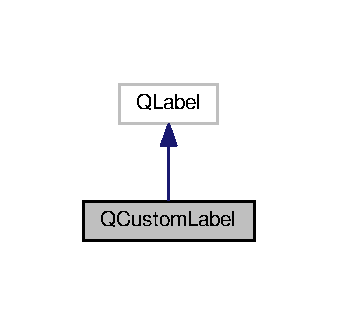
\includegraphics[width=162pt]{classQCustomLabel__inherit__graph}
\end{center}
\end{figure}


Collaboration diagram for Q\-Custom\-Label\-:
\nopagebreak
\begin{figure}[H]
\begin{center}
\leavevmode
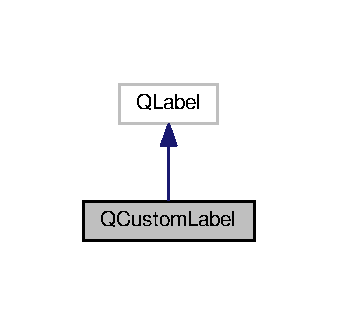
\includegraphics[width=162pt]{classQCustomLabel__coll__graph}
\end{center}
\end{figure}
\subsection*{Signals}
\begin{DoxyCompactItemize}
\item 
\hypertarget{classQCustomLabel_a45deee93a6a40df2979492a2ff680c88}{void {\bfseries Mouse\-\_\-\-Pos} ()}\label{classQCustomLabel_a45deee93a6a40df2979492a2ff680c88}

\item 
\hypertarget{classQCustomLabel_a6c990d236a4ff2e2898a3e84cd130f9b}{void {\bfseries Mouse\-\_\-\-Left\-\_\-\-Pressed} ()}\label{classQCustomLabel_a6c990d236a4ff2e2898a3e84cd130f9b}

\item 
\hypertarget{classQCustomLabel_a221ee1658fe8b86dbcc9036e7b740ab8}{void {\bfseries Mouse\-\_\-\-Right\-\_\-\-Pressed} ()}\label{classQCustomLabel_a221ee1658fe8b86dbcc9036e7b740ab8}

\item 
\hypertarget{classQCustomLabel_a1725399a11e80f0c79f3d1c63cf505ef}{void {\bfseries Mouse\-\_\-\-Release} ()}\label{classQCustomLabel_a1725399a11e80f0c79f3d1c63cf505ef}

\item 
\hypertarget{classQCustomLabel_ae5fe8fd62adb9568cfa6d412d6a62948}{void {\bfseries Mouse\-\_\-\-Left} ()}\label{classQCustomLabel_ae5fe8fd62adb9568cfa6d412d6a62948}

\item 
\hypertarget{classQCustomLabel_aea283ddc963d921271109be3bcb82b6f}{void {\bfseries Mouse\-\_\-\-Scroll} ()}\label{classQCustomLabel_aea283ddc963d921271109be3bcb82b6f}

\item 
\hypertarget{classQCustomLabel_a8c48808fd1d4287bf220df16f7c2feb5}{void {\bfseries Key\-\_\-\-Pressed} ()}\label{classQCustomLabel_a8c48808fd1d4287bf220df16f7c2feb5}

\end{DoxyCompactItemize}
\subsection*{Public Member Functions}
\begin{DoxyCompactItemize}
\item 
\hypertarget{classQCustomLabel_a15eca432ecab522f162c87374ac6bca6}{{\bfseries Q\-Custom\-Label} (Q\-Label $\ast$parent=0)}\label{classQCustomLabel_a15eca432ecab522f162c87374ac6bca6}

\item 
\hypertarget{classQCustomLabel_a834a064e119add6ffb0ff1ea5ce78d7e}{void {\bfseries mouse\-Move\-Event} (Q\-Mouse\-Event $\ast$ev)}\label{classQCustomLabel_a834a064e119add6ffb0ff1ea5ce78d7e}

\item 
\hypertarget{classQCustomLabel_a971a01e5c52150d2874555c5d6b11807}{void {\bfseries mouse\-Press\-Event} (Q\-Mouse\-Event $\ast$ev)}\label{classQCustomLabel_a971a01e5c52150d2874555c5d6b11807}

\item 
\hypertarget{classQCustomLabel_ab88c55fd49219104cfabe91ed68aa496}{void {\bfseries mouse\-Release\-Event} (Q\-Mouse\-Event $\ast$ev)}\label{classQCustomLabel_ab88c55fd49219104cfabe91ed68aa496}

\item 
\hypertarget{classQCustomLabel_a99b5c445f092757d5f1e59c6aee6fb88}{void {\bfseries leave\-Event} (Q\-Event $\ast$ev)}\label{classQCustomLabel_a99b5c445f092757d5f1e59c6aee6fb88}

\item 
\hypertarget{classQCustomLabel_ae7a4aaaf4f56d95199d1279923d7ff92}{void {\bfseries wheel\-Event} (Q\-Wheel\-Event $\ast$ev)}\label{classQCustomLabel_ae7a4aaaf4f56d95199d1279923d7ff92}

\item 
\hypertarget{classQCustomLabel_a38e4ecf9b9298636b36594cdbace5260}{void {\bfseries key\-Press\-Event} (Q\-Key\-Event $\ast$ev)}\label{classQCustomLabel_a38e4ecf9b9298636b36594cdbace5260}

\end{DoxyCompactItemize}
\subsection*{Public Attributes}
\begin{DoxyCompactItemize}
\item 
\hypertarget{classQCustomLabel_a509c6eb2bc4e80ad72901c1afc976b92}{int {\bfseries x}}\label{classQCustomLabel_a509c6eb2bc4e80ad72901c1afc976b92}

\item 
\hypertarget{classQCustomLabel_a3d3309c76e47ccba7101e5504091804c}{int {\bfseries y}}\label{classQCustomLabel_a3d3309c76e47ccba7101e5504091804c}

\item 
\hypertarget{classQCustomLabel_a64b5c030bb65139b76f063de1d0784bf}{int {\bfseries delta}}\label{classQCustomLabel_a64b5c030bb65139b76f063de1d0784bf}

\item 
\hypertarget{classQCustomLabel_a5fa4f875b266bd86a552867e60be86da}{int {\bfseries last\-\_\-left\-\_\-click\-\_\-x}}\label{classQCustomLabel_a5fa4f875b266bd86a552867e60be86da}

\item 
\hypertarget{classQCustomLabel_abb541cfa1a5ceb23f29bc08573838bcd}{int {\bfseries last\-\_\-left\-\_\-click\-\_\-y}}\label{classQCustomLabel_abb541cfa1a5ceb23f29bc08573838bcd}

\item 
\hypertarget{classQCustomLabel_a7b13426cb8aedd2d0af1d55502d61325}{int {\bfseries last\-\_\-right\-\_\-click\-\_\-x}}\label{classQCustomLabel_a7b13426cb8aedd2d0af1d55502d61325}

\item 
\hypertarget{classQCustomLabel_a85b2496bc41541923c82ef03894885a7}{int {\bfseries last\-\_\-right\-\_\-click\-\_\-y}}\label{classQCustomLabel_a85b2496bc41541923c82ef03894885a7}

\end{DoxyCompactItemize}


\subsection{Detailed Description}
This class is a modification of Q\-Label, \hyperlink{classQCustomLabel}{Q\-Custom\-Label} handle events like\-: mouse click, mouse move, scrool wheel move and etc. 

The documentation for this class was generated from the following files\-:\begin{DoxyCompactItemize}
\item 
/home/oscar/\-Desktop/meu\-Fork/\-V\-S\-S-\/\-Vision/src/qcustomlabel.\-h\item 
/home/oscar/\-Desktop/meu\-Fork/\-V\-S\-S-\/\-Vision/src/qcustomlabel.\-cpp\end{DoxyCompactItemize}

\hypertarget{classvss__state_1_1RGB}{}\section{vss\+\_\+state\+:\+:R\+GB Class Reference}
\label{classvss__state_1_1RGB}\index{vss\+\_\+state\+::\+R\+GB@{vss\+\_\+state\+::\+R\+GB}}


Inheritance diagram for vss\+\_\+state\+:\+:R\+GB\+:\nopagebreak
\begin{figure}[H]
\begin{center}
\leavevmode
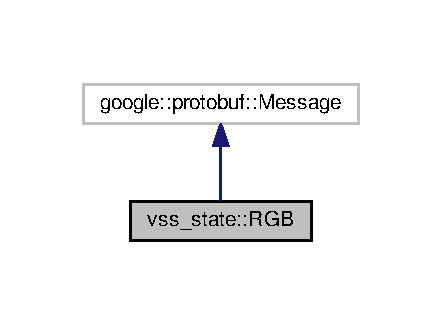
\includegraphics[width=212pt]{classvss__state_1_1RGB__inherit__graph}
\end{center}
\end{figure}


Collaboration diagram for vss\+\_\+state\+:\+:R\+GB\+:\nopagebreak
\begin{figure}[H]
\begin{center}
\leavevmode
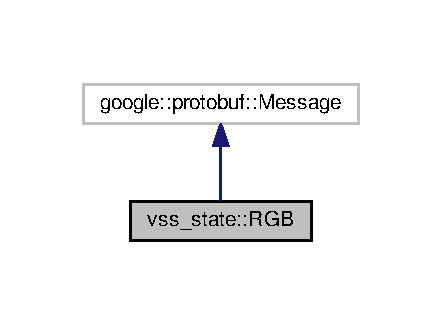
\includegraphics[width=212pt]{classvss__state_1_1RGB__coll__graph}
\end{center}
\end{figure}
\subsection*{Public Member Functions}
\begin{DoxyCompactItemize}
\item 
{\bfseries R\+GB} (const \hyperlink{classvss__state_1_1RGB}{R\+GB} \&from)\hypertarget{classvss__state_1_1RGB_ad057f22713ee486fa88d59661f15c390}{}\label{classvss__state_1_1RGB_ad057f22713ee486fa88d59661f15c390}

\item 
\hyperlink{classvss__state_1_1RGB}{R\+GB} \& {\bfseries operator=} (const \hyperlink{classvss__state_1_1RGB}{R\+GB} \&from)\hypertarget{classvss__state_1_1RGB_ae6850f3550d012f10cb3fe961ceca13a}{}\label{classvss__state_1_1RGB_ae6850f3550d012f10cb3fe961ceca13a}

\item 
const \+::google\+::protobuf\+::\+Unknown\+Field\+Set \& {\bfseries unknown\+\_\+fields} () const \hypertarget{classvss__state_1_1RGB_af3633b5c052c9b983f03dca86c5172e3}{}\label{classvss__state_1_1RGB_af3633b5c052c9b983f03dca86c5172e3}

\item 
inline\+::google\+::protobuf\+::\+Unknown\+Field\+Set $\ast$ {\bfseries mutable\+\_\+unknown\+\_\+fields} ()\hypertarget{classvss__state_1_1RGB_adfdaca9126b92f913d030d86975fb390}{}\label{classvss__state_1_1RGB_adfdaca9126b92f913d030d86975fb390}

\item 
void {\bfseries Swap} (\hyperlink{classvss__state_1_1RGB}{R\+GB} $\ast$other)\hypertarget{classvss__state_1_1RGB_a42f05e54d0dc837400c5079899b463aa}{}\label{classvss__state_1_1RGB_a42f05e54d0dc837400c5079899b463aa}

\item 
\hyperlink{classvss__state_1_1RGB}{R\+GB} $\ast$ {\bfseries New} () const \hypertarget{classvss__state_1_1RGB_a275dd9a86123627063addbde4feb117c}{}\label{classvss__state_1_1RGB_a275dd9a86123627063addbde4feb117c}

\item 
void {\bfseries Copy\+From} (const \+::google\+::protobuf\+::\+Message \&from)\hypertarget{classvss__state_1_1RGB_a7dca7dca78106990bae0191f4fc58aa3}{}\label{classvss__state_1_1RGB_a7dca7dca78106990bae0191f4fc58aa3}

\item 
void {\bfseries Merge\+From} (const \+::google\+::protobuf\+::\+Message \&from)\hypertarget{classvss__state_1_1RGB_a6b287c534b5414da22c85a7ace395032}{}\label{classvss__state_1_1RGB_a6b287c534b5414da22c85a7ace395032}

\item 
void {\bfseries Copy\+From} (const \hyperlink{classvss__state_1_1RGB}{R\+GB} \&from)\hypertarget{classvss__state_1_1RGB_af67ab2848e2357d23f411c0df8bce782}{}\label{classvss__state_1_1RGB_af67ab2848e2357d23f411c0df8bce782}

\item 
void {\bfseries Merge\+From} (const \hyperlink{classvss__state_1_1RGB}{R\+GB} \&from)\hypertarget{classvss__state_1_1RGB_a168e56eb490d40877481d8a709ae8322}{}\label{classvss__state_1_1RGB_a168e56eb490d40877481d8a709ae8322}

\item 
void {\bfseries Clear} ()\hypertarget{classvss__state_1_1RGB_ad0c9a1848a43f2d89ebaa33d51ac6634}{}\label{classvss__state_1_1RGB_ad0c9a1848a43f2d89ebaa33d51ac6634}

\item 
bool {\bfseries Is\+Initialized} () const \hypertarget{classvss__state_1_1RGB_a0d2e0b5f89279b7553ef83d702f0bab8}{}\label{classvss__state_1_1RGB_a0d2e0b5f89279b7553ef83d702f0bab8}

\item 
int {\bfseries Byte\+Size} () const \hypertarget{classvss__state_1_1RGB_a2cd250a169ec6f47428b72537d384bcd}{}\label{classvss__state_1_1RGB_a2cd250a169ec6f47428b72537d384bcd}

\item 
bool {\bfseries Merge\+Partial\+From\+Coded\+Stream} (\+::google\+::protobuf\+::io\+::\+Coded\+Input\+Stream $\ast$input)\hypertarget{classvss__state_1_1RGB_a2e6177a7e8c631c1f62a2d986fdfc452}{}\label{classvss__state_1_1RGB_a2e6177a7e8c631c1f62a2d986fdfc452}

\item 
void {\bfseries Serialize\+With\+Cached\+Sizes} (\+::google\+::protobuf\+::io\+::\+Coded\+Output\+Stream $\ast$output) const \hypertarget{classvss__state_1_1RGB_ab16a3fd0ce7788dd974d078e445e7849}{}\label{classvss__state_1_1RGB_ab16a3fd0ce7788dd974d078e445e7849}

\item 
\+::google\+::protobuf\+::uint8 $\ast$ {\bfseries Serialize\+With\+Cached\+Sizes\+To\+Array} (\+::google\+::protobuf\+::uint8 $\ast$output) const \hypertarget{classvss__state_1_1RGB_a800b57f1540a265138517e52196cc70b}{}\label{classvss__state_1_1RGB_a800b57f1540a265138517e52196cc70b}

\item 
int {\bfseries Get\+Cached\+Size} () const \hypertarget{classvss__state_1_1RGB_a40f2c075e63a05d37dd4023cd25c61e6}{}\label{classvss__state_1_1RGB_a40f2c075e63a05d37dd4023cd25c61e6}

\item 
\+::google\+::protobuf\+::\+Metadata {\bfseries Get\+Metadata} () const \hypertarget{classvss__state_1_1RGB_a72a71c6babca0d3cbd79caf9d8c9c9b2}{}\label{classvss__state_1_1RGB_a72a71c6babca0d3cbd79caf9d8c9c9b2}

\item 
bool {\bfseries has\+\_\+r} () const \hypertarget{classvss__state_1_1RGB_a44a2e2f01894715c2732c8455a27c158}{}\label{classvss__state_1_1RGB_a44a2e2f01894715c2732c8455a27c158}

\item 
void {\bfseries clear\+\_\+r} ()\hypertarget{classvss__state_1_1RGB_acf08083664a7f2da6c10b8faf4b25383}{}\label{classvss__state_1_1RGB_acf08083664a7f2da6c10b8faf4b25383}

\item 
inline\+::google\+::protobuf\+::uint32 {\bfseries r} () const \hypertarget{classvss__state_1_1RGB_ab1fb0a4d6eebeb673bc32c90b1b906ed}{}\label{classvss__state_1_1RGB_ab1fb0a4d6eebeb673bc32c90b1b906ed}

\item 
void {\bfseries set\+\_\+r} (\+::google\+::protobuf\+::uint32 value)\hypertarget{classvss__state_1_1RGB_a33dd755c711c8a7f5a1897e42ea4c711}{}\label{classvss__state_1_1RGB_a33dd755c711c8a7f5a1897e42ea4c711}

\item 
bool {\bfseries has\+\_\+g} () const \hypertarget{classvss__state_1_1RGB_a15f5bdc6f737b63ee48b030fb4348c3a}{}\label{classvss__state_1_1RGB_a15f5bdc6f737b63ee48b030fb4348c3a}

\item 
void {\bfseries clear\+\_\+g} ()\hypertarget{classvss__state_1_1RGB_acb92f198e1d2336c7f76a3aef3fb4cb2}{}\label{classvss__state_1_1RGB_acb92f198e1d2336c7f76a3aef3fb4cb2}

\item 
inline\+::google\+::protobuf\+::uint32 {\bfseries g} () const \hypertarget{classvss__state_1_1RGB_a36c2e8312984ac3b4577c6aae15878b2}{}\label{classvss__state_1_1RGB_a36c2e8312984ac3b4577c6aae15878b2}

\item 
void {\bfseries set\+\_\+g} (\+::google\+::protobuf\+::uint32 value)\hypertarget{classvss__state_1_1RGB_a353c8a4e1ff0d19c5a093b910797c7b9}{}\label{classvss__state_1_1RGB_a353c8a4e1ff0d19c5a093b910797c7b9}

\item 
bool {\bfseries has\+\_\+b} () const \hypertarget{classvss__state_1_1RGB_ad56ba40a1f62f12c828f60042dde4121}{}\label{classvss__state_1_1RGB_ad56ba40a1f62f12c828f60042dde4121}

\item 
void {\bfseries clear\+\_\+b} ()\hypertarget{classvss__state_1_1RGB_a3b8c5f9250f44c8d0f987bcf10abdc64}{}\label{classvss__state_1_1RGB_a3b8c5f9250f44c8d0f987bcf10abdc64}

\item 
inline\+::google\+::protobuf\+::uint32 {\bfseries b} () const \hypertarget{classvss__state_1_1RGB_ac59c6fa5dafec18a115e3a00cd1fa68e}{}\label{classvss__state_1_1RGB_ac59c6fa5dafec18a115e3a00cd1fa68e}

\item 
void {\bfseries set\+\_\+b} (\+::google\+::protobuf\+::uint32 value)\hypertarget{classvss__state_1_1RGB_a3977bb063a529efca387875a69a5b465}{}\label{classvss__state_1_1RGB_a3977bb063a529efca387875a69a5b465}

\end{DoxyCompactItemize}
\subsection*{Static Public Member Functions}
\begin{DoxyCompactItemize}
\item 
static const \+::google\+::protobuf\+::\+Descriptor $\ast$ {\bfseries descriptor} ()\hypertarget{classvss__state_1_1RGB_a64df354aa51e9fb966ee23e03a5e9329}{}\label{classvss__state_1_1RGB_a64df354aa51e9fb966ee23e03a5e9329}

\item 
static const \hyperlink{classvss__state_1_1RGB}{R\+GB} \& {\bfseries default\+\_\+instance} ()\hypertarget{classvss__state_1_1RGB_a82e155d80791f80c397423d539f03614}{}\label{classvss__state_1_1RGB_a82e155d80791f80c397423d539f03614}

\end{DoxyCompactItemize}
\subsection*{Static Public Attributes}
\begin{DoxyCompactItemize}
\item 
static const int {\bfseries k\+R\+Field\+Number} = 1\hypertarget{classvss__state_1_1RGB_a6b14019e7583f983a0dc0e0c713767e5}{}\label{classvss__state_1_1RGB_a6b14019e7583f983a0dc0e0c713767e5}

\item 
static const int {\bfseries k\+G\+Field\+Number} = 2\hypertarget{classvss__state_1_1RGB_a7f4f93a87024582ed9aa94ad501aacc0}{}\label{classvss__state_1_1RGB_a7f4f93a87024582ed9aa94ad501aacc0}

\item 
static const int {\bfseries k\+B\+Field\+Number} = 3\hypertarget{classvss__state_1_1RGB_a2c4583771ba2ee5b0f6798c7ee082b3e}{}\label{classvss__state_1_1RGB_a2c4583771ba2ee5b0f6798c7ee082b3e}

\end{DoxyCompactItemize}
\subsection*{Friends}
\begin{DoxyCompactItemize}
\item 
void {\bfseries protobuf\+\_\+\+Add\+Desc\+\_\+state\+\_\+2eproto} ()\hypertarget{classvss__state_1_1RGB_aab1a2c258f8122a403a979ff57e2a706}{}\label{classvss__state_1_1RGB_aab1a2c258f8122a403a979ff57e2a706}

\item 
void {\bfseries protobuf\+\_\+\+Assign\+Desc\+\_\+state\+\_\+2eproto} ()\hypertarget{classvss__state_1_1RGB_a57d9367bc8a7a94ead11d11194cca1b6}{}\label{classvss__state_1_1RGB_a57d9367bc8a7a94ead11d11194cca1b6}

\item 
void {\bfseries protobuf\+\_\+\+Shutdown\+File\+\_\+state\+\_\+2eproto} ()\hypertarget{classvss__state_1_1RGB_a4e6dc5e8e72799859c4e9556d090e57d}{}\label{classvss__state_1_1RGB_a4e6dc5e8e72799859c4e9556d090e57d}

\end{DoxyCompactItemize}


The documentation for this class was generated from the following files\+:\begin{DoxyCompactItemize}
\item 
/home/johnathan/\+Repositories/\+S\+I\+R\+Lab/\+V\+S\+S-\/\+Vision/src/protos/state.\+pb.\+h\item 
/home/johnathan/\+Repositories/\+S\+I\+R\+Lab/\+V\+S\+S-\/\+Vision/src/protos/state.\+pb.\+cc\end{DoxyCompactItemize}

\hypertarget{structcommon_1_1Robot}{\section{common\-:\-:Robot Struct Reference}
\label{structcommon_1_1Robot}\index{common\-::\-Robot@{common\-::\-Robot}}
}


This strcut represets the pose that one robot can handle. Pos and Vel.  




{\ttfamily \#include $<$common.\-h$>$}



Collaboration diagram for common\-:\-:Robot\-:
\nopagebreak
\begin{figure}[H]
\begin{center}
\leavevmode
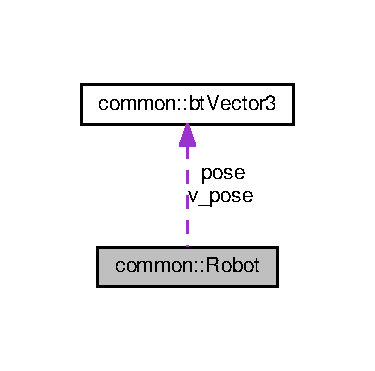
\includegraphics[width=180pt]{structcommon_1_1Robot__coll__graph}
\end{center}
\end{figure}
\subsection*{Public Member Functions}
\begin{DoxyCompactItemize}
\item 
\hypertarget{structcommon_1_1Robot_a41ba088fd67d929808e381126f7b6c2e}{\hyperlink{structcommon_1_1Robot_a41ba088fd67d929808e381126f7b6c2e}{Robot} ()}\label{structcommon_1_1Robot_a41ba088fd67d929808e381126f7b6c2e}

\begin{DoxyCompactList}\small\item\em Default constructor\-: \hyperlink{structcommon_1_1Robot}{Robot} t;. \end{DoxyCompactList}\item 
\hypertarget{structcommon_1_1Robot_a32c611a544e879cf59d66bd87e3884d9}{\hyperlink{structcommon_1_1Robot_a32c611a544e879cf59d66bd87e3884d9}{Robot} (\hyperlink{structcommon_1_1btVector3}{bt\-Vector3} \hyperlink{structcommon_1_1Robot_a31960c8ccd21cde1ca66e263851b83ad}{pose}, \hyperlink{structcommon_1_1btVector3}{bt\-Vector3} \hyperlink{structcommon_1_1Robot_a8114313ba162326a4cb51ce4d5c992f2}{v\-\_\-pose})}\label{structcommon_1_1Robot_a32c611a544e879cf59d66bd87e3884d9}

\begin{DoxyCompactList}\small\item\em Constructor 2\-: \hyperlink{structcommon_1_1Robot}{Robot} t(bt\-Vector3(x, y, yaw), bt\-Vector3(x, y, yaw)) \end{DoxyCompactList}\item 
\hypertarget{structcommon_1_1Robot_a3df83e11a40060ea9d3553384dcdaaa3}{\hyperlink{structcommon_1_1Robot_a3df83e11a40060ea9d3553384dcdaaa3}{Robot} (\hyperlink{structcommon_1_1Robot}{Robot} $\ast$r)}\label{structcommon_1_1Robot_a3df83e11a40060ea9d3553384dcdaaa3}

\begin{DoxyCompactList}\small\item\em Constructor copy\-: \hyperlink{structcommon_1_1Robot}{Robot} t(\-Robot());. \end{DoxyCompactList}\item 
\hypertarget{structcommon_1_1Robot_a224e3f9997e44c5edf67fd0989aee5cf}{void \hyperlink{structcommon_1_1Robot_a224e3f9997e44c5edf67fd0989aee5cf}{show} ()}\label{structcommon_1_1Robot_a224e3f9997e44c5edf67fd0989aee5cf}

\begin{DoxyCompactList}\small\item\em Default function\-: prints all variables. \end{DoxyCompactList}\end{DoxyCompactItemize}
\subsection*{Public Attributes}
\begin{DoxyCompactItemize}
\item 
\hypertarget{structcommon_1_1Robot_a31960c8ccd21cde1ca66e263851b83ad}{\hyperlink{structcommon_1_1btVector3}{bt\-Vector3} \hyperlink{structcommon_1_1Robot_a31960c8ccd21cde1ca66e263851b83ad}{pose}}\label{structcommon_1_1Robot_a31960c8ccd21cde1ca66e263851b83ad}

\begin{DoxyCompactList}\small\item\em Data\-: Pose. \end{DoxyCompactList}\item 
\hypertarget{structcommon_1_1Robot_a8114313ba162326a4cb51ce4d5c992f2}{\hyperlink{structcommon_1_1btVector3}{bt\-Vector3} \hyperlink{structcommon_1_1Robot_a8114313ba162326a4cb51ce4d5c992f2}{v\-\_\-pose}}\label{structcommon_1_1Robot_a8114313ba162326a4cb51ce4d5c992f2}

\begin{DoxyCompactList}\small\item\em Data\-: V\-\_\-\-Pose. \end{DoxyCompactList}\end{DoxyCompactItemize}


\subsection{Detailed Description}
This strcut represets the pose that one robot can handle. Pos and Vel. 

The documentation for this struct was generated from the following file\-:\begin{DoxyCompactItemize}
\item 
/home/oscar/\-Desktop/meu\-Fork/\-V\-S\-S-\/\-Vision/src/common.\-h\end{DoxyCompactItemize}

\hypertarget{classvss__command_1_1Robot__Command}{\section{vss\-\_\-command\-:\-:Robot\-\_\-\-Command Class Reference}
\label{classvss__command_1_1Robot__Command}\index{vss\-\_\-command\-::\-Robot\-\_\-\-Command@{vss\-\_\-command\-::\-Robot\-\_\-\-Command}}
}


Inheritance diagram for vss\-\_\-command\-:\-:Robot\-\_\-\-Command\-:
\nopagebreak
\begin{figure}[H]
\begin{center}
\leavevmode
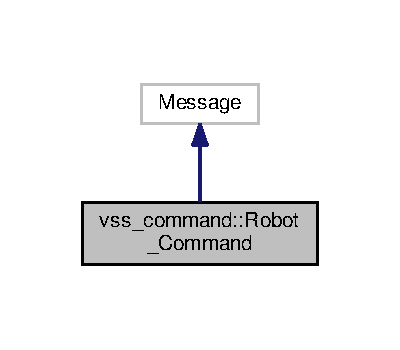
\includegraphics[width=192pt]{classvss__command_1_1Robot__Command__inherit__graph}
\end{center}
\end{figure}


Collaboration diagram for vss\-\_\-command\-:\-:Robot\-\_\-\-Command\-:
\nopagebreak
\begin{figure}[H]
\begin{center}
\leavevmode
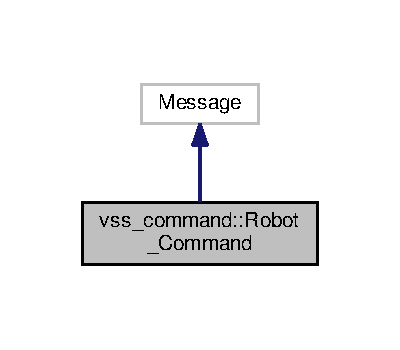
\includegraphics[width=192pt]{classvss__command_1_1Robot__Command__coll__graph}
\end{center}
\end{figure}
\subsection*{Public Member Functions}
\begin{DoxyCompactItemize}
\item 
\hypertarget{classvss__command_1_1Robot__Command_aec1028695262ac9887a661768f2f8bb1}{{\bfseries Robot\-\_\-\-Command} (const \hyperlink{classvss__command_1_1Robot__Command}{Robot\-\_\-\-Command} \&from)}\label{classvss__command_1_1Robot__Command_aec1028695262ac9887a661768f2f8bb1}

\item 
\hypertarget{classvss__command_1_1Robot__Command_afebc3c2ee761027356ce0fabe568ae11}{\hyperlink{classvss__command_1_1Robot__Command}{Robot\-\_\-\-Command} \& {\bfseries operator=} (const \hyperlink{classvss__command_1_1Robot__Command}{Robot\-\_\-\-Command} \&from)}\label{classvss__command_1_1Robot__Command_afebc3c2ee761027356ce0fabe568ae11}

\item 
\hypertarget{classvss__command_1_1Robot__Command_a9df4b6bca5721e6b1ae945dc975af2c6}{const \\*
\-::google\-::protobuf\-::\-Unknown\-Field\-Set \& {\bfseries unknown\-\_\-fields} () const }\label{classvss__command_1_1Robot__Command_a9df4b6bca5721e6b1ae945dc975af2c6}

\item 
\hypertarget{classvss__command_1_1Robot__Command_ac59c88c8dcf9b0e1128e845e238a92d4}{inline\-::google\-::protobuf\-::\-Unknown\-Field\-Set $\ast$ {\bfseries mutable\-\_\-unknown\-\_\-fields} ()}\label{classvss__command_1_1Robot__Command_ac59c88c8dcf9b0e1128e845e238a92d4}

\item 
\hypertarget{classvss__command_1_1Robot__Command_aab4cd2f4e6d3316f414fa32e7ccf1660}{void {\bfseries Swap} (\hyperlink{classvss__command_1_1Robot__Command}{Robot\-\_\-\-Command} $\ast$other)}\label{classvss__command_1_1Robot__Command_aab4cd2f4e6d3316f414fa32e7ccf1660}

\item 
\hypertarget{classvss__command_1_1Robot__Command_a16862f509cc6ad30afa51daa6f18ab73}{\hyperlink{classvss__command_1_1Robot__Command}{Robot\-\_\-\-Command} $\ast$ {\bfseries New} () const }\label{classvss__command_1_1Robot__Command_a16862f509cc6ad30afa51daa6f18ab73}

\item 
\hypertarget{classvss__command_1_1Robot__Command_a44b1cba95f68eb9c9349d1f06b0567db}{void {\bfseries Copy\-From} (const \-::google\-::protobuf\-::\-Message \&from)}\label{classvss__command_1_1Robot__Command_a44b1cba95f68eb9c9349d1f06b0567db}

\item 
\hypertarget{classvss__command_1_1Robot__Command_a72b9a2f6e5fcb0ee33f5c1a5782bb655}{void {\bfseries Merge\-From} (const \-::google\-::protobuf\-::\-Message \&from)}\label{classvss__command_1_1Robot__Command_a72b9a2f6e5fcb0ee33f5c1a5782bb655}

\item 
\hypertarget{classvss__command_1_1Robot__Command_a98f8965b27b6495b2d59dccd8d2bfe19}{void {\bfseries Copy\-From} (const \hyperlink{classvss__command_1_1Robot__Command}{Robot\-\_\-\-Command} \&from)}\label{classvss__command_1_1Robot__Command_a98f8965b27b6495b2d59dccd8d2bfe19}

\item 
\hypertarget{classvss__command_1_1Robot__Command_a48c5d39a8a3d31209db79aa77fcf876f}{void {\bfseries Merge\-From} (const \hyperlink{classvss__command_1_1Robot__Command}{Robot\-\_\-\-Command} \&from)}\label{classvss__command_1_1Robot__Command_a48c5d39a8a3d31209db79aa77fcf876f}

\item 
\hypertarget{classvss__command_1_1Robot__Command_aaffa12def3a1311252dcaccf6becb28b}{void {\bfseries Clear} ()}\label{classvss__command_1_1Robot__Command_aaffa12def3a1311252dcaccf6becb28b}

\item 
\hypertarget{classvss__command_1_1Robot__Command_af368ddcdb8103f40b21503727664fc52}{bool {\bfseries Is\-Initialized} () const }\label{classvss__command_1_1Robot__Command_af368ddcdb8103f40b21503727664fc52}

\item 
\hypertarget{classvss__command_1_1Robot__Command_a54599973bda6814c7842036eb9bf9229}{int {\bfseries Byte\-Size} () const }\label{classvss__command_1_1Robot__Command_a54599973bda6814c7842036eb9bf9229}

\item 
\hypertarget{classvss__command_1_1Robot__Command_a471b2b99a1e476866bdb6ded82d46274}{bool {\bfseries Merge\-Partial\-From\-Coded\-Stream} (\-::google\-::protobuf\-::io\-::\-Coded\-Input\-Stream $\ast$input)}\label{classvss__command_1_1Robot__Command_a471b2b99a1e476866bdb6ded82d46274}

\item 
\hypertarget{classvss__command_1_1Robot__Command_add920699d3f456d9335a4fbacf4a1fa5}{void {\bfseries Serialize\-With\-Cached\-Sizes} (\-::google\-::protobuf\-::io\-::\-Coded\-Output\-Stream $\ast$output) const }\label{classvss__command_1_1Robot__Command_add920699d3f456d9335a4fbacf4a1fa5}

\item 
\hypertarget{classvss__command_1_1Robot__Command_ab3447c593d9b6135979822bad4903648}{\-::google\-::protobuf\-::uint8 $\ast$ {\bfseries Serialize\-With\-Cached\-Sizes\-To\-Array} (\-::google\-::protobuf\-::uint8 $\ast$output) const }\label{classvss__command_1_1Robot__Command_ab3447c593d9b6135979822bad4903648}

\item 
\hypertarget{classvss__command_1_1Robot__Command_a45dc66dc5c38e988073141707b083dae}{int {\bfseries Get\-Cached\-Size} () const }\label{classvss__command_1_1Robot__Command_a45dc66dc5c38e988073141707b083dae}

\item 
\hypertarget{classvss__command_1_1Robot__Command_a5383c49b5b6ef83dc3b9ac3ab2dd870a}{\-::google\-::protobuf\-::\-Metadata {\bfseries Get\-Metadata} () const }\label{classvss__command_1_1Robot__Command_a5383c49b5b6ef83dc3b9ac3ab2dd870a}

\item 
\hypertarget{classvss__command_1_1Robot__Command_ab636015fe88af27ccaf824159805442d}{bool {\bfseries has\-\_\-id} () const }\label{classvss__command_1_1Robot__Command_ab636015fe88af27ccaf824159805442d}

\item 
\hypertarget{classvss__command_1_1Robot__Command_a0b684f61267d6e251f068f1b2a4c772f}{void {\bfseries clear\-\_\-id} ()}\label{classvss__command_1_1Robot__Command_a0b684f61267d6e251f068f1b2a4c772f}

\item 
\hypertarget{classvss__command_1_1Robot__Command_a632b1e7c37152ca3ecca6e45547faa94}{inline\-::google\-::protobuf\-::uint32 {\bfseries id} () const }\label{classvss__command_1_1Robot__Command_a632b1e7c37152ca3ecca6e45547faa94}

\item 
\hypertarget{classvss__command_1_1Robot__Command_a7aa38699c29bd2037112084fbb833efe}{void {\bfseries set\-\_\-id} (\-::google\-::protobuf\-::uint32 value)}\label{classvss__command_1_1Robot__Command_a7aa38699c29bd2037112084fbb833efe}

\item 
\hypertarget{classvss__command_1_1Robot__Command_aba5afdfa1c9844cbea2b8b5c1f9a3a71}{bool {\bfseries has\-\_\-left\-\_\-vel} () const }\label{classvss__command_1_1Robot__Command_aba5afdfa1c9844cbea2b8b5c1f9a3a71}

\item 
\hypertarget{classvss__command_1_1Robot__Command_a728166b3b1a62583a6e46545b5ad44c7}{void {\bfseries clear\-\_\-left\-\_\-vel} ()}\label{classvss__command_1_1Robot__Command_a728166b3b1a62583a6e46545b5ad44c7}

\item 
\hypertarget{classvss__command_1_1Robot__Command_a179ef683cadb10827e8112f2f1e174a5}{float {\bfseries left\-\_\-vel} () const }\label{classvss__command_1_1Robot__Command_a179ef683cadb10827e8112f2f1e174a5}

\item 
\hypertarget{classvss__command_1_1Robot__Command_a2792ed641e6a25348fab7d26d989f670}{void {\bfseries set\-\_\-left\-\_\-vel} (float value)}\label{classvss__command_1_1Robot__Command_a2792ed641e6a25348fab7d26d989f670}

\item 
\hypertarget{classvss__command_1_1Robot__Command_af192678ad6c73ff034b042275511d503}{bool {\bfseries has\-\_\-right\-\_\-vel} () const }\label{classvss__command_1_1Robot__Command_af192678ad6c73ff034b042275511d503}

\item 
\hypertarget{classvss__command_1_1Robot__Command_acdb3ec06b0b7183f192df01af72e70aa}{void {\bfseries clear\-\_\-right\-\_\-vel} ()}\label{classvss__command_1_1Robot__Command_acdb3ec06b0b7183f192df01af72e70aa}

\item 
\hypertarget{classvss__command_1_1Robot__Command_ad8e37a453b8729183b59a2bade49cc74}{float {\bfseries right\-\_\-vel} () const }\label{classvss__command_1_1Robot__Command_ad8e37a453b8729183b59a2bade49cc74}

\item 
\hypertarget{classvss__command_1_1Robot__Command_a6e63f0df3268bde40f11d47ea167ceb3}{void {\bfseries set\-\_\-right\-\_\-vel} (float value)}\label{classvss__command_1_1Robot__Command_a6e63f0df3268bde40f11d47ea167ceb3}

\end{DoxyCompactItemize}
\subsection*{Static Public Member Functions}
\begin{DoxyCompactItemize}
\item 
\hypertarget{classvss__command_1_1Robot__Command_ad40c6b295898b078ff34e9966d89b6e5}{static const \\*
\-::google\-::protobuf\-::\-Descriptor $\ast$ {\bfseries descriptor} ()}\label{classvss__command_1_1Robot__Command_ad40c6b295898b078ff34e9966d89b6e5}

\item 
\hypertarget{classvss__command_1_1Robot__Command_a4c818a68a4bee11acbc7e7b5483ff4d7}{static const \hyperlink{classvss__command_1_1Robot__Command}{Robot\-\_\-\-Command} \& {\bfseries default\-\_\-instance} ()}\label{classvss__command_1_1Robot__Command_a4c818a68a4bee11acbc7e7b5483ff4d7}

\end{DoxyCompactItemize}
\subsection*{Static Public Attributes}
\begin{DoxyCompactItemize}
\item 
\hypertarget{classvss__command_1_1Robot__Command_a72d358bc06840eb9b5835ad46cee4620}{static const int {\bfseries k\-Id\-Field\-Number} = 1}\label{classvss__command_1_1Robot__Command_a72d358bc06840eb9b5835ad46cee4620}

\item 
\hypertarget{classvss__command_1_1Robot__Command_a834467a27672508216892c745d78bad4}{static const int {\bfseries k\-Left\-Vel\-Field\-Number} = 2}\label{classvss__command_1_1Robot__Command_a834467a27672508216892c745d78bad4}

\item 
\hypertarget{classvss__command_1_1Robot__Command_adb4e9f137218f7bf68ba93029e028e40}{static const int {\bfseries k\-Right\-Vel\-Field\-Number} = 3}\label{classvss__command_1_1Robot__Command_adb4e9f137218f7bf68ba93029e028e40}

\end{DoxyCompactItemize}
\subsection*{Friends}
\begin{DoxyCompactItemize}
\item 
\hypertarget{classvss__command_1_1Robot__Command_a4825d92f856fcb4b02c67b601c433796}{void {\bfseries protobuf\-\_\-\-Add\-Desc\-\_\-command\-\_\-2eproto} ()}\label{classvss__command_1_1Robot__Command_a4825d92f856fcb4b02c67b601c433796}

\item 
\hypertarget{classvss__command_1_1Robot__Command_a4c6fb97c25079d49daf010087d869100}{void {\bfseries protobuf\-\_\-\-Assign\-Desc\-\_\-command\-\_\-2eproto} ()}\label{classvss__command_1_1Robot__Command_a4c6fb97c25079d49daf010087d869100}

\item 
\hypertarget{classvss__command_1_1Robot__Command_a4cf10633ad46690f5eec6bdbbcf62de0}{void {\bfseries protobuf\-\_\-\-Shutdown\-File\-\_\-command\-\_\-2eproto} ()}\label{classvss__command_1_1Robot__Command_a4cf10633ad46690f5eec6bdbbcf62de0}

\end{DoxyCompactItemize}


The documentation for this class was generated from the following files\-:\begin{DoxyCompactItemize}
\item 
/home/oscar/\-Desktop/meu\-Fork/\-V\-S\-S-\/\-Vision/src/protos/command.\-pb.\-h\item 
/home/oscar/\-Desktop/meu\-Fork/\-V\-S\-S-\/\-Vision/src/protos/command.\-pb.\-cc\end{DoxyCompactItemize}

\hypertarget{classvss__state_1_1Robot__State}{}\section{vss\+\_\+state\+:\+:Robot\+\_\+\+State Class Reference}
\label{classvss__state_1_1Robot__State}\index{vss\+\_\+state\+::\+Robot\+\_\+\+State@{vss\+\_\+state\+::\+Robot\+\_\+\+State}}


Inheritance diagram for vss\+\_\+state\+:\+:Robot\+\_\+\+State\+:\nopagebreak
\begin{figure}[H]
\begin{center}
\leavevmode
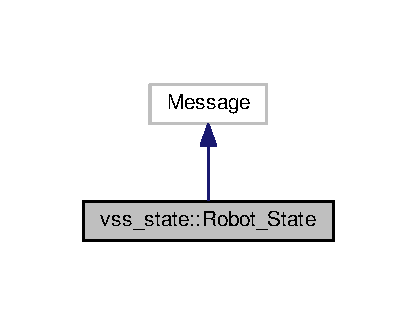
\includegraphics[width=200pt]{classvss__state_1_1Robot__State__inherit__graph}
\end{center}
\end{figure}


Collaboration diagram for vss\+\_\+state\+:\+:Robot\+\_\+\+State\+:\nopagebreak
\begin{figure}[H]
\begin{center}
\leavevmode
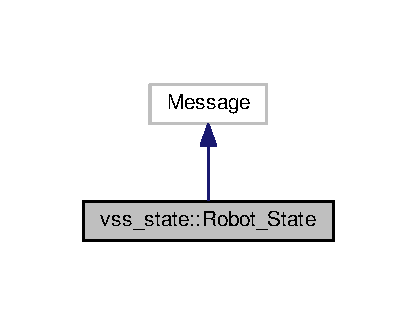
\includegraphics[width=200pt]{classvss__state_1_1Robot__State__coll__graph}
\end{center}
\end{figure}
\subsection*{Public Member Functions}
\begin{DoxyCompactItemize}
\item 
{\bfseries Robot\+\_\+\+State} (const \hyperlink{classvss__state_1_1Robot__State}{Robot\+\_\+\+State} \&from)\hypertarget{classvss__state_1_1Robot__State_a067b968ee504ea53efd93d9aa27c96ca}{}\label{classvss__state_1_1Robot__State_a067b968ee504ea53efd93d9aa27c96ca}

\item 
\hyperlink{classvss__state_1_1Robot__State}{Robot\+\_\+\+State} \& {\bfseries operator=} (const \hyperlink{classvss__state_1_1Robot__State}{Robot\+\_\+\+State} \&from)\hypertarget{classvss__state_1_1Robot__State_ad37aa84870eea581e0406cfb5db502ac}{}\label{classvss__state_1_1Robot__State_ad37aa84870eea581e0406cfb5db502ac}

\item 
const \+::google\+::protobuf\+::\+Unknown\+Field\+Set \& {\bfseries unknown\+\_\+fields} () const \hypertarget{classvss__state_1_1Robot__State_a12a57833a931bfb941527d777fb1d99a}{}\label{classvss__state_1_1Robot__State_a12a57833a931bfb941527d777fb1d99a}

\item 
inline\+::google\+::protobuf\+::\+Unknown\+Field\+Set $\ast$ {\bfseries mutable\+\_\+unknown\+\_\+fields} ()\hypertarget{classvss__state_1_1Robot__State_adda3db07f10ebdb69699bb992976ace3}{}\label{classvss__state_1_1Robot__State_adda3db07f10ebdb69699bb992976ace3}

\item 
void {\bfseries Swap} (\hyperlink{classvss__state_1_1Robot__State}{Robot\+\_\+\+State} $\ast$other)\hypertarget{classvss__state_1_1Robot__State_a4f0475b13ab71a00c88f4662e82decea}{}\label{classvss__state_1_1Robot__State_a4f0475b13ab71a00c88f4662e82decea}

\item 
\hyperlink{classvss__state_1_1Robot__State}{Robot\+\_\+\+State} $\ast$ {\bfseries New} () const \hypertarget{classvss__state_1_1Robot__State_a1ae61a4d15e74bd8210d8943b4cb4d93}{}\label{classvss__state_1_1Robot__State_a1ae61a4d15e74bd8210d8943b4cb4d93}

\item 
void {\bfseries Copy\+From} (const \+::google\+::protobuf\+::\+Message \&from)\hypertarget{classvss__state_1_1Robot__State_ad8ff7bd295e28703ef3b6bdc6dba1435}{}\label{classvss__state_1_1Robot__State_ad8ff7bd295e28703ef3b6bdc6dba1435}

\item 
void {\bfseries Merge\+From} (const \+::google\+::protobuf\+::\+Message \&from)\hypertarget{classvss__state_1_1Robot__State_a5f5cb63411c8f37399dfd169c94e6e54}{}\label{classvss__state_1_1Robot__State_a5f5cb63411c8f37399dfd169c94e6e54}

\item 
void {\bfseries Copy\+From} (const \hyperlink{classvss__state_1_1Robot__State}{Robot\+\_\+\+State} \&from)\hypertarget{classvss__state_1_1Robot__State_a4e18e564b9c470d6f382c8c1c040cfb4}{}\label{classvss__state_1_1Robot__State_a4e18e564b9c470d6f382c8c1c040cfb4}

\item 
void {\bfseries Merge\+From} (const \hyperlink{classvss__state_1_1Robot__State}{Robot\+\_\+\+State} \&from)\hypertarget{classvss__state_1_1Robot__State_a66fadfccfb89ba8742bafa6cd9597420}{}\label{classvss__state_1_1Robot__State_a66fadfccfb89ba8742bafa6cd9597420}

\item 
void {\bfseries Clear} ()\hypertarget{classvss__state_1_1Robot__State_a78f3f24cbb0f2e1fac867550bf05da91}{}\label{classvss__state_1_1Robot__State_a78f3f24cbb0f2e1fac867550bf05da91}

\item 
bool {\bfseries Is\+Initialized} () const \hypertarget{classvss__state_1_1Robot__State_ae482d98ba51e51887efe37a4d2f6abb5}{}\label{classvss__state_1_1Robot__State_ae482d98ba51e51887efe37a4d2f6abb5}

\item 
int {\bfseries Byte\+Size} () const \hypertarget{classvss__state_1_1Robot__State_a6ff13cd34434ab985d2b560a13219532}{}\label{classvss__state_1_1Robot__State_a6ff13cd34434ab985d2b560a13219532}

\item 
bool {\bfseries Merge\+Partial\+From\+Coded\+Stream} (\+::google\+::protobuf\+::io\+::\+Coded\+Input\+Stream $\ast$input)\hypertarget{classvss__state_1_1Robot__State_a82a0f5270a13c5211d94c6da6726ab8d}{}\label{classvss__state_1_1Robot__State_a82a0f5270a13c5211d94c6da6726ab8d}

\item 
void {\bfseries Serialize\+With\+Cached\+Sizes} (\+::google\+::protobuf\+::io\+::\+Coded\+Output\+Stream $\ast$output) const \hypertarget{classvss__state_1_1Robot__State_a67b812e24a55cdfad4d58049f8e0e674}{}\label{classvss__state_1_1Robot__State_a67b812e24a55cdfad4d58049f8e0e674}

\item 
\+::google\+::protobuf\+::uint8 $\ast$ {\bfseries Serialize\+With\+Cached\+Sizes\+To\+Array} (\+::google\+::protobuf\+::uint8 $\ast$output) const \hypertarget{classvss__state_1_1Robot__State_a2a833a548c45c6e25eaba0e9855ed563}{}\label{classvss__state_1_1Robot__State_a2a833a548c45c6e25eaba0e9855ed563}

\item 
int {\bfseries Get\+Cached\+Size} () const \hypertarget{classvss__state_1_1Robot__State_ada89e91697c3773ab009c765b2884734}{}\label{classvss__state_1_1Robot__State_ada89e91697c3773ab009c765b2884734}

\item 
\+::google\+::protobuf\+::\+Metadata {\bfseries Get\+Metadata} () const \hypertarget{classvss__state_1_1Robot__State_afb2668f8b861828a30ac978ab416e900}{}\label{classvss__state_1_1Robot__State_afb2668f8b861828a30ac978ab416e900}

\item 
bool {\bfseries has\+\_\+x} () const \hypertarget{classvss__state_1_1Robot__State_a09fac3756dfc7062c51589ae93647843}{}\label{classvss__state_1_1Robot__State_a09fac3756dfc7062c51589ae93647843}

\item 
void {\bfseries clear\+\_\+x} ()\hypertarget{classvss__state_1_1Robot__State_aed7c83e7e762fe8c0dbb5219ab2ad911}{}\label{classvss__state_1_1Robot__State_aed7c83e7e762fe8c0dbb5219ab2ad911}

\item 
float {\bfseries x} () const \hypertarget{classvss__state_1_1Robot__State_a7a66c2bef1cf33e857a12870257a88c6}{}\label{classvss__state_1_1Robot__State_a7a66c2bef1cf33e857a12870257a88c6}

\item 
void {\bfseries set\+\_\+x} (float value)\hypertarget{classvss__state_1_1Robot__State_ae3697f12fff4a9012754e791d4a80395}{}\label{classvss__state_1_1Robot__State_ae3697f12fff4a9012754e791d4a80395}

\item 
bool {\bfseries has\+\_\+y} () const \hypertarget{classvss__state_1_1Robot__State_a7a6bb8e6be693ba9bdafc990a1aeb3e0}{}\label{classvss__state_1_1Robot__State_a7a6bb8e6be693ba9bdafc990a1aeb3e0}

\item 
void {\bfseries clear\+\_\+y} ()\hypertarget{classvss__state_1_1Robot__State_aba9e62ec76d46a6f48fab72686c25491}{}\label{classvss__state_1_1Robot__State_aba9e62ec76d46a6f48fab72686c25491}

\item 
float {\bfseries y} () const \hypertarget{classvss__state_1_1Robot__State_a1b874baedd64730abd6043e39c2f78b1}{}\label{classvss__state_1_1Robot__State_a1b874baedd64730abd6043e39c2f78b1}

\item 
void {\bfseries set\+\_\+y} (float value)\hypertarget{classvss__state_1_1Robot__State_a06c124cc4ea79f31def60bb66adf86fb}{}\label{classvss__state_1_1Robot__State_a06c124cc4ea79f31def60bb66adf86fb}

\item 
bool {\bfseries has\+\_\+color} () const \hypertarget{classvss__state_1_1Robot__State_a319868975523f46fce84fedda26c478e}{}\label{classvss__state_1_1Robot__State_a319868975523f46fce84fedda26c478e}

\item 
void {\bfseries clear\+\_\+color} ()\hypertarget{classvss__state_1_1Robot__State_a0d95199c67056fd8a0b6bb873d278392}{}\label{classvss__state_1_1Robot__State_a0d95199c67056fd8a0b6bb873d278392}

\item 
const \+::\hyperlink{classvss__state_1_1RGB}{vss\+\_\+state\+::\+R\+GB} \& {\bfseries color} () const \hypertarget{classvss__state_1_1Robot__State_a1e8b02c137ceae1f7a875bdf5371aa91}{}\label{classvss__state_1_1Robot__State_a1e8b02c137ceae1f7a875bdf5371aa91}

\item 
inline\+::vss\+\_\+state\+::\+R\+GB $\ast$ {\bfseries mutable\+\_\+color} ()\hypertarget{classvss__state_1_1Robot__State_aa91b85fa199de6f9b4673529f86f1d01}{}\label{classvss__state_1_1Robot__State_aa91b85fa199de6f9b4673529f86f1d01}

\item 
inline\+::vss\+\_\+state\+::\+R\+GB $\ast$ {\bfseries release\+\_\+color} ()\hypertarget{classvss__state_1_1Robot__State_aba8a8ff5aa02a978e3ff2e8b6335f0ce}{}\label{classvss__state_1_1Robot__State_aba8a8ff5aa02a978e3ff2e8b6335f0ce}

\item 
void {\bfseries set\+\_\+allocated\+\_\+color} (\+::\hyperlink{classvss__state_1_1RGB}{vss\+\_\+state\+::\+R\+GB} $\ast$color)\hypertarget{classvss__state_1_1Robot__State_a368a1f90ce946cd075aa050885e1e6d3}{}\label{classvss__state_1_1Robot__State_a368a1f90ce946cd075aa050885e1e6d3}

\item 
bool {\bfseries has\+\_\+yaw} () const \hypertarget{classvss__state_1_1Robot__State_a7f07f9c8c553babff64eb056a103c189}{}\label{classvss__state_1_1Robot__State_a7f07f9c8c553babff64eb056a103c189}

\item 
void {\bfseries clear\+\_\+yaw} ()\hypertarget{classvss__state_1_1Robot__State_a1f023fdc194aea61557b0cba586e3b1a}{}\label{classvss__state_1_1Robot__State_a1f023fdc194aea61557b0cba586e3b1a}

\item 
float {\bfseries yaw} () const \hypertarget{classvss__state_1_1Robot__State_a16a51084f1e143e9cc0eff17991f42fe}{}\label{classvss__state_1_1Robot__State_a16a51084f1e143e9cc0eff17991f42fe}

\item 
void {\bfseries set\+\_\+yaw} (float value)\hypertarget{classvss__state_1_1Robot__State_a80d78f0f346441c0e0407ff6503ee3eb}{}\label{classvss__state_1_1Robot__State_a80d78f0f346441c0e0407ff6503ee3eb}

\end{DoxyCompactItemize}
\subsection*{Static Public Member Functions}
\begin{DoxyCompactItemize}
\item 
static const \+::google\+::protobuf\+::\+Descriptor $\ast$ {\bfseries descriptor} ()\hypertarget{classvss__state_1_1Robot__State_af15c0b33b2edbd683bfb87c76e9b94b7}{}\label{classvss__state_1_1Robot__State_af15c0b33b2edbd683bfb87c76e9b94b7}

\item 
static const \hyperlink{classvss__state_1_1Robot__State}{Robot\+\_\+\+State} \& {\bfseries default\+\_\+instance} ()\hypertarget{classvss__state_1_1Robot__State_aa14ffa0e9a4e47e1c824b2c82039b02c}{}\label{classvss__state_1_1Robot__State_aa14ffa0e9a4e47e1c824b2c82039b02c}

\end{DoxyCompactItemize}
\subsection*{Static Public Attributes}
\begin{DoxyCompactItemize}
\item 
static const int {\bfseries k\+X\+Field\+Number} = 1\hypertarget{classvss__state_1_1Robot__State_a928f084cd2d0fc573071b7193e0c7c0a}{}\label{classvss__state_1_1Robot__State_a928f084cd2d0fc573071b7193e0c7c0a}

\item 
static const int {\bfseries k\+Y\+Field\+Number} = 2\hypertarget{classvss__state_1_1Robot__State_a17b26fab9fee8484866c751fb2f36325}{}\label{classvss__state_1_1Robot__State_a17b26fab9fee8484866c751fb2f36325}

\item 
static const int {\bfseries k\+Color\+Field\+Number} = 3\hypertarget{classvss__state_1_1Robot__State_a941074e9004ce28bc7cddfd36aeacb43}{}\label{classvss__state_1_1Robot__State_a941074e9004ce28bc7cddfd36aeacb43}

\item 
static const int {\bfseries k\+Yaw\+Field\+Number} = 4\hypertarget{classvss__state_1_1Robot__State_a1a2ca06cd76b5f7343198d45237a9727}{}\label{classvss__state_1_1Robot__State_a1a2ca06cd76b5f7343198d45237a9727}

\end{DoxyCompactItemize}
\subsection*{Friends}
\begin{DoxyCompactItemize}
\item 
void {\bfseries protobuf\+\_\+\+Add\+Desc\+\_\+state\+\_\+2eproto} ()\hypertarget{classvss__state_1_1Robot__State_aab1a2c258f8122a403a979ff57e2a706}{}\label{classvss__state_1_1Robot__State_aab1a2c258f8122a403a979ff57e2a706}

\item 
void {\bfseries protobuf\+\_\+\+Assign\+Desc\+\_\+state\+\_\+2eproto} ()\hypertarget{classvss__state_1_1Robot__State_a57d9367bc8a7a94ead11d11194cca1b6}{}\label{classvss__state_1_1Robot__State_a57d9367bc8a7a94ead11d11194cca1b6}

\item 
void {\bfseries protobuf\+\_\+\+Shutdown\+File\+\_\+state\+\_\+2eproto} ()\hypertarget{classvss__state_1_1Robot__State_a4e6dc5e8e72799859c4e9556d090e57d}{}\label{classvss__state_1_1Robot__State_a4e6dc5e8e72799859c4e9556d090e57d}

\end{DoxyCompactItemize}


The documentation for this class was generated from the following files\+:\begin{DoxyCompactItemize}
\item 
/home/johnathan/\+Repositories/\+S\+I\+R\+Lab/\+V\+S\+S-\/\+Vision/src/protos/state.\+pb.\+h\item 
/home/johnathan/\+Repositories/\+S\+I\+R\+Lab/\+V\+S\+S-\/\+Vision/src/protos/state.\+pb.\+cc\end{DoxyCompactItemize}

\hypertarget{classSQLite}{}\section{S\+Q\+Lite Class Reference}
\label{classSQLite}\index{S\+Q\+Lite@{S\+Q\+Lite}}
\subsection*{Public Member Functions}
\begin{DoxyCompactItemize}
\item 
{\bfseries S\+Q\+Lite} (string, string)\hypertarget{classSQLite_aec016ee26d918bb715383b7578118166}{}\label{classSQLite_aec016ee26d918bb715383b7578118166}

\item 
void {\bfseries open} ()\hypertarget{classSQLite_a2ba6d61d356aac7b2a0d7323ba997279}{}\label{classSQLite_a2ba6d61d356aac7b2a0d7323ba997279}

\item 
void {\bfseries close} ()\hypertarget{classSQLite_aac5338faf7580f6adb3560c91d58b54a}{}\label{classSQLite_aac5338faf7580f6adb3560c91d58b54a}

\item 
void {\bfseries insert\+\_\+calibration} ()\hypertarget{classSQLite_ae145e41fed72678f0e2900ec093ad323}{}\label{classSQLite_ae145e41fed72678f0e2900ec093ad323}

\item 
void {\bfseries select\+\_\+calibration} (string s=\char`\"{}\char`\"{})\hypertarget{classSQLite_aeb720971a449cc51d124251fa995cb5c}{}\label{classSQLite_aeb720971a449cc51d124251fa995cb5c}

\end{DoxyCompactItemize}
\subsection*{Protected Member Functions}
\begin{DoxyCompactItemize}
\item 
void {\bfseries clean\+\_\+query} ()\hypertarget{classSQLite_a3b7e7d4f78e02266bd7bb9b6eb4828ee}{}\label{classSQLite_a3b7e7d4f78e02266bd7bb9b6eb4828ee}

\end{DoxyCompactItemize}
\subsection*{Static Protected Member Functions}
\begin{DoxyCompactItemize}
\item 
static int {\bfseries callback} (void $\ast$Not\+Used, int argc, char $\ast$$\ast$argv, char $\ast$$\ast$az\+Col\+Name)\hypertarget{classSQLite_a2cdec2824226fb74b9c5f53fb2eb9c52}{}\label{classSQLite_a2cdec2824226fb74b9c5f53fb2eb9c52}

\end{DoxyCompactItemize}
\subsection*{Protected Attributes}
\begin{DoxyCompactItemize}
\item 
sqlite3 $\ast$ {\bfseries db}\hypertarget{classSQLite_a1d24b48aa333500d31dd1741c474ee77}{}\label{classSQLite_a1d24b48aa333500d31dd1741c474ee77}

\item 
string {\bfseries path\+\_\+database}\hypertarget{classSQLite_a35c90bc05faa587c66031661a365db20}{}\label{classSQLite_a35c90bc05faa587c66031661a365db20}

\item 
string {\bfseries password}\hypertarget{classSQLite_a5db7ea6ca4da520fb5125631b081acb9}{}\label{classSQLite_a5db7ea6ca4da520fb5125631b081acb9}

\item 
stringstream {\bfseries query}\hypertarget{classSQLite_a524b7fb749c55eae9076981de81f6576}{}\label{classSQLite_a524b7fb749c55eae9076981de81f6576}

\item 
int {\bfseries status\+\_\+db}\hypertarget{classSQLite_ab54d46b70b16ac3d91631c926d633d42}{}\label{classSQLite_ab54d46b70b16ac3d91631c926d633d42}

\item 
char $\ast$ {\bfseries error\+\_\+query}\hypertarget{classSQLite_a641bc6c63769eee5ab03dfd0cd26f0bc}{}\label{classSQLite_a641bc6c63769eee5ab03dfd0cd26f0bc}

\item 
const char $\ast$ {\bfseries data}\hypertarget{classSQLite_a7c608c690c08fce28810d549ab488074}{}\label{classSQLite_a7c608c690c08fce28810d549ab488074}

\end{DoxyCompactItemize}


The documentation for this class was generated from the following files\+:\begin{DoxyCompactItemize}
\item 
/home/johnathan/\+Repositories/\+S\+I\+R\+Lab/\+V\+S\+S-\/\+Vision/src/sqlite.\+h\item 
/home/johnathan/\+Repositories/\+S\+I\+R\+Lab/\+V\+S\+S-\/\+Vision/src/sqlite.\+cpp\end{DoxyCompactItemize}

\hypertarget{structcommon_1_1State}{}\section{common\+:\+:State Struct Reference}
\label{structcommon_1_1State}\index{common\+::\+State@{common\+::\+State}}


This struct represents the state that the workspace can handle.  




{\ttfamily \#include $<$common.\+h$>$}



Collaboration diagram for common\+:\+:State\+:\nopagebreak
\begin{figure}[H]
\begin{center}
\leavevmode
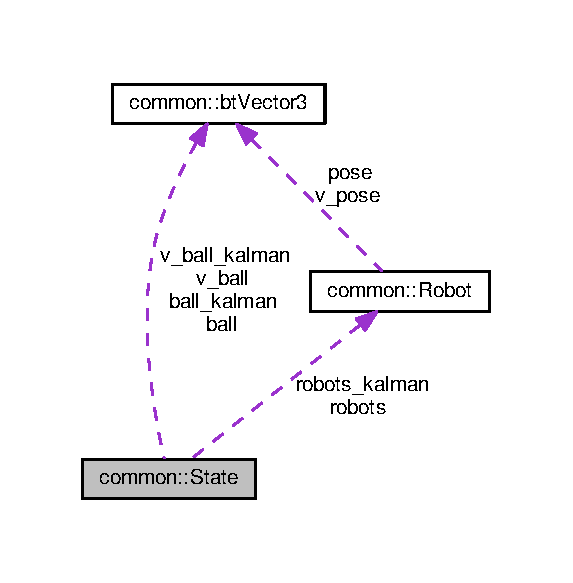
\includegraphics[width=276pt]{structcommon_1_1State__coll__graph}
\end{center}
\end{figure}
\subsection*{Public Member Functions}
\begin{DoxyCompactItemize}
\item 
\hyperlink{structcommon_1_1State_ac8dcfb15646bb310c85161de2900c8c6}{State} ()\hypertarget{structcommon_1_1State_ac8dcfb15646bb310c85161de2900c8c6}{}\label{structcommon_1_1State_ac8dcfb15646bb310c85161de2900c8c6}

\begin{DoxyCompactList}\small\item\em Default constructor\+: \hyperlink{structcommon_1_1State}{State} s;. \end{DoxyCompactList}\item 
void \hyperlink{structcommon_1_1State_af0a474961bf0f3afe274ce27da0f28a3}{show} ()\hypertarget{structcommon_1_1State_af0a474961bf0f3afe274ce27da0f28a3}{}\label{structcommon_1_1State_af0a474961bf0f3afe274ce27da0f28a3}

\begin{DoxyCompactList}\small\item\em Default function\+: prints all variables. \end{DoxyCompactList}\end{DoxyCompactItemize}
\subsection*{Public Attributes}
\begin{DoxyCompactItemize}
\item 
\hyperlink{structcommon_1_1Robot}{Robot} \hyperlink{structcommon_1_1State_a675b02202e4cc1c08408ea4d348ae84b}{robots} \mbox{[}6\mbox{]}\hypertarget{structcommon_1_1State_a675b02202e4cc1c08408ea4d348ae84b}{}\label{structcommon_1_1State_a675b02202e4cc1c08408ea4d348ae84b}

\begin{DoxyCompactList}\small\item\em All robots by vision. \end{DoxyCompactList}\item 
\hyperlink{structcommon_1_1Robot}{Robot} \hyperlink{structcommon_1_1State_aac577c6d23eb389042327ca7026ab1c1}{robots\+\_\+kalman} \mbox{[}6\mbox{]}\hypertarget{structcommon_1_1State_aac577c6d23eb389042327ca7026ab1c1}{}\label{structcommon_1_1State_aac577c6d23eb389042327ca7026ab1c1}

\begin{DoxyCompactList}\small\item\em All robots by kalman. \end{DoxyCompactList}\item 
\hyperlink{structcommon_1_1btVector3}{bt\+Vector3} \hyperlink{structcommon_1_1State_ac4c33250cf2ef39fd319a64f0d51c7bd}{ball}\hypertarget{structcommon_1_1State_ac4c33250cf2ef39fd319a64f0d51c7bd}{}\label{structcommon_1_1State_ac4c33250cf2ef39fd319a64f0d51c7bd}

\begin{DoxyCompactList}\small\item\em Pos ball by vision. \end{DoxyCompactList}\item 
\hyperlink{structcommon_1_1btVector3}{bt\+Vector3} \hyperlink{structcommon_1_1State_af909736805817197988afad7f5b20a9f}{v\+\_\+ball}\hypertarget{structcommon_1_1State_af909736805817197988afad7f5b20a9f}{}\label{structcommon_1_1State_af909736805817197988afad7f5b20a9f}

\begin{DoxyCompactList}\small\item\em Vel ball by vision. \end{DoxyCompactList}\item 
\hyperlink{structcommon_1_1btVector3}{bt\+Vector3} \hyperlink{structcommon_1_1State_ab6b6487077c6bf6fd8f308ad592c6470}{ball\+\_\+kalman}\hypertarget{structcommon_1_1State_ab6b6487077c6bf6fd8f308ad592c6470}{}\label{structcommon_1_1State_ab6b6487077c6bf6fd8f308ad592c6470}

\begin{DoxyCompactList}\small\item\em Pos ball by kalman. \end{DoxyCompactList}\item 
\hyperlink{structcommon_1_1btVector3}{bt\+Vector3} \hyperlink{structcommon_1_1State_adc2d51526dffd90f889324c90fa082a0}{v\+\_\+ball\+\_\+kalman}\hypertarget{structcommon_1_1State_adc2d51526dffd90f889324c90fa082a0}{}\label{structcommon_1_1State_adc2d51526dffd90f889324c90fa082a0}

\begin{DoxyCompactList}\small\item\em Vel ball by kalman. \end{DoxyCompactList}\end{DoxyCompactItemize}


\subsection{Detailed Description}
This struct represents the state that the workspace can handle. 

The documentation for this struct was generated from the following file\+:\begin{DoxyCompactItemize}
\item 
/home/johnathan/\+Repositories/\+S\+I\+R\+Lab/\+V\+S\+S-\/\+Vision/src/common.\+h\end{DoxyCompactItemize}

\hypertarget{structvss__command_1_1StaticDescriptorInitializer__command__2eproto}{\section{vss\-\_\-command\-:\-:Static\-Descriptor\-Initializer\-\_\-command\-\_\-2eproto Struct Reference}
\label{structvss__command_1_1StaticDescriptorInitializer__command__2eproto}\index{vss\-\_\-command\-::\-Static\-Descriptor\-Initializer\-\_\-command\-\_\-2eproto@{vss\-\_\-command\-::\-Static\-Descriptor\-Initializer\-\_\-command\-\_\-2eproto}}
}


The documentation for this struct was generated from the following file\-:\begin{DoxyCompactItemize}
\item 
/home/sirlab/\-Repositorios/\-S\-I\-R\-Lab/\-V\-S\-S-\/\-Vision/src/protos/command.\-pb.\-cc\end{DoxyCompactItemize}

\hypertarget{structvss__state_1_1StaticDescriptorInitializer__state__2eproto}{\section{vss\-\_\-state\-:\-:Static\-Descriptor\-Initializer\-\_\-state\-\_\-2eproto Struct Reference}
\label{structvss__state_1_1StaticDescriptorInitializer__state__2eproto}\index{vss\-\_\-state\-::\-Static\-Descriptor\-Initializer\-\_\-state\-\_\-2eproto@{vss\-\_\-state\-::\-Static\-Descriptor\-Initializer\-\_\-state\-\_\-2eproto}}
}


The documentation for this struct was generated from the following file\-:\begin{DoxyCompactItemize}
\item 
/home/oscar/\-Desktop/meu\-Fork/\-V\-S\-S-\/\-Vision/src/protos/state.\-pb.\-cc\end{DoxyCompactItemize}

\hypertarget{structcommon_1_1TableColor}{}\section{common\+:\+:Table\+Color Struct Reference}
\label{structcommon_1_1TableColor}\index{common\+::\+Table\+Color@{common\+::\+Table\+Color}}


This struct represents all colors in R\+GB that can be used.  




{\ttfamily \#include $<$common.\+h$>$}

\subsection*{Public Member Functions}
\begin{DoxyCompactItemize}
\item 
\hyperlink{structcommon_1_1TableColor_a08d8a7adc0b6462e2f78843dfd2e9b49}{Table\+Color} ()\hypertarget{structcommon_1_1TableColor_a08d8a7adc0b6462e2f78843dfd2e9b49}{}\label{structcommon_1_1TableColor_a08d8a7adc0b6462e2f78843dfd2e9b49}

\begin{DoxyCompactList}\small\item\em Default constructor\+: \hyperlink{structcommon_1_1TableColor}{Table\+Color} tb;. \end{DoxyCompactList}\end{DoxyCompactItemize}
\subsection*{Public Attributes}
\begin{DoxyCompactItemize}
\item 
vector$<$ \hyperlink{structcommon_1_1Pixel}{Pixel} $>$ \hyperlink{structcommon_1_1TableColor_a8ce253b484c9054445fcd4b3adc4726d}{colors}\hypertarget{structcommon_1_1TableColor_a8ce253b484c9054445fcd4b3adc4726d}{}\label{structcommon_1_1TableColor_a8ce253b484c9054445fcd4b3adc4726d}

\begin{DoxyCompactList}\small\item\em Data\+: vector of \hyperlink{structcommon_1_1Pixel}{Pixel}. \end{DoxyCompactList}\end{DoxyCompactItemize}


\subsection{Detailed Description}
This struct represents all colors in R\+GB that can be used. 

The documentation for this struct was generated from the following file\+:\begin{DoxyCompactItemize}
\item 
/home/johnathan/\+Repositories/\+S\+I\+R\+Lab/\+V\+S\+S-\/\+Vision/src/common.\+h\end{DoxyCompactItemize}

\hypertarget{classvision}{}\section{vision Class Reference}
\label{classvision}\index{vision@{vision}}


Inheritance diagram for vision\+:
\nopagebreak
\begin{figure}[H]
\begin{center}
\leavevmode
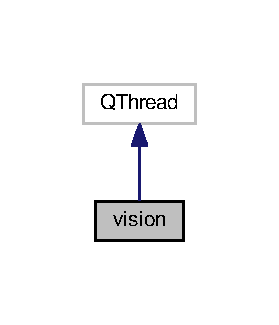
\includegraphics[width=134pt]{classvision__inherit__graph}
\end{center}
\end{figure}


Collaboration diagram for vision\+:
\nopagebreak
\begin{figure}[H]
\begin{center}
\leavevmode
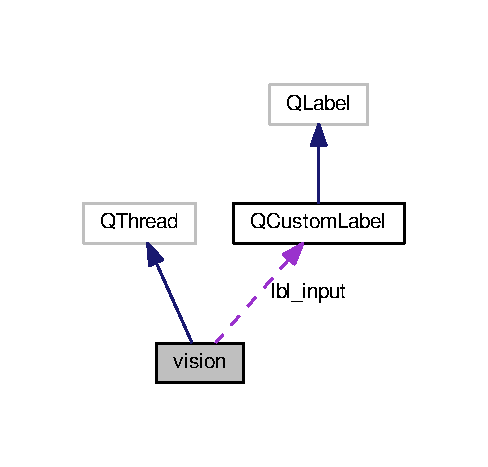
\includegraphics[width=234pt]{classvision__coll__graph}
\end{center}
\end{figure}
\subsection*{Public Member Functions}
\begin{DoxyCompactItemize}
\item 
void {\bfseries run} ()\hypertarget{classvision_ad213bf1ae76ed6a489390c501fe1b4e0}{}\label{classvision_ad213bf1ae76ed6a489390c501fe1b4e0}

\item 
void {\bfseries search\+\_\+color} (int)\hypertarget{classvision_a908d37e077c8844e2bfd5b38a1f65577}{}\label{classvision_a908d37e077c8844e2bfd5b38a1f65577}

\item 
void {\bfseries alloc\+\_\+calibration} (Calibration $\ast$)\hypertarget{classvision_a81fd57a35d8e331f844e1d276d8272f6}{}\label{classvision_a81fd57a35d8e331f844e1d276d8272f6}

\item 
void {\bfseries alloc\+\_\+state} (State $\ast$)\hypertarget{classvision_a4f8eec2ffc63e3a2b3e76c347b13f537}{}\label{classvision_a4f8eec2ffc63e3a2b3e76c347b13f537}

\item 
void {\bfseries alloc\+\_\+label\+\_\+input} (\hyperlink{classQCustomLabel}{Q\+Custom\+Label} $\ast$)\hypertarget{classvision_a5951eb6e1bb8582b3f01dec96d3ad3ac}{}\label{classvision_a5951eb6e1bb8582b3f01dec96d3ad3ac}

\item 
void {\bfseries alloc\+\_\+colors} (vector$<$ int $>$ $\ast$)\hypertarget{classvision_a5d366b880029815afed304c1d2d29bfc}{}\label{classvision_a5d366b880029815afed304c1d2d29bfc}

\item 
void {\bfseries alloc\+\_\+execution\+\_\+config} (Exec\+Configuration $\ast$)\hypertarget{classvision_a3d623a2e736f204716f1d44bf496823f}{}\label{classvision_a3d623a2e736f204716f1d44bf496823f}

\item 
void {\bfseries alloc\+\_\+label\+\_\+plots} (vector$<$ Q\+Label $\ast$ $>$ $\ast$)\hypertarget{classvision_a75142dd50f6818ae2d954a1070b7e721}{}\label{classvision_a75142dd50f6818ae2d954a1070b7e721}

\item 
void {\bfseries set\+\_\+device} (int)\hypertarget{classvision_af1d8cd9e34b8bd73d9c8b6eabc235936}{}\label{classvision_af1d8cd9e34b8bd73d9c8b6eabc235936}

\item 
void {\bfseries set\+\_\+id\+\_\+camera} (int)\hypertarget{classvision_adae525184ad84c63d1717f04c0df7453}{}\label{classvision_adae525184ad84c63d1717f04c0df7453}

\item 
void {\bfseries set\+\_\+path\+\_\+image} (string)\hypertarget{classvision_a28a5d8f9a27550c479cfd079d740bf8c}{}\label{classvision_a28a5d8f9a27550c479cfd079d740bf8c}

\item 
void {\bfseries set\+\_\+vision\+\_\+reception} (bool)\hypertarget{classvision_ad7906315a19d5828a862395b03405e66}{}\label{classvision_ad7906315a19d5828a862395b03405e66}

\item 
void {\bfseries set\+\_\+path\+\_\+video} (string)\hypertarget{classvision_ab200fa093a0d6520e17bbf9aa1e01819}{}\label{classvision_ab200fa093a0d6520e17bbf9aa1e01819}

\item 
int {\bfseries get\+\_\+device} ()\hypertarget{classvision_a73b97789728e71aef03d00c2b1ceff4f}{}\label{classvision_a73b97789728e71aef03d00c2b1ceff4f}

\item 
int {\bfseries get\+\_\+id\+\_\+camera} ()\hypertarget{classvision_a6b11affec899eac2e66fceba6ea12e62}{}\label{classvision_a6b11affec899eac2e66fceba6ea12e62}

\item 
string {\bfseries get\+\_\+path\+\_\+image} ()\hypertarget{classvision_a4127a06ad6e04c329100746954b8e41c}{}\label{classvision_a4127a06ad6e04c329100746954b8e41c}

\item 
bool {\bfseries get\+\_\+vision\+\_\+reception} ()\hypertarget{classvision_a830fb7eef3be9f1e6cdc341cfb2ba581}{}\label{classvision_a830fb7eef3be9f1e6cdc341cfb2ba581}

\item 
string {\bfseries get\+\_\+path\+\_\+video} ()\hypertarget{classvision_a6682f4c486ebbee30a65df223144d4ce}{}\label{classvision_a6682f4c486ebbee30a65df223144d4ce}

\item 
void {\bfseries finish} ()\hypertarget{classvision_a20d9a2c1134f59a53be852bdbf489c7b}{}\label{classvision_a20d9a2c1134f59a53be852bdbf489c7b}

\end{DoxyCompactItemize}
\subsection*{Protected Member Functions}
\begin{DoxyCompactItemize}
\item 
vector$<$ Rect $>$ {\bfseries order\+By\+Area} (vector$<$ Rect $>$)\hypertarget{classvision_af64ac1451112ad24c36ec25db081729e}{}\label{classvision_af64ac1451112ad24c36ec25db081729e}

\item 
Rect {\bfseries expand\+Rect} (Point)\hypertarget{classvision_a547beeec2c8fdf11eb3821071102e533}{}\label{classvision_a547beeec2c8fdf11eb3821071102e533}

\item 
bool {\bfseries its\+A\+Label} (Rect)\hypertarget{classvision_ae279754cc1e9370c3110f3ede4acae40}{}\label{classvision_ae279754cc1e9370c3110f3ede4acae40}

\item 
bool {\bfseries its\+Away\+From\+Limits} (Point)\hypertarget{classvision_acbbb21511dfafeb93ed58451c843d6f1}{}\label{classvision_acbbb21511dfafeb93ed58451c843d6f1}

\item 
void {\bfseries recognize\+Objects} ()\hypertarget{classvision_aa220323a006372ceebccab4a51498319}{}\label{classvision_aa220323a006372ceebccab4a51498319}

\item 
bool {\bfseries is\+Valid\+Point} (Point)\hypertarget{classvision_a63699f62d8601812f48a8b06ad8309f1}{}\label{classvision_a63699f62d8601812f48a8b06ad8309f1}

\item 
void {\bfseries update\+Plot} ()\hypertarget{classvision_a71ea3478a09dc629bcf7b4d84a27c4b7}{}\label{classvision_a71ea3478a09dc629bcf7b4d84a27c4b7}

\end{DoxyCompactItemize}
\subsection*{Protected Attributes}
\begin{DoxyCompactItemize}
\item 
bool {\bfseries run\+\_\+it}\hypertarget{classvision_aecb99ce2062a83e281a516779bc38e66}{}\label{classvision_aecb99ce2062a83e281a516779bc38e66}

\item 
bool {\bfseries start\+\_\+finish}\hypertarget{classvision_a4bf6d1ad7886c368201f01d68cd87960}{}\label{classvision_a4bf6d1ad7886c368201f01d68cd87960}

\item 
int {\bfseries device\+\_\+used}\hypertarget{classvision_a4489e26964fedb334f8a11323974d1a5}{}\label{classvision_a4489e26964fedb334f8a11323974d1a5}

\item 
int {\bfseries id\+\_\+camera}\hypertarget{classvision_aed0670889f7380c81cb3c6a9b0783399}{}\label{classvision_aed0670889f7380c81cb3c6a9b0783399}

\item 
bool {\bfseries vision\+\_\+reception}\hypertarget{classvision_a33c98ec05332bc5c29cb59b7aec7cbe9}{}\label{classvision_a33c98ec05332bc5c29cb59b7aec7cbe9}

\item 
string {\bfseries path\+\_\+image}\hypertarget{classvision_a1c8c4864b8690f6146e2d383a0e26f8a}{}\label{classvision_a1c8c4864b8690f6146e2d383a0e26f8a}

\item 
string {\bfseries path\+\_\+video}\hypertarget{classvision_a277365a0346f8f7e8abfcd5dea190706}{}\label{classvision_a277365a0346f8f7e8abfcd5dea190706}

\item 
int {\bfseries side\+\_\+cut}\hypertarget{classvision_ae465726320ce212e6d9ba02c98183a4c}{}\label{classvision_ae465726320ce212e6d9ba02c98183a4c}

\item 
float {\bfseries area\+\_\+min}\hypertarget{classvision_a394274c0683ad061464939b117ef8a34}{}\label{classvision_a394274c0683ad061464939b117ef8a34}

\item 
float {\bfseries area\+\_\+max}\hypertarget{classvision_acd9de3a225e3a560cb0d25546a3dec80}{}\label{classvision_acd9de3a225e3a560cb0d25546a3dec80}

\item 
float {\bfseries distc\+\_\+min}\hypertarget{classvision_a55d7e213d59603d7ac47a52b84109809}{}\label{classvision_a55d7e213d59603d7ac47a52b84109809}

\item 
float {\bfseries distc\+\_\+max}\hypertarget{classvision_a20c85db3ec02873d653e5bb9b10c39ff}{}\label{classvision_a20c85db3ec02873d653e5bb9b10c39ff}

\item 
float {\bfseries propc\+\_\+min}\hypertarget{classvision_a91f86b737be2111668b21ee63797f401}{}\label{classvision_a91f86b737be2111668b21ee63797f401}

\item 
float {\bfseries propc\+\_\+max}\hypertarget{classvision_a6aeb3bfbd1eebe0a8e1d722eb8c21891}{}\label{classvision_a6aeb3bfbd1eebe0a8e1d722eb8c21891}

\item 
Calibration $\ast$ {\bfseries calib}\hypertarget{classvision_a7e5420798a60cb8b48e8a29b786f1683}{}\label{classvision_a7e5420798a60cb8b48e8a29b786f1683}

\item 
State $\ast$ {\bfseries state}\hypertarget{classvision_a66846efba8a3de237d1a3c153ff1b812}{}\label{classvision_a66846efba8a3de237d1a3c153ff1b812}

\item 
Exec\+Configuration $\ast$ {\bfseries exec\+\_\+config}\hypertarget{classvision_a7929fc67b174048c25f34c064e6931ea}{}\label{classvision_a7929fc67b174048c25f34c064e6931ea}

\item 
Table\+Color {\bfseries table\+\_\+color}\hypertarget{classvision_a992a907eaa83feaa4fdec5eec0a3c978}{}\label{classvision_a992a907eaa83feaa4fdec5eec0a3c978}

\item 
Mat {\bfseries in}\hypertarget{classvision_a628e5f4db4cf2b380fa9849b1c7c6ede}{}\label{classvision_a628e5f4db4cf2b380fa9849b1c7c6ede}

\item 
Mat {\bfseries out}\hypertarget{classvision_a8e6f2872c854246898bdaf75db8bc219}{}\label{classvision_a8e6f2872c854246898bdaf75db8bc219}

\item 
Mat {\bfseries saved}\hypertarget{classvision_aaa8cc8d3f4860c2fe40b54d30ba3bb73}{}\label{classvision_aaa8cc8d3f4860c2fe40b54d30ba3bb73}

\item 
Mat {\bfseries raw\+\_\+out}\hypertarget{classvision_ae5f3eff88240c3cb76eb6b6018cc7fea}{}\label{classvision_ae5f3eff88240c3cb76eb6b6018cc7fea}

\item 
Mat {\bfseries raw\+\_\+in}\hypertarget{classvision_a8be17d4889ad9b9154f3d90825893b70}{}\label{classvision_a8be17d4889ad9b9154f3d90825893b70}

\item 
Mat {\bfseries storage}\hypertarget{classvision_adf6eda2658af488a78cbf3d4e9fc9612}{}\label{classvision_adf6eda2658af488a78cbf3d4e9fc9612}

\item 
Video\+Capture {\bfseries cap}\hypertarget{classvision_a6ce35c3216f36f741a0fab54e815d820}{}\label{classvision_a6ce35c3216f36f741a0fab54e815d820}

\item 
vector$<$ vector$<$ Point $>$ $>$ {\bfseries coordinate\+\_\+old}\hypertarget{classvision_a3d8aa1ce75f36f4bb0c2270100a1a0df}{}\label{classvision_a3d8aa1ce75f36f4bb0c2270100a1a0df}

\item 
vector$<$ vector$<$ Point $>$ $>$ {\bfseries labels}\hypertarget{classvision_a2a7fa3ec56b81484eb06c0f5c068365a}{}\label{classvision_a2a7fa3ec56b81484eb06c0f5c068365a}

\item 
vector$<$ vector$<$ Point $>$ $>$ {\bfseries contours}\hypertarget{classvision_a77ade58544c4db2587686e73d227cc37}{}\label{classvision_a77ade58544c4db2587686e73d227cc37}

\item 
vector$<$ Vec4i $>$ {\bfseries hierarchy}\hypertarget{classvision_a04a535405c5d7b076299073194f497b4}{}\label{classvision_a04a535405c5d7b076299073194f497b4}

\item 
vector$<$ Point $>$ {\bfseries vol\+\_\+coordinate}\hypertarget{classvision_a4f28ab3ac6e168aa977725da1973399b}{}\label{classvision_a4f28ab3ac6e168aa977725da1973399b}

\item 
vector$<$ int $>$ $\ast$ {\bfseries colors}\hypertarget{classvision_a7a1ac84ff70026be06b4ffe17fb0f3aa}{}\label{classvision_a7a1ac84ff70026be06b4ffe17fb0f3aa}

\item 
bool {\bfseries find\+\_\+old\+\_\+labels} \mbox{[}13\mbox{]}\hypertarget{classvision_a08b91dbb2384d4c6bd78560ec6621246}{}\label{classvision_a08b91dbb2384d4c6bd78560ec6621246}

\item 
Kalman\+Filter {\bfseries kfs} \mbox{[}13\mbox{]}\hypertarget{classvision_a76bf5d0bd645d4db2d9535bacae1284f}{}\label{classvision_a76bf5d0bd645d4db2d9535bacae1284f}

\item 
\hyperlink{classQCustomLabel}{Q\+Custom\+Label} $\ast$ {\bfseries lbl\+\_\+input}\hypertarget{classvision_ae925689fd0bd2eb2fcf2159e2f7b251e}{}\label{classvision_ae925689fd0bd2eb2fcf2159e2f7b251e}

\item 
vector$<$ Q\+Label $\ast$ $>$ $\ast$ {\bfseries lbl\+\_\+plots}\hypertarget{classvision_a4ec174995015376fcc9c15add83ed422}{}\label{classvision_a4ec174995015376fcc9c15add83ed422}

\end{DoxyCompactItemize}


The documentation for this class was generated from the following files\+:\begin{DoxyCompactItemize}
\item 
/home/johnathan/\+Repositories/\+S\+I\+R\+Lab/\+V\+S\+S-\/\+Vision/src/vision.\+h\item 
/home/johnathan/\+Repositories/\+S\+I\+R\+Lab/\+V\+S\+S-\/\+Vision/src/vision.\+cpp\end{DoxyCompactItemize}

\hypertarget{structcommon_1_1VisionColor}{}\section{common\+:\+:Vision\+Color Struct Reference}
\label{structcommon_1_1VisionColor}\index{common\+::\+Vision\+Color@{common\+::\+Vision\+Color}}


This struct represents a Color that can be calibrated\+: made by 2 Pixels that represents a range of color, Bottom \hyperlink{structcommon_1_1Pixel}{Pixel} Limit and Top \hyperlink{structcommon_1_1Pixel}{Pixel} Limit.  




{\ttfamily \#include $<$common.\+h$>$}



Collaboration diagram for common\+:\+:Vision\+Color\+:\nopagebreak
\begin{figure}[H]
\begin{center}
\leavevmode
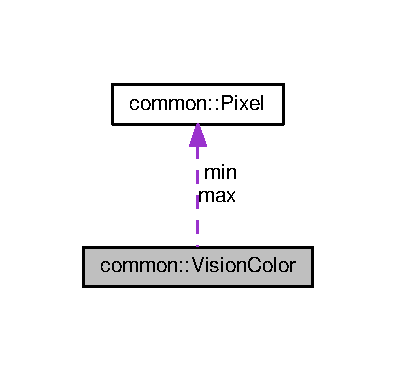
\includegraphics[width=190pt]{structcommon_1_1VisionColor__coll__graph}
\end{center}
\end{figure}
\subsection*{Public Member Functions}
\begin{DoxyCompactItemize}
\item 
\hyperlink{structcommon_1_1VisionColor_a5c458feb1d92c624dff7e83a4bfa50e5}{Vision\+Color} ()\hypertarget{structcommon_1_1VisionColor_a5c458feb1d92c624dff7e83a4bfa50e5}{}\label{structcommon_1_1VisionColor_a5c458feb1d92c624dff7e83a4bfa50e5}

\begin{DoxyCompactList}\small\item\em Constructor default\+: \hyperlink{structcommon_1_1VisionColor}{Vision\+Color} c;. \end{DoxyCompactList}\item 
\hyperlink{structcommon_1_1VisionColor_a3552e22bbdf84cecdcfbe39d729be767}{Vision\+Color} (\hyperlink{structcommon_1_1Pixel}{Pixel} \hyperlink{structcommon_1_1VisionColor_a3a8a40c24233df23f44510fce5846aaf}{min}, \hyperlink{structcommon_1_1Pixel}{Pixel} \hyperlink{structcommon_1_1VisionColor_adc2c9c3c09c9694f7ce8e9c8d94407bd}{max})\hypertarget{structcommon_1_1VisionColor_a3552e22bbdf84cecdcfbe39d729be767}{}\label{structcommon_1_1VisionColor_a3552e22bbdf84cecdcfbe39d729be767}

\begin{DoxyCompactList}\small\item\em Constructor Pixels\+: \hyperlink{structcommon_1_1VisionColor}{Vision\+Color} c( \hyperlink{structcommon_1_1Pixel}{Pixel} (r, g, b), \hyperlink{structcommon_1_1Pixel}{Pixel} (r, g, b));. \end{DoxyCompactList}\item 
\hyperlink{structcommon_1_1VisionColor_a547481e4da9d02d44c2687c36a7de4b9}{Vision\+Color} (\hyperlink{structcommon_1_1VisionColor}{Vision\+Color} $\ast$color)\hypertarget{structcommon_1_1VisionColor_a547481e4da9d02d44c2687c36a7de4b9}{}\label{structcommon_1_1VisionColor_a547481e4da9d02d44c2687c36a7de4b9}

\begin{DoxyCompactList}\small\item\em Constructor copy\+: \hyperlink{structcommon_1_1VisionColor}{Vision\+Color} c( Vision\+Color );. \end{DoxyCompactList}\item 
void \hyperlink{structcommon_1_1VisionColor_ab566eab8f4f6dda505e423bdaffc7d27}{show} ()\hypertarget{structcommon_1_1VisionColor_ab566eab8f4f6dda505e423bdaffc7d27}{}\label{structcommon_1_1VisionColor_ab566eab8f4f6dda505e423bdaffc7d27}

\begin{DoxyCompactList}\small\item\em Default function\+: prints all variables. \end{DoxyCompactList}\end{DoxyCompactItemize}
\subsection*{Public Attributes}
\begin{DoxyCompactItemize}
\item 
\hyperlink{structcommon_1_1Pixel}{Pixel} \hyperlink{structcommon_1_1VisionColor_a3a8a40c24233df23f44510fce5846aaf}{min}\hypertarget{structcommon_1_1VisionColor_a3a8a40c24233df23f44510fce5846aaf}{}\label{structcommon_1_1VisionColor_a3a8a40c24233df23f44510fce5846aaf}

\begin{DoxyCompactList}\small\item\em Data\+: Bottom \hyperlink{structcommon_1_1Pixel}{Pixel} Limit. \end{DoxyCompactList}\item 
\hyperlink{structcommon_1_1Pixel}{Pixel} \hyperlink{structcommon_1_1VisionColor_adc2c9c3c09c9694f7ce8e9c8d94407bd}{max}\hypertarget{structcommon_1_1VisionColor_adc2c9c3c09c9694f7ce8e9c8d94407bd}{}\label{structcommon_1_1VisionColor_adc2c9c3c09c9694f7ce8e9c8d94407bd}

\begin{DoxyCompactList}\small\item\em Data\+: Top \hyperlink{structcommon_1_1Pixel}{Pixel} Limit. \end{DoxyCompactList}\end{DoxyCompactItemize}


\subsection{Detailed Description}
This struct represents a Color that can be calibrated\+: made by 2 Pixels that represents a range of color, Bottom \hyperlink{structcommon_1_1Pixel}{Pixel} Limit and Top \hyperlink{structcommon_1_1Pixel}{Pixel} Limit. 

The documentation for this struct was generated from the following file\+:\begin{DoxyCompactItemize}
\item 
/home/johnathan/\+Repositories/\+S\+I\+R\+Lab/\+V\+S\+S-\/\+Vision/master/src/common.\+h\end{DoxyCompactItemize}

%--- End generated contents ---

% Index
\newpage
\phantomsection
\addcontentsline{toc}{chapter}{Index}
\printindex

\end{document}
